\documentclass[twoside]{book}

% Packages required by doxygen
\usepackage{calc}
\usepackage{doxygen}
\usepackage{graphicx}
\usepackage[utf8]{inputenc}
\usepackage{makeidx}
\usepackage{multicol}
\usepackage{multirow}
\usepackage{textcomp}
\usepackage[table]{xcolor}

% NLS support packages
\usepackage[catalan]{babel}

% Font selection
\usepackage[T1]{fontenc}
\usepackage{mathptmx}
\usepackage[scaled=.90]{helvet}
\usepackage{courier}
\usepackage{amssymb}
\usepackage{sectsty}
\renewcommand{\familydefault}{\sfdefault}
\allsectionsfont{%
  \fontseries{bc}\selectfont%
  \color{darkgray}%
}
\renewcommand{\DoxyLabelFont}{%
  \fontseries{bc}\selectfont%
  \color{darkgray}%
}

% Page & text layout
\usepackage{geometry}
\geometry{%
  a4paper,%
  top=2.5cm,%
  bottom=2.5cm,%
  left=2.5cm,%
  right=2.5cm%
}
\tolerance=750
\hfuzz=15pt
\hbadness=750
\setlength{\emergencystretch}{15pt}
\setlength{\parindent}{0cm}
\setlength{\parskip}{0.2cm}
\makeatletter
\renewcommand{\paragraph}{%
  \@startsection{paragraph}{4}{0ex}{-1.0ex}{1.0ex}{%
    \normalfont\normalsize\bfseries\SS@parafont%
  }%
}
\renewcommand{\subparagraph}{%
  \@startsection{subparagraph}{5}{0ex}{-1.0ex}{1.0ex}{%
    \normalfont\normalsize\bfseries\SS@subparafont%
  }%
}
\makeatother

% Headers & footers
\usepackage{fancyhdr}
\pagestyle{fancyplain}
\fancyhead[LE]{\fancyplain{}{\bfseries\thepage}}
\fancyhead[CE]{\fancyplain{}{}}
\fancyhead[RE]{\fancyplain{}{\bfseries\leftmark}}
\fancyhead[LO]{\fancyplain{}{\bfseries\rightmark}}
\fancyhead[CO]{\fancyplain{}{}}
\fancyhead[RO]{\fancyplain{}{\bfseries\thepage}}
\fancyfoot[LE]{\fancyplain{}{}}
\fancyfoot[CE]{\fancyplain{}{}}
\fancyfoot[RE]{\fancyplain{}{\bfseries\scriptsize Generat a Dc Dec 9 2015 20\-:45\-:00 per a Pràctica de P\-R\-O2. Supermercat. per Doxygen }}
\fancyfoot[LO]{\fancyplain{}{\bfseries\scriptsize Generat a Dc Dec 9 2015 20\-:45\-:00 per a Pràctica de P\-R\-O2. Supermercat. per Doxygen }}
\fancyfoot[CO]{\fancyplain{}{}}
\fancyfoot[RO]{\fancyplain{}{}}
\renewcommand{\footrulewidth}{0.4pt}
\renewcommand{\chaptermark}[1]{%
  \markboth{#1}{}%
}
\renewcommand{\sectionmark}[1]{%
  \markright{\thesection\ #1}%
}

% Indices & bibliography
\usepackage{natbib}
\usepackage[titles]{tocloft}
\setcounter{tocdepth}{3}
\setcounter{secnumdepth}{5}
\makeindex

% Hyperlinks (required, but should be loaded last)
\usepackage{ifpdf}
\ifpdf
  \usepackage[pdftex,pagebackref=true]{hyperref}
\else
  \usepackage[ps2pdf,pagebackref=true]{hyperref}
\fi
\hypersetup{%
  colorlinks=true,%
  linkcolor=blue,%
  citecolor=blue,%
  unicode%
}

% Custom commands
\newcommand{\clearemptydoublepage}{%
  \newpage{\pagestyle{empty}\cleardoublepage}%
}


%===== C O N T E N T S =====

\begin{document}

% Titlepage & ToC
\hypersetup{pageanchor=false}
\pagenumbering{roman}
\begin{titlepage}
\vspace*{7cm}
\begin{center}%
{\Large Pràctica de P\-R\-O2. Supermercat. \\[1ex]\large versió dec-\/2015 }\\
\vspace*{1cm}
{\large Generat per Doxygen 1.8.6}\\
\vspace*{0.5cm}
{\small Dc Dec 9 2015 20:45:00}\\
\end{center}
\end{titlepage}
\clearemptydoublepage
\tableofcontents
\clearemptydoublepage
\pagenumbering{arabic}
\hypersetup{pageanchor=true}

%--- Begin generated contents ---
\chapter{Índex de Classes}
\section{Llista de Classes}
Aquestes són les classes, estructures, unions i interfícies acompanyades amb breus descripcions\-:\begin{DoxyCompactList}
\item\contentsline{section}{\hyperlink{struct_caixa}{Caixa} }{\pageref{struct_caixa}}{}
\item\contentsline{section}{\hyperlink{class_client}{Client} \\*Respresenta un \hyperlink{class_client}{Client} com a contenidor de Seccions i \hyperlink{class_temps}{Temps} }{\pageref{class_client}}{}
\item\contentsline{section}{\hyperlink{class_conjunt__clients}{Conjunt\-\_\-clients} \\*Respresenta un Conjunt de clients com a contenidor de Clients }{\pageref{class_conjunt__clients}}{}
\item\contentsline{section}{\hyperlink{class_conjunt__productes}{Conjunt\-\_\-productes} \\*Respresenta un Conjunt de productes con a contenidor de Productes }{\pageref{class_conjunt__productes}}{}
\item\contentsline{section}{\hyperlink{class_producte}{Producte} \\*Respresenta un \hyperlink{class_producte}{Producte} com a contenidor d'un id, la seva posició a la graella, un temps de cobrament i un preu }{\pageref{class_producte}}{}
\item\contentsline{section}{\hyperlink{structseccio}{seccio} }{\pageref{structseccio}}{}
\item\contentsline{section}{\hyperlink{class_supermercat}{Supermercat} \\*Respresenta un \hyperlink{class_supermercat}{Supermercat} com a contenidor de Matriu de sets i un vector de Caixes }{\pageref{class_supermercat}}{}
\item\contentsline{section}{\hyperlink{class_temps}{Temps} \\*Respresentacio del temps en hores,minuts i segons }{\pageref{class_temps}}{}
\end{DoxyCompactList}

\chapter{Índex de Fitxers}
\section{Llista dels Fitxers}
Aquesta és la llista de tots els fitxers acompanyats amb breus descripcions\-:\begin{DoxyCompactList}
\item\contentsline{section}{\hyperlink{_client_8cc}{Client.\-cc} }{\pageref{_client_8cc}}{}
\item\contentsline{section}{\hyperlink{_client_8hh}{Client.\-hh} \\*Classe \hyperlink{class_client}{Client} }{\pageref{_client_8hh}}{}
\item\contentsline{section}{\hyperlink{_conjunt__clients_8cc}{Conjunt\-\_\-clients.\-cc} }{\pageref{_conjunt__clients_8cc}}{}
\item\contentsline{section}{\hyperlink{_conjunt__clients_8hh}{Conjunt\-\_\-clients.\-hh} \\*Classe \hyperlink{class_conjunt__clients}{Conjunt\-\_\-clients} }{\pageref{_conjunt__clients_8hh}}{}
\item\contentsline{section}{\hyperlink{_conjunt__productes_8cc}{Conjunt\-\_\-productes.\-cc} }{\pageref{_conjunt__productes_8cc}}{}
\item\contentsline{section}{\hyperlink{_conjunt__productes_8hh}{Conjunt\-\_\-productes.\-hh} \\*Classe \hyperlink{class_conjunt__productes}{Conjunt\-\_\-productes} }{\pageref{_conjunt__productes_8hh}}{}
\item\contentsline{section}{\hyperlink{_producte_8cc}{Producte.\-cc} }{\pageref{_producte_8cc}}{}
\item\contentsline{section}{\hyperlink{_producte_8hh}{Producte.\-hh} \\*Classe \hyperlink{class_producte}{Producte} }{\pageref{_producte_8hh}}{}
\item\contentsline{section}{\hyperlink{program_8cc}{program.\-cc} }{\pageref{program_8cc}}{}
\item\contentsline{section}{\hyperlink{_supermercat_8cc}{Supermercat.\-cc} }{\pageref{_supermercat_8cc}}{}
\item\contentsline{section}{\hyperlink{_supermercat_8hh}{Supermercat.\-hh} \\*Classe \hyperlink{class_supermercat}{Supermercat} }{\pageref{_supermercat_8hh}}{}
\item\contentsline{section}{\hyperlink{_temps_8cc}{Temps.\-cc} }{\pageref{_temps_8cc}}{}
\item\contentsline{section}{\hyperlink{_temps_8hh}{Temps.\-hh} \\*Classe \hyperlink{class_temps}{Temps} }{\pageref{_temps_8hh}}{}
\end{DoxyCompactList}

\chapter{Documentació de les Classes}
\hypertarget{struct_caixa}{\section{Referència de l'Estructura Caixa}
\label{struct_caixa}\index{Caixa@{Caixa}}
}
\subsection*{Atributs Públics}
\begin{DoxyCompactItemize}
\item 
int \hyperlink{struct_caixa_af62e7e1b599b3e57cb0f2f961335f914}{n\-\_\-clients}
\item 
\hyperlink{class_temps}{Temps} \hyperlink{struct_caixa_a1bdc14d5913064368efb726816d76d0c}{instant\-\_\-proxim}
\end{DoxyCompactItemize}


\subsection{Descripció Detallada}


Definició a la línia 18 del fitxer Supermercat.\-hh.



\subsection{Documentació de les Dades Membre}
\hypertarget{struct_caixa_af62e7e1b599b3e57cb0f2f961335f914}{\index{Caixa@{Caixa}!n\-\_\-clients@{n\-\_\-clients}}
\index{n\-\_\-clients@{n\-\_\-clients}!Caixa@{Caixa}}
\subsubsection[{n\-\_\-clients}]{\setlength{\rightskip}{0pt plus 5cm}int Caixa\-::n\-\_\-clients}}\label{struct_caixa_af62e7e1b599b3e57cb0f2f961335f914}


Definició a la línia 19 del fitxer Supermercat.\-hh.

\hypertarget{struct_caixa_a1bdc14d5913064368efb726816d76d0c}{\index{Caixa@{Caixa}!instant\-\_\-proxim@{instant\-\_\-proxim}}
\index{instant\-\_\-proxim@{instant\-\_\-proxim}!Caixa@{Caixa}}
\subsubsection[{instant\-\_\-proxim}]{\setlength{\rightskip}{0pt plus 5cm}{\bf Temps} Caixa\-::instant\-\_\-proxim}}\label{struct_caixa_a1bdc14d5913064368efb726816d76d0c}


Definició a la línia 20 del fitxer Supermercat.\-hh.



La documentació d'aquesta estructura es va generar a partir del següent fitxer\-:\begin{DoxyCompactItemize}
\item 
\hyperlink{_supermercat_8hh}{Supermercat.\-hh}\end{DoxyCompactItemize}

\hypertarget{class_client}{\section{Referència de la Classe Client}
\label{class_client}\index{Client@{Client}}
}


Respresenta un \hyperlink{class_client}{Client} com a contenidor de Seccions i \hyperlink{class_temps}{Temps}.  


\subsection*{Mètodes públics}
\begin{DoxyCompactItemize}
\item 
\hyperlink{class_client_ae51af7aa6b8f591496a8f6a4a87a14bf}{Client} ()
\item 
\hyperlink{class_client_a493e90fe1fed012b37d2831734fed67a}{Client} (int identificador\-\_\-p, \hyperlink{class_temps}{Temps} t\-\_\-p, int nombre\-\_\-productes\-\_\-p)
\begin{DoxyCompactList}\small\item\em Constructora per defecte. \end{DoxyCompactList}\item 
\hyperlink{class_client_a840e519ca781888cbd54181572ebe3a7}{$\sim$\-Client} ()
\begin{DoxyCompactList}\small\item\em Crea un client amb els parametres rebuts. \end{DoxyCompactList}\item 
int \hyperlink{class_client_ab9db667f1961595d18c33d81f082aba0}{consultar\-\_\-identificador} ()
\begin{DoxyCompactList}\small\item\em Destructora per defecte. \end{DoxyCompactList}\item 
int \hyperlink{class_client_ab6d7b4f334942edf741a06933f93d9ab}{consultar\-\_\-caixa} ()
\begin{DoxyCompactList}\small\item\em Retorna l'identificador d'un client. \end{DoxyCompactList}\item 
\hyperlink{class_temps}{Temps} \hyperlink{class_client_ae56fc1628dfb8b857a2cc0663b4989e8}{consultar\-\_\-instant\-\_\-tiquet} ()
\begin{DoxyCompactList}\small\item\em Retorna la caixa assignada d'un client. \end{DoxyCompactList}\item 
\hyperlink{class_temps}{Temps} \hyperlink{class_client_a5b08c2bce4406280925869212a0831d9}{consultar\-\_\-instant\-\_\-caixa} ()
\begin{DoxyCompactList}\small\item\em Retorna el moment de recollida del tiquet. \end{DoxyCompactList}\item 
int \hyperlink{class_client_af3c1754dbbd0593c30cb6ffa8ddef086}{consultar\-\_\-productes\-\_\-client} ()
\begin{DoxyCompactList}\small\item\em Consulta l'instant de caixa del p.\-implicit. \end{DoxyCompactList}\item 
\hyperlink{class_temps}{Temps} \hyperlink{class_client_a2ccbf48235fab996aff2bb9d31e03b67}{consultar\-\_\-temps\-\_\-cobrament} ()
\begin{DoxyCompactList}\small\item\em Retorna el nombre de productes d'un \hyperlink{class_client}{Client}. \end{DoxyCompactList}\item 
\hyperlink{class_temps}{Temps} \hyperlink{class_client_a94e4cd3e3d2c3e675d9e722a7e402963}{consultar\-\_\-temps\-\_\-espera\-\_\-cua} ()
\begin{DoxyCompactList}\small\item\em Consulta el temps total que trigara el p. implicit en pagar. \end{DoxyCompactList}\item 
\hyperlink{class_temps}{Temps} \hyperlink{class_client_a0a7ef70f7ad923d76f0982aa616ebf0c}{consultar\-\_\-instant\-\_\-cua} ()
\begin{DoxyCompactList}\small\item\em Consulta el temps d'espera que trigara el p. implicit a la cua. \end{DoxyCompactList}\item 
\hyperlink{class_temps}{Temps} \hyperlink{class_client_a0f893a0ad60702dacd2c2502d6b2aec3}{consultar\-\_\-instant\-\_\-acabament} ()
\begin{DoxyCompactList}\small\item\em Consulta l'instant en el que el p.\-implicit arriba a la cua. \end{DoxyCompactList}\item 
void \hyperlink{class_client_afb5ec40f5410ec9766ca3c225add1d93}{modificar\-\_\-instant\-\_\-cua} (\hyperlink{class_temps}{Temps} t)
\begin{DoxyCompactList}\small\item\em Consulta l'instant en el que el p.\-implicit acaba. \end{DoxyCompactList}\item 
void \hyperlink{class_client_abb16904da37ead035413d5595889af2f}{modificar\-\_\-instant\-\_\-acabament} (\hyperlink{class_temps}{Temps} instant\-\_\-acabament\-\_\-p)
\begin{DoxyCompactList}\small\item\em Modifica l'instant en el que el p.\-implicit arriba a la cua. \end{DoxyCompactList}\item 
void \hyperlink{class_client_aa3c794239505f1996f1468a542548461}{modificar\-\_\-caixa} (int caixa\-\_\-p)
\begin{DoxyCompactList}\small\item\em Modifica al P.\-I. l'instant d'acabament. \end{DoxyCompactList}\item 
void \hyperlink{class_client_a358215e753f86584d9159d01b66eeded}{modificar\-\_\-temps\-\_\-cobrament} (\hyperlink{class_temps}{Temps} n)
\begin{DoxyCompactList}\small\item\em Modifica la caixa assignada del p.\-implicit. \end{DoxyCompactList}\item 
void \hyperlink{class_client_a8ea63f73665f9384629d2a6ff46bb252}{modificar\-\_\-temps\-\_\-espera\-\_\-cua} (\hyperlink{class_temps}{Temps} n)
\begin{DoxyCompactList}\small\item\em Modifica el temps de cobrament del p.\-implicit. \end{DoxyCompactList}\item 
void \hyperlink{class_client_ab9604d012fe1763e9b26c0579354d7c8}{modificar\-\_\-temps\-\_\-caminar} (int t)
\begin{DoxyCompactList}\small\item\em Modifica el temps d'espera a la cua del p.\-implicit. \end{DoxyCompactList}\item 
void \hyperlink{class_client_a1718ce0ec5713509921963aaa48f6417}{modificar\-\_\-instant\-\_\-caixa} (\hyperlink{class_temps}{Temps} t)
\begin{DoxyCompactList}\small\item\em Modifica el temps de caminar del p.\-implicit. \end{DoxyCompactList}\item 
void \hyperlink{class_client_a7aa5563129732582a21cefb39fa88e9e}{llegeix\-\_\-client} (\hyperlink{class_conjunt__productes}{Conjunt\-\_\-productes} \&cp)
\begin{DoxyCompactList}\small\item\em Modifica l'instant de caixa del p.\-implicit. \end{DoxyCompactList}\item 
void \hyperlink{class_client_a04bd02ce8b35ecae1656367ccadf6354}{llegir\-\_\-conjunt\-\_\-productes} (int n, \hyperlink{class_conjunt__productes}{Conjunt\-\_\-productes} \&c)
\begin{DoxyCompactList}\small\item\em Llegeix un client pel canal estandard. \end{DoxyCompactList}\item 
void \hyperlink{class_client_a727c33533aae0c3e3e77eac10cf9e3c6}{consulta\-\_\-millor\-\_\-cami} (int rengles)
\begin{DoxyCompactList}\small\item\em Llegeix un conjunt de productes i s'afegeix al \hyperlink{class_client}{Client}. \end{DoxyCompactList}\end{DoxyCompactItemize}


\subsection{Descripció Detallada}
Respresenta un \hyperlink{class_client}{Client} com a contenidor de Seccions i \hyperlink{class_temps}{Temps}. 

Definició a la línia 29 del fitxer Client.\-hh.



\subsection{Documentació del Constructor i el Destructor}
\hypertarget{class_client_ae51af7aa6b8f591496a8f6a4a87a14bf}{\index{Client@{Client}!Client@{Client}}
\index{Client@{Client}!Client@{Client}}
\subsubsection[{Client}]{\setlength{\rightskip}{0pt plus 5cm}Client\-::\-Client (
\begin{DoxyParamCaption}
{}
\end{DoxyParamCaption}
)}}\label{class_client_ae51af7aa6b8f591496a8f6a4a87a14bf}


Definició a la línia 4 del fitxer Client.\-cc.


\begin{DoxyCode}
4               \{
5     
6     
7 \}
\end{DoxyCode}
\hypertarget{class_client_a493e90fe1fed012b37d2831734fed67a}{\index{Client@{Client}!Client@{Client}}
\index{Client@{Client}!Client@{Client}}
\subsubsection[{Client}]{\setlength{\rightskip}{0pt plus 5cm}Client\-::\-Client (
\begin{DoxyParamCaption}
\item[{int}]{identificador\-\_\-p, }
\item[{{\bf Temps}}]{t\-\_\-p, }
\item[{int}]{nombre\-\_\-productes\-\_\-p}
\end{DoxyParamCaption}
)}}\label{class_client_a493e90fe1fed012b37d2831734fed67a}


Constructora per defecte. 

\hypertarget{class_client_a840e519ca781888cbd54181572ebe3a7}{\index{Client@{Client}!$\sim$\-Client@{$\sim$\-Client}}
\index{$\sim$\-Client@{$\sim$\-Client}!Client@{Client}}
\subsubsection[{$\sim$\-Client}]{\setlength{\rightskip}{0pt plus 5cm}Client\-::$\sim$\-Client (
\begin{DoxyParamCaption}
{}
\end{DoxyParamCaption}
)}}\label{class_client_a840e519ca781888cbd54181572ebe3a7}


Crea un client amb els parametres rebuts. 

\begin{DoxyPrecond}{Precondició}
cert 
\end{DoxyPrecond}
\begin{DoxyPostcond}{Postcondició}
crea un \hyperlink{class_client}{Client} amb els parametres identificador, t... rebuts. 
\end{DoxyPostcond}


Definició a la línia 9 del fitxer Client.\-cc.


\begin{DoxyCode}
9 \{\}
\end{DoxyCode}


\subsection{Documentació de les Funcions Membre}
\hypertarget{class_client_ab9db667f1961595d18c33d81f082aba0}{\index{Client@{Client}!consultar\-\_\-identificador@{consultar\-\_\-identificador}}
\index{consultar\-\_\-identificador@{consultar\-\_\-identificador}!Client@{Client}}
\subsubsection[{consultar\-\_\-identificador}]{\setlength{\rightskip}{0pt plus 5cm}int Client\-::consultar\-\_\-identificador (
\begin{DoxyParamCaption}
{}
\end{DoxyParamCaption}
)}}\label{class_client_ab9db667f1961595d18c33d81f082aba0}


Destructora per defecte. 



Definició a la línia 19 del fitxer Client.\-cc.


\begin{DoxyCode}
19                                     \{
20     \textcolor{keywordflow}{return} identificador;
21 \}
\end{DoxyCode}
\hypertarget{class_client_ab6d7b4f334942edf741a06933f93d9ab}{\index{Client@{Client}!consultar\-\_\-caixa@{consultar\-\_\-caixa}}
\index{consultar\-\_\-caixa@{consultar\-\_\-caixa}!Client@{Client}}
\subsubsection[{consultar\-\_\-caixa}]{\setlength{\rightskip}{0pt plus 5cm}int Client\-::consultar\-\_\-caixa (
\begin{DoxyParamCaption}
{}
\end{DoxyParamCaption}
)}}\label{class_client_ab6d7b4f334942edf741a06933f93d9ab}


Retorna l'identificador d'un client. 

\begin{DoxyPrecond}{Precondició}
cert 
\end{DoxyPrecond}
\begin{DoxyPostcond}{Postcondició}
retorna l'identificador del client del p. implicit 
\end{DoxyPostcond}


Definició a la línia 15 del fitxer Client.\-cc.


\begin{DoxyCode}
15                            \{
16   \textcolor{keywordflow}{return} caixa;
17 \}
\end{DoxyCode}
\hypertarget{class_client_ae56fc1628dfb8b857a2cc0663b4989e8}{\index{Client@{Client}!consultar\-\_\-instant\-\_\-tiquet@{consultar\-\_\-instant\-\_\-tiquet}}
\index{consultar\-\_\-instant\-\_\-tiquet@{consultar\-\_\-instant\-\_\-tiquet}!Client@{Client}}
\subsubsection[{consultar\-\_\-instant\-\_\-tiquet}]{\setlength{\rightskip}{0pt plus 5cm}{\bf Temps} Client\-::consultar\-\_\-instant\-\_\-tiquet (
\begin{DoxyParamCaption}
{}
\end{DoxyParamCaption}
)}}\label{class_client_ae56fc1628dfb8b857a2cc0663b4989e8}


Retorna la caixa assignada d'un client. 

\begin{DoxyPrecond}{Precondició}
cert 
\end{DoxyPrecond}
\begin{DoxyPostcond}{Postcondició}
retorna la caixa assignada d'un client 
\end{DoxyPostcond}


Definició a la línia 44 del fitxer Client.\-cc.


\begin{DoxyCode}
44                                        \{
45     \textcolor{keywordflow}{return} instant\_tiquet;
46 \}
\end{DoxyCode}
\hypertarget{class_client_a5b08c2bce4406280925869212a0831d9}{\index{Client@{Client}!consultar\-\_\-instant\-\_\-caixa@{consultar\-\_\-instant\-\_\-caixa}}
\index{consultar\-\_\-instant\-\_\-caixa@{consultar\-\_\-instant\-\_\-caixa}!Client@{Client}}
\subsubsection[{consultar\-\_\-instant\-\_\-caixa}]{\setlength{\rightskip}{0pt plus 5cm}{\bf Temps} Client\-::consultar\-\_\-instant\-\_\-caixa (
\begin{DoxyParamCaption}
{}
\end{DoxyParamCaption}
)}}\label{class_client_a5b08c2bce4406280925869212a0831d9}


Retorna el moment de recollida del tiquet. 

\begin{DoxyPrecond}{Precondició}
El \hyperlink{class_client}{Client} ha recollit el tiquet 
\end{DoxyPrecond}
\begin{DoxyPostcond}{Postcondició}
retorna l'instant de recollida del parametre implicit 
\end{DoxyPostcond}


Definició a la línia 31 del fitxer Client.\-cc.


\begin{DoxyCode}
31                                       \{
32     \textcolor{keywordflow}{return} instant\_caixa;
33 \}
\end{DoxyCode}
\hypertarget{class_client_af3c1754dbbd0593c30cb6ffa8ddef086}{\index{Client@{Client}!consultar\-\_\-productes\-\_\-client@{consultar\-\_\-productes\-\_\-client}}
\index{consultar\-\_\-productes\-\_\-client@{consultar\-\_\-productes\-\_\-client}!Client@{Client}}
\subsubsection[{consultar\-\_\-productes\-\_\-client}]{\setlength{\rightskip}{0pt plus 5cm}int Client\-::consultar\-\_\-productes\-\_\-client (
\begin{DoxyParamCaption}
{}
\end{DoxyParamCaption}
)}}\label{class_client_af3c1754dbbd0593c30cb6ffa8ddef086}


Consulta l'instant de caixa del p.\-implicit. 

\begin{DoxyPrecond}{Precondició}
Cert 
\end{DoxyPrecond}
\begin{DoxyPostcond}{Postcondició}
Retorna l'instan de caixa del p.\-implicit 
\end{DoxyPostcond}


Definició a la línia 11 del fitxer Client.\-cc.


\begin{DoxyCode}
11                                        \{
12     \textcolor{keywordflow}{return} nombre\_productes;
13 \}
\end{DoxyCode}
\hypertarget{class_client_a2ccbf48235fab996aff2bb9d31e03b67}{\index{Client@{Client}!consultar\-\_\-temps\-\_\-cobrament@{consultar\-\_\-temps\-\_\-cobrament}}
\index{consultar\-\_\-temps\-\_\-cobrament@{consultar\-\_\-temps\-\_\-cobrament}!Client@{Client}}
\subsubsection[{consultar\-\_\-temps\-\_\-cobrament}]{\setlength{\rightskip}{0pt plus 5cm}{\bf Temps} Client\-::consultar\-\_\-temps\-\_\-cobrament (
\begin{DoxyParamCaption}
{}
\end{DoxyParamCaption}
)}}\label{class_client_a2ccbf48235fab996aff2bb9d31e03b67}


Retorna el nombre de productes d'un \hyperlink{class_client}{Client}. 

\begin{DoxyPrecond}{Precondició}
cert 
\end{DoxyPrecond}
\begin{DoxyPostcond}{Postcondició}
retorna el nombre de productes que te el p. implicit 
\end{DoxyPostcond}


Definició a la línia 23 del fitxer Client.\-cc.


\begin{DoxyCode}
23                                         \{
24     \textcolor{keywordflow}{return} temps\_cobrament;
25 \}
\end{DoxyCode}
\hypertarget{class_client_a94e4cd3e3d2c3e675d9e722a7e402963}{\index{Client@{Client}!consultar\-\_\-temps\-\_\-espera\-\_\-cua@{consultar\-\_\-temps\-\_\-espera\-\_\-cua}}
\index{consultar\-\_\-temps\-\_\-espera\-\_\-cua@{consultar\-\_\-temps\-\_\-espera\-\_\-cua}!Client@{Client}}
\subsubsection[{consultar\-\_\-temps\-\_\-espera\-\_\-cua}]{\setlength{\rightskip}{0pt plus 5cm}{\bf Temps} Client\-::consultar\-\_\-temps\-\_\-espera\-\_\-cua (
\begin{DoxyParamCaption}
{}
\end{DoxyParamCaption}
)}}\label{class_client_a94e4cd3e3d2c3e675d9e722a7e402963}


Consulta el temps total que trigara el p. implicit en pagar. 

\begin{DoxyPrecond}{Precondició}
Cert 
\end{DoxyPrecond}
\begin{DoxyPostcond}{Postcondició}
retorna el temps\-\_\-cobrament del p.\-implicit 
\end{DoxyPostcond}


Definició a la línia 113 del fitxer Client.\-cc.


\begin{DoxyCode}
113                                          \{
114     \textcolor{keywordflow}{return} temps\_espera\_cua;
115 \}
\end{DoxyCode}
\hypertarget{class_client_a0a7ef70f7ad923d76f0982aa616ebf0c}{\index{Client@{Client}!consultar\-\_\-instant\-\_\-cua@{consultar\-\_\-instant\-\_\-cua}}
\index{consultar\-\_\-instant\-\_\-cua@{consultar\-\_\-instant\-\_\-cua}!Client@{Client}}
\subsubsection[{consultar\-\_\-instant\-\_\-cua}]{\setlength{\rightskip}{0pt plus 5cm}{\bf Temps} Client\-::consultar\-\_\-instant\-\_\-cua (
\begin{DoxyParamCaption}
{}
\end{DoxyParamCaption}
)}}\label{class_client_a0a7ef70f7ad923d76f0982aa616ebf0c}


Consulta el temps d'espera que trigara el p. implicit a la cua. 

\begin{DoxyPrecond}{Precondició}
Cert 
\end{DoxyPrecond}
\begin{DoxyPostcond}{Postcondició}
retorna el temps\-\_\-espera del p.\-miplicit 
\end{DoxyPostcond}


Definició a la línia 121 del fitxer Client.\-cc.


\begin{DoxyCode}
121                                     \{
122     \textcolor{keywordflow}{return} instant\_cua;
123 \}
\end{DoxyCode}
\hypertarget{class_client_a0f893a0ad60702dacd2c2502d6b2aec3}{\index{Client@{Client}!consultar\-\_\-instant\-\_\-acabament@{consultar\-\_\-instant\-\_\-acabament}}
\index{consultar\-\_\-instant\-\_\-acabament@{consultar\-\_\-instant\-\_\-acabament}!Client@{Client}}
\subsubsection[{consultar\-\_\-instant\-\_\-acabament}]{\setlength{\rightskip}{0pt plus 5cm}{\bf Temps} Client\-::consultar\-\_\-instant\-\_\-acabament (
\begin{DoxyParamCaption}
{}
\end{DoxyParamCaption}
)}}\label{class_client_a0f893a0ad60702dacd2c2502d6b2aec3}


Consulta l'instant en el que el p.\-implicit arriba a la cua. 

\begin{DoxyPrecond}{Precondició}
Cert 
\end{DoxyPrecond}
\begin{DoxyPostcond}{Postcondició}
Retorna l'instant de cua del p.\-implicit 
\end{DoxyPostcond}


Definició a la línia 117 del fitxer Client.\-cc.


\begin{DoxyCode}
117                                           \{
118     \textcolor{keywordflow}{return} instant\_acabament;
119 \}
\end{DoxyCode}
\hypertarget{class_client_afb5ec40f5410ec9766ca3c225add1d93}{\index{Client@{Client}!modificar\-\_\-instant\-\_\-cua@{modificar\-\_\-instant\-\_\-cua}}
\index{modificar\-\_\-instant\-\_\-cua@{modificar\-\_\-instant\-\_\-cua}!Client@{Client}}
\subsubsection[{modificar\-\_\-instant\-\_\-cua}]{\setlength{\rightskip}{0pt plus 5cm}void Client\-::modificar\-\_\-instant\-\_\-cua (
\begin{DoxyParamCaption}
\item[{{\bf Temps}}]{t}
\end{DoxyParamCaption}
)}}\label{class_client_afb5ec40f5410ec9766ca3c225add1d93}


Consulta l'instant en el que el p.\-implicit acaba. 

\begin{DoxyPrecond}{Precondició}
Cert 
\end{DoxyPrecond}
\begin{DoxyPostcond}{Postcondició}
Retorna l'instant d'acabament del p.\-implicit 
\end{DoxyPostcond}


Definició a la línia 27 del fitxer Client.\-cc.


\begin{DoxyCode}
27                                          \{
28     instant\_cua = t;
29 \}
\end{DoxyCode}
\hypertarget{class_client_abb16904da37ead035413d5595889af2f}{\index{Client@{Client}!modificar\-\_\-instant\-\_\-acabament@{modificar\-\_\-instant\-\_\-acabament}}
\index{modificar\-\_\-instant\-\_\-acabament@{modificar\-\_\-instant\-\_\-acabament}!Client@{Client}}
\subsubsection[{modificar\-\_\-instant\-\_\-acabament}]{\setlength{\rightskip}{0pt plus 5cm}void Client\-::modificar\-\_\-instant\-\_\-acabament (
\begin{DoxyParamCaption}
\item[{{\bf Temps}}]{instant\-\_\-acabament\-\_\-p}
\end{DoxyParamCaption}
)}}\label{class_client_abb16904da37ead035413d5595889af2f}


Modifica l'instant en el que el p.\-implicit arriba a la cua. 

\begin{DoxyPrecond}{Precondició}
Cert 
\end{DoxyPrecond}
\begin{DoxyPostcond}{Postcondició}
El p.\-implicit passa a tenir com a instant\-\_\-cua t 
\end{DoxyPostcond}


Definició a la línia 39 del fitxer Client.\-cc.


\begin{DoxyCode}
39                                                 \{
40     instant\_acabament = t;
41 \}
\end{DoxyCode}
\hypertarget{class_client_aa3c794239505f1996f1468a542548461}{\index{Client@{Client}!modificar\-\_\-caixa@{modificar\-\_\-caixa}}
\index{modificar\-\_\-caixa@{modificar\-\_\-caixa}!Client@{Client}}
\subsubsection[{modificar\-\_\-caixa}]{\setlength{\rightskip}{0pt plus 5cm}void Client\-::modificar\-\_\-caixa (
\begin{DoxyParamCaption}
\item[{int}]{caixa\-\_\-p}
\end{DoxyParamCaption}
)}}\label{class_client_aa3c794239505f1996f1468a542548461}


Modifica al P.\-I. l'instant d'acabament. 

\begin{DoxyPrecond}{Precondició}
cert 
\end{DoxyPrecond}
\begin{DoxyPostcond}{Postcondició}
modifica al P.\-I. l'instant d'acabament 
\end{DoxyPostcond}


Definició a la línia 48 del fitxer Client.\-cc.


\begin{DoxyCode}
48                                        \{
49   caixa = caixa\_p;
50 \}
\end{DoxyCode}
\hypertarget{class_client_a358215e753f86584d9159d01b66eeded}{\index{Client@{Client}!modificar\-\_\-temps\-\_\-cobrament@{modificar\-\_\-temps\-\_\-cobrament}}
\index{modificar\-\_\-temps\-\_\-cobrament@{modificar\-\_\-temps\-\_\-cobrament}!Client@{Client}}
\subsubsection[{modificar\-\_\-temps\-\_\-cobrament}]{\setlength{\rightskip}{0pt plus 5cm}void Client\-::modificar\-\_\-temps\-\_\-cobrament (
\begin{DoxyParamCaption}
\item[{{\bf Temps}}]{n}
\end{DoxyParamCaption}
)}}\label{class_client_a358215e753f86584d9159d01b66eeded}


Modifica la caixa assignada del p.\-implicit. 

\begin{DoxyPrecond}{Precondició}
cert 
\end{DoxyPrecond}
\begin{DoxyPostcond}{Postcondició}
la caixa assignada del p.\-implicit passa a ser caixa\-\_\-p 
\end{DoxyPostcond}


Definició a la línia 101 del fitxer Client.\-cc.


\begin{DoxyCode}
101                                              \{
102     temps\_cobrament = n;
103 \}
\end{DoxyCode}
\hypertarget{class_client_a8ea63f73665f9384629d2a6ff46bb252}{\index{Client@{Client}!modificar\-\_\-temps\-\_\-espera\-\_\-cua@{modificar\-\_\-temps\-\_\-espera\-\_\-cua}}
\index{modificar\-\_\-temps\-\_\-espera\-\_\-cua@{modificar\-\_\-temps\-\_\-espera\-\_\-cua}!Client@{Client}}
\subsubsection[{modificar\-\_\-temps\-\_\-espera\-\_\-cua}]{\setlength{\rightskip}{0pt plus 5cm}void Client\-::modificar\-\_\-temps\-\_\-espera\-\_\-cua (
\begin{DoxyParamCaption}
\item[{{\bf Temps}}]{n}
\end{DoxyParamCaption}
)}}\label{class_client_a8ea63f73665f9384629d2a6ff46bb252}


Modifica el temps de cobrament del p.\-implicit. 

\begin{DoxyPrecond}{Precondició}
cert 
\end{DoxyPrecond}
\begin{DoxyPostcond}{Postcondició}
el temps de cobrament del p.\-implicit passa a ser n 
\end{DoxyPostcond}


Definició a la línia 105 del fitxer Client.\-cc.


\begin{DoxyCode}
105                                                \{
106     temps\_espera\_cua = n;
107 \}
\end{DoxyCode}
\hypertarget{class_client_ab9604d012fe1763e9b26c0579354d7c8}{\index{Client@{Client}!modificar\-\_\-temps\-\_\-caminar@{modificar\-\_\-temps\-\_\-caminar}}
\index{modificar\-\_\-temps\-\_\-caminar@{modificar\-\_\-temps\-\_\-caminar}!Client@{Client}}
\subsubsection[{modificar\-\_\-temps\-\_\-caminar}]{\setlength{\rightskip}{0pt plus 5cm}void Client\-::modificar\-\_\-temps\-\_\-caminar (
\begin{DoxyParamCaption}
\item[{int}]{t}
\end{DoxyParamCaption}
)}}\label{class_client_ab9604d012fe1763e9b26c0579354d7c8}


Modifica el temps d'espera a la cua del p.\-implicit. 

\begin{DoxyPrecond}{Precondició}
cert 
\end{DoxyPrecond}
\begin{DoxyPostcond}{Postcondició}
el temps d'espera\-\_\-cua dl p.\-implicit passa a ser n 
\end{DoxyPostcond}


Definició a la línia 109 del fitxer Client.\-cc.


\begin{DoxyCode}
109                                           \{
110     temps\_caminar = n;
111 \}
\end{DoxyCode}
\hypertarget{class_client_a1718ce0ec5713509921963aaa48f6417}{\index{Client@{Client}!modificar\-\_\-instant\-\_\-caixa@{modificar\-\_\-instant\-\_\-caixa}}
\index{modificar\-\_\-instant\-\_\-caixa@{modificar\-\_\-instant\-\_\-caixa}!Client@{Client}}
\subsubsection[{modificar\-\_\-instant\-\_\-caixa}]{\setlength{\rightskip}{0pt plus 5cm}void Client\-::modificar\-\_\-instant\-\_\-caixa (
\begin{DoxyParamCaption}
\item[{{\bf Temps}}]{t}
\end{DoxyParamCaption}
)}}\label{class_client_a1718ce0ec5713509921963aaa48f6417}


Modifica el temps de caminar del p.\-implicit. 

\begin{DoxyPrecond}{Precondició}
Cert 
\end{DoxyPrecond}
\begin{DoxyPostcond}{Postcondició}
Modifica el temps de caminar del p.\-implicit 
\end{DoxyPostcond}


Definició a la línia 35 del fitxer Client.\-cc.


\begin{DoxyCode}
35                                            \{
36     instant\_caixa = t;
37 \}
\end{DoxyCode}
\hypertarget{class_client_a7aa5563129732582a21cefb39fa88e9e}{\index{Client@{Client}!llegeix\-\_\-client@{llegeix\-\_\-client}}
\index{llegeix\-\_\-client@{llegeix\-\_\-client}!Client@{Client}}
\subsubsection[{llegeix\-\_\-client}]{\setlength{\rightskip}{0pt plus 5cm}void Client\-::llegeix\-\_\-client (
\begin{DoxyParamCaption}
\item[{{\bf Conjunt\-\_\-productes} \&}]{cp}
\end{DoxyParamCaption}
)}}\label{class_client_a7aa5563129732582a21cefb39fa88e9e}


Modifica l'instant de caixa del p.\-implicit. 

\begin{DoxyPrecond}{Precondició}
Cert 
\end{DoxyPrecond}
\begin{DoxyPostcond}{Postcondició}
Modifica el temps de caixa del p.\-implicit 
\end{DoxyPostcond}


Definició a la línia 52 del fitxer Client.\-cc.


\begin{DoxyCode}
52                                                 \{
53     cin >> identificador;
54     instant\_tiquet.\hyperlink{class_temps_a4b4fc92259fc43f85682bb7498f073e2}{llegir\_temps}();
55     \textcolor{keywordtype}{int} n;
56     cin >> n;
57     \hyperlink{class_temps}{Temps} t(0,0,0);
58     temps\_caminar = 0;
59     instant\_cua = t;
60     temps\_espera\_cua = t;
61     instant\_caixa = t;
62     temps\_cobrament = t;
63     instant\_acabament = t;
64     \hyperlink{class_client_a04bd02ce8b35ecae1656367ccadf6354}{llegir\_conjunt\_productes}(n,c);
65 
66 \}
\end{DoxyCode}
\hypertarget{class_client_a04bd02ce8b35ecae1656367ccadf6354}{\index{Client@{Client}!llegir\-\_\-conjunt\-\_\-productes@{llegir\-\_\-conjunt\-\_\-productes}}
\index{llegir\-\_\-conjunt\-\_\-productes@{llegir\-\_\-conjunt\-\_\-productes}!Client@{Client}}
\subsubsection[{llegir\-\_\-conjunt\-\_\-productes}]{\setlength{\rightskip}{0pt plus 5cm}void Client\-::llegir\-\_\-conjunt\-\_\-productes (
\begin{DoxyParamCaption}
\item[{int}]{n, }
\item[{{\bf Conjunt\-\_\-productes} \&}]{c}
\end{DoxyParamCaption}
)}}\label{class_client_a04bd02ce8b35ecae1656367ccadf6354}


Llegeix un client pel canal estandard. 

\begin{DoxyPrecond}{Precondició}
Cert 
\end{DoxyPrecond}
\begin{DoxyPostcond}{Postcondició}
llegeix un client per el canal estandard 
\end{DoxyPostcond}


Definició a la línia 68 del fitxer Client.\-cc.


\begin{DoxyCode}
68                                                                   \{
69     \textcolor{keywordtype}{string} producte\_id;
70     \textcolor{keywordtype}{int} quantitat;
71     \textcolor{keywordtype}{string} p;
72     \textcolor{keywordtype}{int} j = 0;
73     vector<seccio> aux(n);
74     set<string> llista\_auxiliar;
75     nombre\_productes = 0;
76     \textcolor{keywordflow}{for} (\textcolor{keywordtype}{int} i = 0; i < n; i++) \{
77         cin >> producte\_id;
78         cin >> quantitat;
79         nombre\_productes += quantitat;
80         p = cp.consultar\_seccio\_producte(producte\_id);
81         \textcolor{keywordflow}{if} (llista\_auxiliar.find(p) == llista\_auxiliar.end()) \{
82             llista\_auxiliar.insert(p);
83             aux[j].x = p[0];
84             aux[j].y = p[1] - \textcolor{charliteral}{'0'};
85             j++;
86         \}
87         \hyperlink{class_temps}{Temps} aux(cp.id\_temps\_cobrament(producte\_id)*quantitat,0,0);
88         aux.\hyperlink{class_temps_a875a45e7046f4183c5d161cb0733dbb7}{suma\_temps}(aux, temps\_cobrament, temps\_cobrament);
89         temps\_cobrament.\hyperlink{class_temps_a62ec506363f8647c8bb4b02d1449cab4}{actualitza\_temps}();
90     \}
91   vector<seccio> aux2 (j);
92   \textcolor{keywordflow}{for} (\textcolor{keywordtype}{int} i = 0; i < j;i++) \{
93     aux2[i].x = aux[i].x;
94     aux2[i].y = aux[i].y;
95   \}
96   productes = aux2;
97 \}
\end{DoxyCode}
\hypertarget{class_client_a727c33533aae0c3e3e77eac10cf9e3c6}{\index{Client@{Client}!consulta\-\_\-millor\-\_\-cami@{consulta\-\_\-millor\-\_\-cami}}
\index{consulta\-\_\-millor\-\_\-cami@{consulta\-\_\-millor\-\_\-cami}!Client@{Client}}
\subsubsection[{consulta\-\_\-millor\-\_\-cami}]{\setlength{\rightskip}{0pt plus 5cm}void Client\-::consulta\-\_\-millor\-\_\-cami (
\begin{DoxyParamCaption}
\item[{int}]{rengles}
\end{DoxyParamCaption}
)}}\label{class_client_a727c33533aae0c3e3e77eac10cf9e3c6}


Llegeix un conjunt de productes i s'afegeix al \hyperlink{class_client}{Client}. 

\begin{DoxyPrecond}{Precondició}
cert 
\end{DoxyPrecond}
\begin{DoxyPostcond}{Postcondició}
el parametre implicit passa a tenir els n productes llegits com a productes 
\end{DoxyPostcond}


Definició a la línia 194 del fitxer Client.\-cc.


\begin{DoxyCode}
194                                                     \{
195     \textcolor{keywordtype}{int} min = 55555555;
196     \textcolor{keywordtype}{int} actual = 0;
197     vector<seccio> vector\_aux (productes.size());
198     \hyperlink{_client_8cc_a46dcbde0b35706040fdc7644269132be}{consultar\_millor\_cami\_aux}(productes,0, vector\_aux, min, columnes, actual);
199     cout << min << endl;
200     cout << \textcolor{stringliteral}{"A1"} << \textcolor{stringliteral}{" "}; 
201     pair<int,int> i\_f = \hyperlink{_client_8cc_aa1c79131574379b4cd989a7ef172990d}{cas\_extrem}(vector\_aux,columnes);
202     \textcolor{keywordflow}{if} (min != 0) \{
203         \textcolor{keywordflow}{for} (\textcolor{keywordtype}{int} i = i\_f.first; i < i\_f.second ; i++) cout << vector\_aux[i].x << vector\_aux[i].y << \textcolor{stringliteral}{" "};
204         cout << \textcolor{stringliteral}{"A"} << columnes << \textcolor{stringliteral}{" "} << endl;
205     \}
206     \textcolor{keywordflow}{else} cout << endl;
207 \}
\end{DoxyCode}


La documentació d'aquesta classe es va generar a partir dels següents fitxers\-:\begin{DoxyCompactItemize}
\item 
\hyperlink{_client_8hh}{Client.\-hh}\item 
\hyperlink{_client_8cc}{Client.\-cc}\end{DoxyCompactItemize}

\hypertarget{class_conjunt__clients}{\section{Referència de la Classe Conjunt\-\_\-clients}
\label{class_conjunt__clients}\index{Conjunt\-\_\-clients@{Conjunt\-\_\-clients}}
}


Respresenta un Conjunt de clients com a contenidor de Clients.  


\subsection*{Mètodes públics}
\begin{DoxyCompactItemize}
\item 
\hyperlink{class_conjunt__clients_a175bdd758c5f433fc99a29cb0a41141d}{Conjunt\-\_\-clients} ()
\item 
\hyperlink{class_conjunt__clients_a030bf771ab7c7e0cd0e6eb18552ff123}{Conjunt\-\_\-clients} (int nombre\-\_\-clients\-\_\-p)
\begin{DoxyCompactList}\small\item\em Crea un \hyperlink{class_conjunt__clients}{Conjunt\-\_\-clients} buit. \end{DoxyCompactList}\item 
\hyperlink{class_conjunt__clients_a644c4c5c530ba7e41a1921c38ab3ca37}{$\sim$\-Conjunt\-\_\-clients} ()
\begin{DoxyCompactList}\small\item\em Crea un \hyperlink{class_conjunt__clients}{Conjunt\-\_\-clients} buit de tamany n. \end{DoxyCompactList}\item 
void \hyperlink{class_conjunt__clients_a2585d06a968c166a7bb938188fc72dc6}{modificar\-\_\-instant\-\_\-acabament\-\_\-i\-\_\-essim} (int j, \hyperlink{class_temps}{Temps} t)
\begin{DoxyCompactList}\small\item\em Destructora per defecte. \end{DoxyCompactList}\item 
void \hyperlink{class_conjunt__clients_adb1f2032dbab3cbd57d648b5134ffeff}{modificar\-\_\-caixa\-\_\-assignada\-\_\-i\-\_\-essim} (int j, int caixa)
\begin{DoxyCompactList}\small\item\em Modifica l'instant d'acabament del client a la posicio j del vector. \end{DoxyCompactList}\item 
void \hyperlink{class_conjunt__clients_ae197e6922a47e9a86d46748abc0eed16}{modificar\-\_\-temps\-\_\-cobrament\-\_\-i\-\_\-essim} (int i, \hyperlink{class_temps}{Temps} temps)
\begin{DoxyCompactList}\small\item\em Modifica l'instant d'acabament del client a la posicio j del vector. \end{DoxyCompactList}\item 
void \hyperlink{class_conjunt__clients_a9bb0207ad8bb4e739dd6bf9eaadd6101}{modificar\-\_\-temps\-\_\-caminar\-\_\-i\-\_\-essim} (int i, int temps)
\begin{DoxyCompactList}\small\item\em Modifica el temps de cobrament del client a la posicio i del vector. \end{DoxyCompactList}\item 
void \hyperlink{class_conjunt__clients_a444f5c283b94617fa4341372eb032338}{modificar\-\_\-temps\-\_\-espera\-\_\-cua\-\_\-i\-\_\-essim} (int i, \hyperlink{class_temps}{Temps} temps)
\begin{DoxyCompactList}\small\item\em Modifica el temps de caminar del client a la posicio i del vector. \end{DoxyCompactList}\item 
void \hyperlink{class_conjunt__clients_a6a79dfff083b376c8d1a95fc210a1210}{modificar\-\_\-instant\-\_\-caixa\-\_\-i\-\_\-essim} (int i, \hyperlink{class_temps}{Temps} temps)
\begin{DoxyCompactList}\small\item\em Modifica el d'espera a la cua del client a la posicio i del vector. \end{DoxyCompactList}\item 
void \hyperlink{class_conjunt__clients_af3d7d4fc375c3a6fc8caf8aac7cfc3f9}{modificar\-\_\-client\-\_\-i\-\_\-essim} (int j, \hyperlink{class_client}{Client} c\-\_\-aux)
\begin{DoxyCompactList}\small\item\em Modifica l'instant de caixa del client a la posicio i del vector. \end{DoxyCompactList}\item 
int \hyperlink{class_conjunt__clients_a8f728eafd5b796e03a7a50afa804e24f}{consultar\-\_\-nombre\-\_\-clients} ()
\begin{DoxyCompactList}\small\item\em Modifica el \hyperlink{class_client}{Client} a la posicio i del vector. \end{DoxyCompactList}\item 
\hyperlink{class_client}{Client} \hyperlink{class_conjunt__clients_ab5ad27e9738ac15b7a212a6ff4d352cd}{client\-\_\-posicio\-\_\-i} (int i)
\begin{DoxyCompactList}\small\item\em Retorna el nombre de clients d'un Conjunt de clients. \end{DoxyCompactList}\item 
\hyperlink{class_temps}{Temps} \hyperlink{class_conjunt__clients_a40fbcfd3aff0b3480ef1317bee9033d0}{consultar\-\_\-instant\-\_\-tiquet\-\_\-i\-\_\-essim} (int i)
\begin{DoxyCompactList}\small\item\em Retorna el \hyperlink{class_client}{Client} a la posicio i de la cua. \end{DoxyCompactList}\item 
\hyperlink{class_temps}{Temps} \hyperlink{class_conjunt__clients_ad2a478fadec3d147da4be86324a4d1e7}{consultar\-\_\-temps\-\_\-cobrament\-\_\-i\-\_\-essim} (int i)
\begin{DoxyCompactList}\small\item\em Retorna l'instant en el que \hyperlink{class_client}{Client} ha recollit el tiquet. \end{DoxyCompactList}\item 
void \hyperlink{class_conjunt__clients_a1ee4708cf975dc683f15f7cfb60cb146}{consultar\-\_\-millor\-\_\-cami\-\_\-client} (const int identificador, const int columnes)
\begin{DoxyCompactList}\small\item\em Retorna el temps que es trigara en cobrar a \hyperlink{class_client}{Client}. \end{DoxyCompactList}\item 
void \hyperlink{class_conjunt__clients_adb51222eb8d58efbf90a6229409d88d2}{afegir\-\_\-n\-\_\-clients} (int l, \hyperlink{class_conjunt__productes}{Conjunt\-\_\-productes} \&c)
\begin{DoxyCompactList}\small\item\em Imprimeix per pantalla el cam� m�s curt per agafar tots els productes. \end{DoxyCompactList}\item 
void \hyperlink{class_conjunt__clients_a04906b5ab305f56436708a103fafb07b}{sortida\-\_\-clients} (int total\-\_\-caixes)
\begin{DoxyCompactList}\small\item\em Llegeix l clients pel canal est�ndard d'entrada. \end{DoxyCompactList}\end{DoxyCompactItemize}


\subsection{Descripció Detallada}
Respresenta un Conjunt de clients com a contenidor de Clients. 

Definició a la línia 18 del fitxer Conjunt\-\_\-clients.\-hh.



\subsection{Documentació del Constructor i el Destructor}
\hypertarget{class_conjunt__clients_a175bdd758c5f433fc99a29cb0a41141d}{\index{Conjunt\-\_\-clients@{Conjunt\-\_\-clients}!Conjunt\-\_\-clients@{Conjunt\-\_\-clients}}
\index{Conjunt\-\_\-clients@{Conjunt\-\_\-clients}!Conjunt_clients@{Conjunt\-\_\-clients}}
\subsubsection[{Conjunt\-\_\-clients}]{\setlength{\rightskip}{0pt plus 5cm}Conjunt\-\_\-clients\-::\-Conjunt\-\_\-clients (
\begin{DoxyParamCaption}
{}
\end{DoxyParamCaption}
)}}\label{class_conjunt__clients_a175bdd758c5f433fc99a29cb0a41141d}


Definició a la línia 5 del fitxer Conjunt\-\_\-clients.\-cc.


\begin{DoxyCode}
6 \{
7     nombre\_clients = 0;
8 \}
\end{DoxyCode}
\hypertarget{class_conjunt__clients_a030bf771ab7c7e0cd0e6eb18552ff123}{\index{Conjunt\-\_\-clients@{Conjunt\-\_\-clients}!Conjunt\-\_\-clients@{Conjunt\-\_\-clients}}
\index{Conjunt\-\_\-clients@{Conjunt\-\_\-clients}!Conjunt_clients@{Conjunt\-\_\-clients}}
\subsubsection[{Conjunt\-\_\-clients}]{\setlength{\rightskip}{0pt plus 5cm}Conjunt\-\_\-clients\-::\-Conjunt\-\_\-clients (
\begin{DoxyParamCaption}
\item[{int}]{nombre\-\_\-clients\-\_\-p}
\end{DoxyParamCaption}
)}}\label{class_conjunt__clients_a030bf771ab7c7e0cd0e6eb18552ff123}


Crea un \hyperlink{class_conjunt__clients}{Conjunt\-\_\-clients} buit. 

\begin{DoxyPrecond}{Precondició}
cert 
\end{DoxyPrecond}
\begin{DoxyPostcond}{Postcondició}
\hyperlink{class_conjunt__clients}{Conjunt\-\_\-clients} amb un vector buida 
\end{DoxyPostcond}


Definició a la línia 10 del fitxer Conjunt\-\_\-clients.\-cc.


\begin{DoxyCode}
11 \{
12     vector<Client> cua\_clients\_p(nombre\_clients\_p);
13     cua\_clients = cua\_clients\_p;
14     nombre\_clients = nombre\_clients\_p;
15 \}
\end{DoxyCode}
\hypertarget{class_conjunt__clients_a644c4c5c530ba7e41a1921c38ab3ca37}{\index{Conjunt\-\_\-clients@{Conjunt\-\_\-clients}!$\sim$\-Conjunt\-\_\-clients@{$\sim$\-Conjunt\-\_\-clients}}
\index{$\sim$\-Conjunt\-\_\-clients@{$\sim$\-Conjunt\-\_\-clients}!Conjunt_clients@{Conjunt\-\_\-clients}}
\subsubsection[{$\sim$\-Conjunt\-\_\-clients}]{\setlength{\rightskip}{0pt plus 5cm}Conjunt\-\_\-clients\-::$\sim$\-Conjunt\-\_\-clients (
\begin{DoxyParamCaption}
{}
\end{DoxyParamCaption}
)}}\label{class_conjunt__clients_a644c4c5c530ba7e41a1921c38ab3ca37}


Crea un \hyperlink{class_conjunt__clients}{Conjunt\-\_\-clients} buit de tamany n. 

\begin{DoxyPrecond}{Precondició}
cert 
\end{DoxyPrecond}
\begin{DoxyPostcond}{Postcondició}
\hyperlink{class_conjunt__clients}{Conjunt\-\_\-clients} amb un vector de n posicions buit 
\end{DoxyPostcond}


Definició a la línia 17 del fitxer Conjunt\-\_\-clients.\-cc.


\begin{DoxyCode}
17 \{\}
\end{DoxyCode}


\subsection{Documentació de les Funcions Membre}
\hypertarget{class_conjunt__clients_a2585d06a968c166a7bb938188fc72dc6}{\index{Conjunt\-\_\-clients@{Conjunt\-\_\-clients}!modificar\-\_\-instant\-\_\-acabament\-\_\-i\-\_\-essim@{modificar\-\_\-instant\-\_\-acabament\-\_\-i\-\_\-essim}}
\index{modificar\-\_\-instant\-\_\-acabament\-\_\-i\-\_\-essim@{modificar\-\_\-instant\-\_\-acabament\-\_\-i\-\_\-essim}!Conjunt_clients@{Conjunt\-\_\-clients}}
\subsubsection[{modificar\-\_\-instant\-\_\-acabament\-\_\-i\-\_\-essim}]{\setlength{\rightskip}{0pt plus 5cm}void Conjunt\-\_\-clients\-::modificar\-\_\-instant\-\_\-acabament\-\_\-i\-\_\-essim (
\begin{DoxyParamCaption}
\item[{int}]{j, }
\item[{{\bf Temps}}]{t}
\end{DoxyParamCaption}
)}}\label{class_conjunt__clients_a2585d06a968c166a7bb938188fc72dc6}


Destructora per defecte. 



Definició a la línia 26 del fitxer Conjunt\-\_\-clients.\-cc.


\begin{DoxyCode}
26                                                                         \{
27 
28     cua\_clients[j].modificar\_instant\_acabament(t);
29 \}
\end{DoxyCode}
\hypertarget{class_conjunt__clients_adb1f2032dbab3cbd57d648b5134ffeff}{\index{Conjunt\-\_\-clients@{Conjunt\-\_\-clients}!modificar\-\_\-caixa\-\_\-assignada\-\_\-i\-\_\-essim@{modificar\-\_\-caixa\-\_\-assignada\-\_\-i\-\_\-essim}}
\index{modificar\-\_\-caixa\-\_\-assignada\-\_\-i\-\_\-essim@{modificar\-\_\-caixa\-\_\-assignada\-\_\-i\-\_\-essim}!Conjunt_clients@{Conjunt\-\_\-clients}}
\subsubsection[{modificar\-\_\-caixa\-\_\-assignada\-\_\-i\-\_\-essim}]{\setlength{\rightskip}{0pt plus 5cm}void Conjunt\-\_\-clients\-::modificar\-\_\-caixa\-\_\-assignada\-\_\-i\-\_\-essim (
\begin{DoxyParamCaption}
\item[{int}]{j, }
\item[{int}]{caixa}
\end{DoxyParamCaption}
)}}\label{class_conjunt__clients_adb1f2032dbab3cbd57d648b5134ffeff}


Modifica l'instant d'acabament del client a la posicio j del vector. 

\begin{DoxyPrecond}{Precondició}
0 $<$= i $<$ nombre\-\_\-clients 
\end{DoxyPrecond}
\begin{DoxyPostcond}{Postcondició}
Modifica l'instant d'acabament del client a la posicio j del vector 
\end{DoxyPostcond}


Definició a la línia 31 del fitxer Conjunt\-\_\-clients.\-cc.


\begin{DoxyCode}
31                                                                         \{
32     cua\_clients[j].modificar\_caixa(caixa);
33 \}
\end{DoxyCode}
\hypertarget{class_conjunt__clients_ae197e6922a47e9a86d46748abc0eed16}{\index{Conjunt\-\_\-clients@{Conjunt\-\_\-clients}!modificar\-\_\-temps\-\_\-cobrament\-\_\-i\-\_\-essim@{modificar\-\_\-temps\-\_\-cobrament\-\_\-i\-\_\-essim}}
\index{modificar\-\_\-temps\-\_\-cobrament\-\_\-i\-\_\-essim@{modificar\-\_\-temps\-\_\-cobrament\-\_\-i\-\_\-essim}!Conjunt_clients@{Conjunt\-\_\-clients}}
\subsubsection[{modificar\-\_\-temps\-\_\-cobrament\-\_\-i\-\_\-essim}]{\setlength{\rightskip}{0pt plus 5cm}void Conjunt\-\_\-clients\-::modificar\-\_\-temps\-\_\-cobrament\-\_\-i\-\_\-essim (
\begin{DoxyParamCaption}
\item[{int}]{i, }
\item[{{\bf Temps}}]{temps}
\end{DoxyParamCaption}
)}}\label{class_conjunt__clients_ae197e6922a47e9a86d46748abc0eed16}


Modifica l'instant d'acabament del client a la posicio j del vector. 

\begin{DoxyPrecond}{Precondició}
0 $<$= i $<$ nombr\-\_\-clients 
\end{DoxyPrecond}
\begin{DoxyPostcond}{Postcondició}
Modifica l'instant d'acabament del client a la posicio j del vector 
\end{DoxyPostcond}


Definició a la línia 35 del fitxer Conjunt\-\_\-clients.\-cc.


\begin{DoxyCode}
35                                                                       \{
36     cua\_clients[i].modificar\_temps\_cobrament(t);
37 \}
\end{DoxyCode}
\hypertarget{class_conjunt__clients_a9bb0207ad8bb4e739dd6bf9eaadd6101}{\index{Conjunt\-\_\-clients@{Conjunt\-\_\-clients}!modificar\-\_\-temps\-\_\-caminar\-\_\-i\-\_\-essim@{modificar\-\_\-temps\-\_\-caminar\-\_\-i\-\_\-essim}}
\index{modificar\-\_\-temps\-\_\-caminar\-\_\-i\-\_\-essim@{modificar\-\_\-temps\-\_\-caminar\-\_\-i\-\_\-essim}!Conjunt_clients@{Conjunt\-\_\-clients}}
\subsubsection[{modificar\-\_\-temps\-\_\-caminar\-\_\-i\-\_\-essim}]{\setlength{\rightskip}{0pt plus 5cm}void Conjunt\-\_\-clients\-::modificar\-\_\-temps\-\_\-caminar\-\_\-i\-\_\-essim (
\begin{DoxyParamCaption}
\item[{int}]{i, }
\item[{int}]{temps}
\end{DoxyParamCaption}
)}}\label{class_conjunt__clients_a9bb0207ad8bb4e739dd6bf9eaadd6101}


Modifica el temps de cobrament del client a la posicio i del vector. 

\begin{DoxyPrecond}{Precondició}
0 $<$= i $<$ nombre\-\_\-clients 
\end{DoxyPrecond}
\begin{DoxyPostcond}{Postcondició}
Modifica el temps de cobrament del client a la posicio i del vector 
\end{DoxyPostcond}


Definició a la línia 43 del fitxer Conjunt\-\_\-clients.\-cc.


\begin{DoxyCode}
43                                                                   \{
44     cua\_clients[i].modificar\_temps\_caminar(t);
45 \}
\end{DoxyCode}
\hypertarget{class_conjunt__clients_a444f5c283b94617fa4341372eb032338}{\index{Conjunt\-\_\-clients@{Conjunt\-\_\-clients}!modificar\-\_\-temps\-\_\-espera\-\_\-cua\-\_\-i\-\_\-essim@{modificar\-\_\-temps\-\_\-espera\-\_\-cua\-\_\-i\-\_\-essim}}
\index{modificar\-\_\-temps\-\_\-espera\-\_\-cua\-\_\-i\-\_\-essim@{modificar\-\_\-temps\-\_\-espera\-\_\-cua\-\_\-i\-\_\-essim}!Conjunt_clients@{Conjunt\-\_\-clients}}
\subsubsection[{modificar\-\_\-temps\-\_\-espera\-\_\-cua\-\_\-i\-\_\-essim}]{\setlength{\rightskip}{0pt plus 5cm}void Conjunt\-\_\-clients\-::modificar\-\_\-temps\-\_\-espera\-\_\-cua\-\_\-i\-\_\-essim (
\begin{DoxyParamCaption}
\item[{int}]{i, }
\item[{{\bf Temps}}]{temps}
\end{DoxyParamCaption}
)}}\label{class_conjunt__clients_a444f5c283b94617fa4341372eb032338}


Modifica el temps de caminar del client a la posicio i del vector. 

\begin{DoxyPrecond}{Precondició}
0 $<$= i $<$ nombre\-\_\-clients 
\end{DoxyPrecond}
\begin{DoxyPostcond}{Postcondició}
Modifica el temps de caminar del client a la posicio i del vector 
\end{DoxyPostcond}


Definició a la línia 39 del fitxer Conjunt\-\_\-clients.\-cc.


\begin{DoxyCode}
39                                                                       \{
40     cua\_clients[i].modificar\_temps\_espera\_cua(t);
41 \}
\end{DoxyCode}
\hypertarget{class_conjunt__clients_a6a79dfff083b376c8d1a95fc210a1210}{\index{Conjunt\-\_\-clients@{Conjunt\-\_\-clients}!modificar\-\_\-instant\-\_\-caixa\-\_\-i\-\_\-essim@{modificar\-\_\-instant\-\_\-caixa\-\_\-i\-\_\-essim}}
\index{modificar\-\_\-instant\-\_\-caixa\-\_\-i\-\_\-essim@{modificar\-\_\-instant\-\_\-caixa\-\_\-i\-\_\-essim}!Conjunt_clients@{Conjunt\-\_\-clients}}
\subsubsection[{modificar\-\_\-instant\-\_\-caixa\-\_\-i\-\_\-essim}]{\setlength{\rightskip}{0pt plus 5cm}void Conjunt\-\_\-clients\-::modificar\-\_\-instant\-\_\-caixa\-\_\-i\-\_\-essim (
\begin{DoxyParamCaption}
\item[{int}]{i, }
\item[{{\bf Temps}}]{temps}
\end{DoxyParamCaption}
)}}\label{class_conjunt__clients_a6a79dfff083b376c8d1a95fc210a1210}


Modifica el d'espera a la cua del client a la posicio i del vector. 

\begin{DoxyPrecond}{Precondició}
0 $<$= i $<$ nombre\-\_\-clients 
\end{DoxyPrecond}
\begin{DoxyPostcond}{Postcondició}
Modifica el temps d'espera a la cua del client a la posicio i del vector 
\end{DoxyPostcond}


Definició a la línia 70 del fitxer Conjunt\-\_\-clients.\-cc.


\begin{DoxyCode}
70                                                                     \{
71     cua\_clients[i].modificar\_instant\_caixa(t);
72 \}
\end{DoxyCode}
\hypertarget{class_conjunt__clients_af3d7d4fc375c3a6fc8caf8aac7cfc3f9}{\index{Conjunt\-\_\-clients@{Conjunt\-\_\-clients}!modificar\-\_\-client\-\_\-i\-\_\-essim@{modificar\-\_\-client\-\_\-i\-\_\-essim}}
\index{modificar\-\_\-client\-\_\-i\-\_\-essim@{modificar\-\_\-client\-\_\-i\-\_\-essim}!Conjunt_clients@{Conjunt\-\_\-clients}}
\subsubsection[{modificar\-\_\-client\-\_\-i\-\_\-essim}]{\setlength{\rightskip}{0pt plus 5cm}void Conjunt\-\_\-clients\-::modificar\-\_\-client\-\_\-i\-\_\-essim (
\begin{DoxyParamCaption}
\item[{int}]{j, }
\item[{{\bf Client}}]{c\-\_\-aux}
\end{DoxyParamCaption}
)}}\label{class_conjunt__clients_af3d7d4fc375c3a6fc8caf8aac7cfc3f9}


Modifica l'instant de caixa del client a la posicio i del vector. 

\begin{DoxyPrecond}{Precondició}
0 $<$= i $<$ nombre\-\_\-clients 
\end{DoxyPrecond}
\begin{DoxyPostcond}{Postcondició}
Modifica l'instant de caixa del client a la posicio i del vector 
\end{DoxyPostcond}


Definició a la línia 47 del fitxer Conjunt\-\_\-clients.\-cc.


\begin{DoxyCode}
47                                                                   \{
48     cua\_clients[j] = c\_aux;
49 \}
\end{DoxyCode}
\hypertarget{class_conjunt__clients_a8f728eafd5b796e03a7a50afa804e24f}{\index{Conjunt\-\_\-clients@{Conjunt\-\_\-clients}!consultar\-\_\-nombre\-\_\-clients@{consultar\-\_\-nombre\-\_\-clients}}
\index{consultar\-\_\-nombre\-\_\-clients@{consultar\-\_\-nombre\-\_\-clients}!Conjunt_clients@{Conjunt\-\_\-clients}}
\subsubsection[{consultar\-\_\-nombre\-\_\-clients}]{\setlength{\rightskip}{0pt plus 5cm}int Conjunt\-\_\-clients\-::consultar\-\_\-nombre\-\_\-clients (
\begin{DoxyParamCaption}
{}
\end{DoxyParamCaption}
)}}\label{class_conjunt__clients_a8f728eafd5b796e03a7a50afa804e24f}


Modifica el \hyperlink{class_client}{Client} a la posicio i del vector. 

\begin{DoxyPrecond}{Precondició}
0 $<$= i $<$ nombre\-\_\-clients 
\end{DoxyPrecond}
\begin{DoxyPostcond}{Postcondició}
Modifica el \hyperlink{class_client}{Client} a la posicio i del vector 
\end{DoxyPostcond}


Definició a la línia 20 del fitxer Conjunt\-\_\-clients.\-cc.


\begin{DoxyCode}
21 \{
22     \textcolor{keywordflow}{return} nombre\_clients;
23 \}
\end{DoxyCode}
\hypertarget{class_conjunt__clients_ab5ad27e9738ac15b7a212a6ff4d352cd}{\index{Conjunt\-\_\-clients@{Conjunt\-\_\-clients}!client\-\_\-posicio\-\_\-i@{client\-\_\-posicio\-\_\-i}}
\index{client\-\_\-posicio\-\_\-i@{client\-\_\-posicio\-\_\-i}!Conjunt_clients@{Conjunt\-\_\-clients}}
\subsubsection[{client\-\_\-posicio\-\_\-i}]{\setlength{\rightskip}{0pt plus 5cm}{\bf Client} Conjunt\-\_\-clients\-::client\-\_\-posicio\-\_\-i (
\begin{DoxyParamCaption}
\item[{int}]{i}
\end{DoxyParamCaption}
)}}\label{class_conjunt__clients_ab5ad27e9738ac15b7a212a6ff4d352cd}


Retorna el nombre de clients d'un Conjunt de clients. 

\begin{DoxyPrecond}{Precondició}
cert 
\end{DoxyPrecond}
\begin{DoxyPostcond}{Postcondició}
Retorna el nombre de clients d'un Conjunt de clients 
\end{DoxyPostcond}


Definició a la línia 110 del fitxer Conjunt\-\_\-clients.\-cc.


\begin{DoxyCode}
110                                               \{
111     \textcolor{keywordflow}{return} cua\_clients[i];
112 \}
\end{DoxyCode}
\hypertarget{class_conjunt__clients_a40fbcfd3aff0b3480ef1317bee9033d0}{\index{Conjunt\-\_\-clients@{Conjunt\-\_\-clients}!consultar\-\_\-instant\-\_\-tiquet\-\_\-i\-\_\-essim@{consultar\-\_\-instant\-\_\-tiquet\-\_\-i\-\_\-essim}}
\index{consultar\-\_\-instant\-\_\-tiquet\-\_\-i\-\_\-essim@{consultar\-\_\-instant\-\_\-tiquet\-\_\-i\-\_\-essim}!Conjunt_clients@{Conjunt\-\_\-clients}}
\subsubsection[{consultar\-\_\-instant\-\_\-tiquet\-\_\-i\-\_\-essim}]{\setlength{\rightskip}{0pt plus 5cm}{\bf Temps} Conjunt\-\_\-clients\-::consultar\-\_\-instant\-\_\-tiquet\-\_\-i\-\_\-essim (
\begin{DoxyParamCaption}
\item[{int}]{i}
\end{DoxyParamCaption}
)}}\label{class_conjunt__clients_a40fbcfd3aff0b3480ef1317bee9033d0}


Retorna el \hyperlink{class_client}{Client} a la posicio i de la cua. 

\begin{DoxyPrecond}{Precondició}
Cert 
\end{DoxyPrecond}
\begin{DoxyPostcond}{Postcondició}
Retorna el \hyperlink{class_client}{Client} a la posicio i de la cua 
\end{DoxyPostcond}


Definició a la línia 61 del fitxer Conjunt\-\_\-clients.\-cc.


\begin{DoxyCode}
61                                                             \{
62     \textcolor{keywordflow}{return} cua\_clients[i].consultar\_instant\_tiquet();
63 
64 \}
\end{DoxyCode}
\hypertarget{class_conjunt__clients_ad2a478fadec3d147da4be86324a4d1e7}{\index{Conjunt\-\_\-clients@{Conjunt\-\_\-clients}!consultar\-\_\-temps\-\_\-cobrament\-\_\-i\-\_\-essim@{consultar\-\_\-temps\-\_\-cobrament\-\_\-i\-\_\-essim}}
\index{consultar\-\_\-temps\-\_\-cobrament\-\_\-i\-\_\-essim@{consultar\-\_\-temps\-\_\-cobrament\-\_\-i\-\_\-essim}!Conjunt_clients@{Conjunt\-\_\-clients}}
\subsubsection[{consultar\-\_\-temps\-\_\-cobrament\-\_\-i\-\_\-essim}]{\setlength{\rightskip}{0pt plus 5cm}{\bf Temps} Conjunt\-\_\-clients\-::consultar\-\_\-temps\-\_\-cobrament\-\_\-i\-\_\-essim (
\begin{DoxyParamCaption}
\item[{int}]{i}
\end{DoxyParamCaption}
)}}\label{class_conjunt__clients_ad2a478fadec3d147da4be86324a4d1e7}


Retorna l'instant en el que \hyperlink{class_client}{Client} ha recollit el tiquet. 

\begin{DoxyPrecond}{Precondició}
Cert 
\end{DoxyPrecond}
\begin{DoxyPostcond}{Postcondició}
Retorna l'instant en el que \hyperlink{class_client}{Client} ha recollit el tiquet 
\end{DoxyPostcond}


Definició a la línia 66 del fitxer Conjunt\-\_\-clients.\-cc.


\begin{DoxyCode}
66                                                               \{
67     \textcolor{keywordflow}{return} cua\_clients[i].consultar\_temps\_cobrament();
68 \}
\end{DoxyCode}
\hypertarget{class_conjunt__clients_a1ee4708cf975dc683f15f7cfb60cb146}{\index{Conjunt\-\_\-clients@{Conjunt\-\_\-clients}!consultar\-\_\-millor\-\_\-cami\-\_\-client@{consultar\-\_\-millor\-\_\-cami\-\_\-client}}
\index{consultar\-\_\-millor\-\_\-cami\-\_\-client@{consultar\-\_\-millor\-\_\-cami\-\_\-client}!Conjunt_clients@{Conjunt\-\_\-clients}}
\subsubsection[{consultar\-\_\-millor\-\_\-cami\-\_\-client}]{\setlength{\rightskip}{0pt plus 5cm}void Conjunt\-\_\-clients\-::consultar\-\_\-millor\-\_\-cami\-\_\-client (
\begin{DoxyParamCaption}
\item[{const int}]{identificador, }
\item[{const int}]{columnes}
\end{DoxyParamCaption}
)}}\label{class_conjunt__clients_a1ee4708cf975dc683f15f7cfb60cb146}


Retorna el temps que es trigara en cobrar a \hyperlink{class_client}{Client}. 

\begin{DoxyPrecond}{Precondició}
Cert 
\end{DoxyPrecond}
\begin{DoxyPostcond}{Postcondició}
Retorna el temps que es trigara en cobrar a \hyperlink{class_client}{Client} 
\end{DoxyPostcond}


Definició a la línia 53 del fitxer Conjunt\-\_\-clients.\-cc.


\begin{DoxyCode}
53                                                                                              \{
54   \textcolor{keywordflow}{if} (identificador <= nombre\_clients and identificador > 0) \{
55     cua\_clients[identificador-1].consulta\_millor\_cami(columnes);
56     cout << endl;
57   \}
58   \textcolor{keywordflow}{else} cout << \textcolor{stringliteral}{"error"} << endl << endl;
59 \}
\end{DoxyCode}
\hypertarget{class_conjunt__clients_adb51222eb8d58efbf90a6229409d88d2}{\index{Conjunt\-\_\-clients@{Conjunt\-\_\-clients}!afegir\-\_\-n\-\_\-clients@{afegir\-\_\-n\-\_\-clients}}
\index{afegir\-\_\-n\-\_\-clients@{afegir\-\_\-n\-\_\-clients}!Conjunt_clients@{Conjunt\-\_\-clients}}
\subsubsection[{afegir\-\_\-n\-\_\-clients}]{\setlength{\rightskip}{0pt plus 5cm}void Conjunt\-\_\-clients\-::afegir\-\_\-n\-\_\-clients (
\begin{DoxyParamCaption}
\item[{int}]{l, }
\item[{{\bf Conjunt\-\_\-productes} \&}]{c}
\end{DoxyParamCaption}
)}}\label{class_conjunt__clients_adb51222eb8d58efbf90a6229409d88d2}


Imprimeix per pantalla el cam� m�s curt per agafar tots els productes. 

\begin{DoxyPrecond}{Precondició}
Cert 
\end{DoxyPrecond}
\begin{DoxyPostcond}{Postcondició}
Imprimeix per pantalla el cam� m�s curt per agafar tots els productes 
\end{DoxyPostcond}


Definició a la línia 76 del fitxer Conjunt\-\_\-clients.\-cc.


\begin{DoxyCode}
77 \{
78   nombre\_clients = l;
79     cua\_clients = vector<Client> (l);
80     \textcolor{keywordflow}{for} (\textcolor{keywordtype}{int} i = 0 ; i < l ; ++i)
81     \{
82         \hyperlink{class_client}{Client} aux;
83         aux.\hyperlink{class_client_a7aa5563129732582a21cefb39fa88e9e}{llegeix\_client}(c);
84         \textcolor{keywordtype}{int} \textcolor{keywordtype}{id} = aux.\hyperlink{class_client_ab9db667f1961595d18c33d81f082aba0}{consultar\_identificador}();
85         cua\_clients[\textcolor{keywordtype}{id}-1] = aux;
86     \}
87 \}
\end{DoxyCode}
\hypertarget{class_conjunt__clients_a04906b5ab305f56436708a103fafb07b}{\index{Conjunt\-\_\-clients@{Conjunt\-\_\-clients}!sortida\-\_\-clients@{sortida\-\_\-clients}}
\index{sortida\-\_\-clients@{sortida\-\_\-clients}!Conjunt_clients@{Conjunt\-\_\-clients}}
\subsubsection[{sortida\-\_\-clients}]{\setlength{\rightskip}{0pt plus 5cm}void Conjunt\-\_\-clients\-::sortida\-\_\-clients (
\begin{DoxyParamCaption}
\item[{int}]{total\-\_\-caixes}
\end{DoxyParamCaption}
)}}\label{class_conjunt__clients_a04906b5ab305f56436708a103fafb07b}


Llegeix l clients pel canal est�ndard d'entrada. 

\begin{DoxyPrecond}{Precondició}
Cert 
\end{DoxyPrecond}
\begin{DoxyPostcond}{Postcondició}
S'han afegit l Clients a la cua\-\_\-clients del p.\-implicit amb els sseus prsoductes 
\end{DoxyPostcond}


Definició a la línia 89 del fitxer Conjunt\-\_\-clients.\-cc.


\begin{DoxyCode}
90 \{
91   \hyperlink{class_temps}{Temps} suma(0,0,0);
92   \hyperlink{class_temps}{Temps} inici, fi;
93   \textcolor{keywordflow}{for} (\textcolor{keywordtype}{int} i = 0 ; i < nombre\_clients ; ++i) \{
94         cout << i+1 << \textcolor{stringliteral}{" "} << total\_caixes - cua\_clients[i].consultar\_caixa() + 1 << \textcolor{stringliteral}{" "};
95         inici = cua\_clients[i].consultar\_instant\_caixa();
96         inici.\hyperlink{class_temps_aaf1402577fecfa467405f0b459467cbd}{escriu\_temps}();
97         cout << \textcolor{stringliteral}{" "};
98         inici = cua\_clients[i].consultar\_instant\_tiquet();
99         fi = cua\_clients[i].consultar\_instant\_acabament();
100         fi.\hyperlink{class_temps_af0d27c50348e09dc9c78cfe82afd3dde}{afegeix\_int}(-1);
101         fi.\hyperlink{class_temps_aaf1402577fecfa467405f0b459467cbd}{escriu\_temps}();
102         cout << endl;
103         suma.resta\_temps(fi, inici, suma);
104         suma.afegeix\_int(1);
105   \}
106   suma.escriu\_temps();
107   cout << endl;
108 \}
\end{DoxyCode}


La documentació d'aquesta classe es va generar a partir dels següents fitxers\-:\begin{DoxyCompactItemize}
\item 
\hyperlink{_conjunt__clients_8hh}{Conjunt\-\_\-clients.\-hh}\item 
\hyperlink{_conjunt__clients_8cc}{Conjunt\-\_\-clients.\-cc}\end{DoxyCompactItemize}

\hypertarget{class_conjunt__productes}{\section{Referència de la Classe Conjunt\-\_\-productes}
\label{class_conjunt__productes}\index{Conjunt\-\_\-productes@{Conjunt\-\_\-productes}}
}


Respresenta un Conjunt de productes con a contenidor de Productes.  


\subsection*{Mètodes públics}
\begin{DoxyCompactItemize}
\item 
\hyperlink{class_conjunt__productes_ae01e8c8f5594330fcc6a6ba628da2928}{Conjunt\-\_\-productes} ()
\item 
\hyperlink{class_conjunt__productes_a5eab2e799cba8d5d0f80984ec9e84384}{$\sim$\-Conjunt\-\_\-productes} ()
\begin{DoxyCompactList}\small\item\em crea un conjunt de productes buit \end{DoxyCompactList}\item 
void \hyperlink{class_conjunt__productes_a2b52bd25ae0c261a74ed8e31737b7dcb}{afegir\-\_\-producte\-\_\-cjt\-\_\-productes} (string producte\-\_\-id, double preu, string \hyperlink{structseccio}{seccio}, int temps\-\_\-cobrament)
\begin{DoxyCompactList}\small\item\em Destructora per defcte. \end{DoxyCompactList}\item 
void \hyperlink{class_conjunt__productes_a881cfe5494d2fac0354fdc82636fc5ff}{informacio\-\_\-producte} (string producte\-\_\-id)
\begin{DoxyCompactList}\small\item\em Afegeix un producte al conjunt de productes a partir dels seus atributs. \end{DoxyCompactList}\item 
int \hyperlink{class_conjunt__productes_ac60c068189c58f6f0c7e6e89fddd1feb}{id\-\_\-temps\-\_\-cobrament} (string identificador)
\begin{DoxyCompactList}\small\item\em Imprimeix la informaci� d'un producte. \end{DoxyCompactList}\item 
string \hyperlink{class_conjunt__productes_ac093ff495a1d81d3bd0fe5bb72400b87}{consultar\-\_\-seccio\-\_\-producte} (string producte\-\_\-id)
\begin{DoxyCompactList}\small\item\em Retorna el temps de cobrament d'un producte. \end{DoxyCompactList}\end{DoxyCompactItemize}


\subsection{Descripció Detallada}
Respresenta un Conjunt de productes con a contenidor de Productes. 

Definició a la línia 17 del fitxer Conjunt\-\_\-productes.\-hh.



\subsection{Documentació del Constructor i el Destructor}
\hypertarget{class_conjunt__productes_ae01e8c8f5594330fcc6a6ba628da2928}{\index{Conjunt\-\_\-productes@{Conjunt\-\_\-productes}!Conjunt\-\_\-productes@{Conjunt\-\_\-productes}}
\index{Conjunt\-\_\-productes@{Conjunt\-\_\-productes}!Conjunt_productes@{Conjunt\-\_\-productes}}
\subsubsection[{Conjunt\-\_\-productes}]{\setlength{\rightskip}{0pt plus 5cm}Conjunt\-\_\-productes\-::\-Conjunt\-\_\-productes (
\begin{DoxyParamCaption}
{}
\end{DoxyParamCaption}
)}}\label{class_conjunt__productes_ae01e8c8f5594330fcc6a6ba628da2928}


Definició a la línia 5 del fitxer Conjunt\-\_\-productes.\-cc.


\begin{DoxyCode}
5                                      \{
6     map<string, Producte> conjunt\_prod\_p;
7     conjunt\_prod = conjunt\_prod\_p;
8     nombre\_productes = 0;
9 \}
\end{DoxyCode}
\hypertarget{class_conjunt__productes_a5eab2e799cba8d5d0f80984ec9e84384}{\index{Conjunt\-\_\-productes@{Conjunt\-\_\-productes}!$\sim$\-Conjunt\-\_\-productes@{$\sim$\-Conjunt\-\_\-productes}}
\index{$\sim$\-Conjunt\-\_\-productes@{$\sim$\-Conjunt\-\_\-productes}!Conjunt_productes@{Conjunt\-\_\-productes}}
\subsubsection[{$\sim$\-Conjunt\-\_\-productes}]{\setlength{\rightskip}{0pt plus 5cm}Conjunt\-\_\-productes\-::$\sim$\-Conjunt\-\_\-productes (
\begin{DoxyParamCaption}
{}
\end{DoxyParamCaption}
)}}\label{class_conjunt__productes_a5eab2e799cba8d5d0f80984ec9e84384}


crea un conjunt de productes buit 

\begin{DoxyPrecond}{Precondició}
cert 
\end{DoxyPrecond}
\begin{DoxyPostcond}{Postcondició}
crea un \hyperlink{class_conjunt__productes}{Conjunt\-\_\-productes} amb nombre\-\_\-productes = 0 
\end{DoxyPostcond}


Definició a la línia 11 del fitxer Conjunt\-\_\-productes.\-cc.


\begin{DoxyCode}
11 \{\}
\end{DoxyCode}


\subsection{Documentació de les Funcions Membre}
\hypertarget{class_conjunt__productes_a2b52bd25ae0c261a74ed8e31737b7dcb}{\index{Conjunt\-\_\-productes@{Conjunt\-\_\-productes}!afegir\-\_\-producte\-\_\-cjt\-\_\-productes@{afegir\-\_\-producte\-\_\-cjt\-\_\-productes}}
\index{afegir\-\_\-producte\-\_\-cjt\-\_\-productes@{afegir\-\_\-producte\-\_\-cjt\-\_\-productes}!Conjunt_productes@{Conjunt\-\_\-productes}}
\subsubsection[{afegir\-\_\-producte\-\_\-cjt\-\_\-productes}]{\setlength{\rightskip}{0pt plus 5cm}void Conjunt\-\_\-productes\-::afegir\-\_\-producte\-\_\-cjt\-\_\-productes (
\begin{DoxyParamCaption}
\item[{string}]{producte\-\_\-id, }
\item[{double}]{preu, }
\item[{string}]{seccio, }
\item[{int}]{temps\-\_\-cobrament}
\end{DoxyParamCaption}
)}}\label{class_conjunt__productes_a2b52bd25ae0c261a74ed8e31737b7dcb}


Destructora per defcte. 



Definició a la línia 13 del fitxer Conjunt\-\_\-productes.\-cc.


\begin{DoxyCode}
13                                                                                                            
                    \{
14 
15   \hyperlink{class_producte}{Producte} p(\hyperlink{structseccio}{seccio},temps\_cobrament,preu,producte\_id);
16   conjunt\_prod.insert(make\_pair(producte\_id,p));
17   ++nombre\_productes;
18 \}
\end{DoxyCode}
\hypertarget{class_conjunt__productes_a881cfe5494d2fac0354fdc82636fc5ff}{\index{Conjunt\-\_\-productes@{Conjunt\-\_\-productes}!informacio\-\_\-producte@{informacio\-\_\-producte}}
\index{informacio\-\_\-producte@{informacio\-\_\-producte}!Conjunt_productes@{Conjunt\-\_\-productes}}
\subsubsection[{informacio\-\_\-producte}]{\setlength{\rightskip}{0pt plus 5cm}void Conjunt\-\_\-productes\-::informacio\-\_\-producte (
\begin{DoxyParamCaption}
\item[{string}]{producte\-\_\-id}
\end{DoxyParamCaption}
)}}\label{class_conjunt__productes_a881cfe5494d2fac0354fdc82636fc5ff}


Afegeix un producte al conjunt de productes a partir dels seus atributs. 

\begin{DoxyPrecond}{Precondició}
temps\-\_\-cobrament $>$ 0 
\end{DoxyPrecond}
\begin{DoxyPostcond}{Postcondició}
afegeix un producte al conjunt de productes a partir dels seus atributs 
\end{DoxyPostcond}


Definició a la línia 20 del fitxer Conjunt\-\_\-productes.\-cc.


\begin{DoxyCode}
20                                                               \{
21     map<string, Producte>::const\_iterator it = conjunt\_prod.find(producte\_id);
22     \textcolor{keywordflow}{if} (it != conjunt\_prod.end()) \{
23         \hyperlink{class_producte}{Producte} aux = it-> second;
24         aux.\hyperlink{class_producte_a8713d47b8527c1279a8c6442f56fa5cb}{escriure\_producte}();
25   cout << endl;
26     \}
27     \textcolor{keywordflow}{else}
28     cout << \textcolor{stringliteral}{"error"} << endl << endl;
29 \}
\end{DoxyCode}
\hypertarget{class_conjunt__productes_ac60c068189c58f6f0c7e6e89fddd1feb}{\index{Conjunt\-\_\-productes@{Conjunt\-\_\-productes}!id\-\_\-temps\-\_\-cobrament@{id\-\_\-temps\-\_\-cobrament}}
\index{id\-\_\-temps\-\_\-cobrament@{id\-\_\-temps\-\_\-cobrament}!Conjunt_productes@{Conjunt\-\_\-productes}}
\subsubsection[{id\-\_\-temps\-\_\-cobrament}]{\setlength{\rightskip}{0pt plus 5cm}int Conjunt\-\_\-productes\-::id\-\_\-temps\-\_\-cobrament (
\begin{DoxyParamCaption}
\item[{string}]{identificador}
\end{DoxyParamCaption}
)}}\label{class_conjunt__productes_ac60c068189c58f6f0c7e6e89fddd1feb}


Imprimeix la informaci� d'un producte. 

\begin{DoxyPrecond}{Precondició}
Cert 
\end{DoxyPrecond}
\begin{DoxyPostcond}{Postcondició}
S'imprimeix la informacio del producte (nom, preu, seccio i temps\-\_\-cobrament) si pertany al p.\-implicit. Si no, imprimeix \char`\"{}error\char`\"{} pel canal estandard de sortida 
\end{DoxyPostcond}


Definició a la línia 31 del fitxer Conjunt\-\_\-productes.\-cc.


\begin{DoxyCode}
31                                                               \{
32     map<string, Producte>::const\_iterator it = conjunt\_prod.find(identificador);
33     \textcolor{keywordflow}{if} (it != conjunt\_prod.end()) \{
34         \hyperlink{class_producte}{Producte} aux = it -> second;
35         \textcolor{keywordflow}{return} aux.\hyperlink{class_producte_abe6eadf62ca2c47dc3cabd5d561d8fdd}{consultar\_temps\_producte}();
36     \}
37     \textcolor{keywordflow}{else} \textcolor{keywordflow}{return} 0;
38 \}
\end{DoxyCode}
\hypertarget{class_conjunt__productes_ac093ff495a1d81d3bd0fe5bb72400b87}{\index{Conjunt\-\_\-productes@{Conjunt\-\_\-productes}!consultar\-\_\-seccio\-\_\-producte@{consultar\-\_\-seccio\-\_\-producte}}
\index{consultar\-\_\-seccio\-\_\-producte@{consultar\-\_\-seccio\-\_\-producte}!Conjunt_productes@{Conjunt\-\_\-productes}}
\subsubsection[{consultar\-\_\-seccio\-\_\-producte}]{\setlength{\rightskip}{0pt plus 5cm}string Conjunt\-\_\-productes\-::consultar\-\_\-seccio\-\_\-producte (
\begin{DoxyParamCaption}
\item[{string}]{producte\-\_\-id}
\end{DoxyParamCaption}
)}}\label{class_conjunt__productes_ac093ff495a1d81d3bd0fe5bb72400b87}


Retorna el temps de cobrament d'un producte. 

\begin{DoxyPrecond}{Precondició}
El producte existeix al conjunt 
\end{DoxyPrecond}
\begin{DoxyPostcond}{Postcondició}
Retorna el temps que es triga en cobrar el producte amb producte\-\_\-id = identificador 
\end{DoxyPostcond}


Definició a la línia 40 del fitxer Conjunt\-\_\-productes.\-cc.


\begin{DoxyCode}
40                                                                       \{
41     map<string, Producte>::const\_iterator it = conjunt\_prod.find(producte\_id);
42     \textcolor{keywordflow}{if} (it != conjunt\_prod.end()) \{
43         \hyperlink{class_producte}{Producte} aux = it-> second;
44         \textcolor{keywordflow}{return} aux.\hyperlink{class_producte_a8fb3df376d814057012a9a71e94833c2}{consulta\_graella}();
45     \}
46     \textcolor{keywordflow}{return} 0;
47 \}
\end{DoxyCode}


La documentació d'aquesta classe es va generar a partir dels següents fitxers\-:\begin{DoxyCompactItemize}
\item 
\hyperlink{_conjunt__productes_8hh}{Conjunt\-\_\-productes.\-hh}\item 
\hyperlink{_conjunt__productes_8cc}{Conjunt\-\_\-productes.\-cc}\end{DoxyCompactItemize}

\hypertarget{class_producte}{\section{Referència de la Classe Producte}
\label{class_producte}\index{Producte@{Producte}}
}


Respresenta un \hyperlink{class_producte}{Producte} com a contenidor d'un id, la seva posició a la graella, un temps de cobrament i un preu.  


\subsection*{Mètodes públics}
\begin{DoxyCompactItemize}
\item 
\hyperlink{class_producte_aa3df33bb7528537f4eefbb92e7e4c2f3}{Producte} ()
\item 
\hyperlink{class_producte_ac7a18d4d3047ec7daf9403d20f13c4d9}{Producte} (string graella\-\_\-p, int temps\-\_\-de\-\_\-cobrament\-\_\-p, double preu\-\_\-p, string producte\-\_\-id\-\_\-p)
\begin{DoxyCompactList}\small\item\em crea un \hyperlink{class_producte}{Producte} buit \end{DoxyCompactList}\item 
\hyperlink{class_producte_ac99ae026acafc3504ed5e2c4e4bb2817}{$\sim$\-Producte} ()
\begin{DoxyCompactList}\small\item\em crea un producte amb els parametres donats \end{DoxyCompactList}\item 
int \hyperlink{class_producte_abe6eadf62ca2c47dc3cabd5d561d8fdd}{consultar\-\_\-temps\-\_\-producte} ()
\begin{DoxyCompactList}\small\item\em Destructora per defecte. \end{DoxyCompactList}\item 
void \hyperlink{class_producte_a845c6ce3ecc9a59b8d395af37ab635b5}{llegir\-\_\-producte} ()
\begin{DoxyCompactList}\small\item\em Consulta el temps que es triga en cobrar un producte a caixa. \end{DoxyCompactList}\item 
void \hyperlink{class_producte_a8713d47b8527c1279a8c6442f56fa5cb}{escriure\-\_\-producte} ()
\begin{DoxyCompactList}\small\item\em Llegeix un producte pel canal estandard d'entrada. \end{DoxyCompactList}\item 
string \hyperlink{class_producte_a8fb3df376d814057012a9a71e94833c2}{consulta\-\_\-graella} ()
\begin{DoxyCompactList}\small\item\em Escriu un producte pel canal estandard de soritda. \end{DoxyCompactList}\item 
string \hyperlink{class_producte_a8454225034dcde4ca6f951ff4f6e901c}{consultar\-\_\-nom} ()
\begin{DoxyCompactList}\small\item\em Retorna on es troba un producte a la graella. \end{DoxyCompactList}\end{DoxyCompactItemize}


\subsection{Descripció Detallada}
Respresenta un \hyperlink{class_producte}{Producte} com a contenidor d'un id, la seva posició a la graella, un temps de cobrament i un preu. 

Definició a la línia 19 del fitxer Producte.\-hh.



\subsection{Documentació del Constructor i el Destructor}
\hypertarget{class_producte_aa3df33bb7528537f4eefbb92e7e4c2f3}{\index{Producte@{Producte}!Producte@{Producte}}
\index{Producte@{Producte}!Producte@{Producte}}
\subsubsection[{Producte}]{\setlength{\rightskip}{0pt plus 5cm}Producte\-::\-Producte (
\begin{DoxyParamCaption}
{}
\end{DoxyParamCaption}
)}}\label{class_producte_aa3df33bb7528537f4eefbb92e7e4c2f3}
\hypertarget{class_producte_ac7a18d4d3047ec7daf9403d20f13c4d9}{\index{Producte@{Producte}!Producte@{Producte}}
\index{Producte@{Producte}!Producte@{Producte}}
\subsubsection[{Producte}]{\setlength{\rightskip}{0pt plus 5cm}Producte\-::\-Producte (
\begin{DoxyParamCaption}
\item[{string}]{graella\-\_\-p, }
\item[{int}]{temps\-\_\-de\-\_\-cobrament\-\_\-p, }
\item[{double}]{preu\-\_\-p, }
\item[{string}]{producte\-\_\-id\-\_\-p}
\end{DoxyParamCaption}
)}}\label{class_producte_ac7a18d4d3047ec7daf9403d20f13c4d9}


crea un \hyperlink{class_producte}{Producte} buit 

\begin{DoxyPrecond}{Precondició}
cert 
\end{DoxyPrecond}
\begin{DoxyPostcond}{Postcondició}
cert 
\end{DoxyPostcond}


Definició a la línia 3 del fitxer Producte.\-cc.


\begin{DoxyCode}
3                                                                                                   \{
4     producte\_id = producte\_id\_p;
5     graella = graella\_p;
6     \textcolor{keywordtype}{int} aux = temps\_de\_cobrament\_p;
7     \hyperlink{class_temps}{Temps} temps\_aux(0,0,temps\_de\_cobrament\_p);
8     temps\_de\_cobrament = temps\_aux;
9     temps\_de\_cobrament.\hyperlink{class_temps_a8c35d94fdd730ed984e7dddee20b88d3}{modificar\_segons}(aux);
10     preu = preu\_p;
11 \}
\end{DoxyCode}
\hypertarget{class_producte_ac99ae026acafc3504ed5e2c4e4bb2817}{\index{Producte@{Producte}!$\sim$\-Producte@{$\sim$\-Producte}}
\index{$\sim$\-Producte@{$\sim$\-Producte}!Producte@{Producte}}
\subsubsection[{$\sim$\-Producte}]{\setlength{\rightskip}{0pt plus 5cm}Producte\-::$\sim$\-Producte (
\begin{DoxyParamCaption}
{}
\end{DoxyParamCaption}
)}}\label{class_producte_ac99ae026acafc3504ed5e2c4e4bb2817}


crea un producte amb els parametres donats 

\begin{DoxyPrecond}{Precondició}
graella\-\_\-p està dins del \hyperlink{class_supermercat}{Supermercat}, temps\-\_\-de\-\_\-cobrament\-\_\-p $>$ 0, preu\-\_\-p $>$ 0 
\end{DoxyPrecond}
\begin{DoxyPostcond}{Postcondició}
crea un \hyperlink{class_client}{Client} amb els parametres donats 
\end{DoxyPostcond}


Definició a la línia 13 del fitxer Producte.\-cc.


\begin{DoxyCode}
13 \{\}
\end{DoxyCode}


\subsection{Documentació de les Funcions Membre}
\hypertarget{class_producte_abe6eadf62ca2c47dc3cabd5d561d8fdd}{\index{Producte@{Producte}!consultar\-\_\-temps\-\_\-producte@{consultar\-\_\-temps\-\_\-producte}}
\index{consultar\-\_\-temps\-\_\-producte@{consultar\-\_\-temps\-\_\-producte}!Producte@{Producte}}
\subsubsection[{consultar\-\_\-temps\-\_\-producte}]{\setlength{\rightskip}{0pt plus 5cm}int Producte\-::consultar\-\_\-temps\-\_\-producte (
\begin{DoxyParamCaption}
{}
\end{DoxyParamCaption}
)}}\label{class_producte_abe6eadf62ca2c47dc3cabd5d561d8fdd}


Destructora per defecte. 



Definició a la línia 15 del fitxer Producte.\-cc.


\begin{DoxyCode}
15                                        \{
16     \textcolor{keywordflow}{return} temps\_de\_cobrament.\hyperlink{class_temps_a437e8d34113c89fb223b0e96bef5b73b}{temps\_cobrament\_producte}();
17 \}
\end{DoxyCode}
\hypertarget{class_producte_a845c6ce3ecc9a59b8d395af37ab635b5}{\index{Producte@{Producte}!llegir\-\_\-producte@{llegir\-\_\-producte}}
\index{llegir\-\_\-producte@{llegir\-\_\-producte}!Producte@{Producte}}
\subsubsection[{llegir\-\_\-producte}]{\setlength{\rightskip}{0pt plus 5cm}void Producte\-::llegir\-\_\-producte (
\begin{DoxyParamCaption}
{}
\end{DoxyParamCaption}
)}}\label{class_producte_a845c6ce3ecc9a59b8d395af37ab635b5}


Consulta el temps que es triga en cobrar un producte a caixa. 

\begin{DoxyPrecond}{Precondició}
Cert 
\end{DoxyPrecond}
\begin{DoxyPostcond}{Postcondició}
Retorna el temps\-\_\-de\-\_\-cobrament del parametre implícit 
\end{DoxyPostcond}


Definició a la línia 23 del fitxer Producte.\-cc.


\begin{DoxyCode}
23                                \{
24     \textcolor{keywordtype}{int} n;
25     cin >> producte\_id >> preu >> graella >> n;
26     temps\_de\_cobrament.\hyperlink{class_temps_a8c35d94fdd730ed984e7dddee20b88d3}{modificar\_segons}(n);
27 \}
\end{DoxyCode}
\hypertarget{class_producte_a8713d47b8527c1279a8c6442f56fa5cb}{\index{Producte@{Producte}!escriure\-\_\-producte@{escriure\-\_\-producte}}
\index{escriure\-\_\-producte@{escriure\-\_\-producte}!Producte@{Producte}}
\subsubsection[{escriure\-\_\-producte}]{\setlength{\rightskip}{0pt plus 5cm}void Producte\-::escriure\-\_\-producte (
\begin{DoxyParamCaption}
{}
\end{DoxyParamCaption}
)}}\label{class_producte_a8713d47b8527c1279a8c6442f56fa5cb}


Llegeix un producte pel canal estandard d'entrada. 

\begin{DoxyPrecond}{Precondició}
graella\-\_\-p està dins del \hyperlink{class_supermercat}{Supermercat}, temps\-\_\-de\-\_\-cobrament\-\_\-p $>$ 0, preu\-\_\-p $>$ 0 
\end{DoxyPrecond}
\begin{DoxyPostcond}{Postcondició}
el parametre implicit te com a valors els de l'entrada 
\end{DoxyPostcond}


Definició a la línia 19 del fitxer Producte.\-cc.


\begin{DoxyCode}
19                                  \{
20     cout << producte\_id << \textcolor{stringliteral}{" "} << preu << \textcolor{stringliteral}{" "} << graella << \textcolor{stringliteral}{" "} << temps\_de\_cobrament.
      \hyperlink{class_temps_a437e8d34113c89fb223b0e96bef5b73b}{temps\_cobrament\_producte}() << endl;
21 \}
\end{DoxyCode}
\hypertarget{class_producte_a8fb3df376d814057012a9a71e94833c2}{\index{Producte@{Producte}!consulta\-\_\-graella@{consulta\-\_\-graella}}
\index{consulta\-\_\-graella@{consulta\-\_\-graella}!Producte@{Producte}}
\subsubsection[{consulta\-\_\-graella}]{\setlength{\rightskip}{0pt plus 5cm}string Producte\-::consulta\-\_\-graella (
\begin{DoxyParamCaption}
{}
\end{DoxyParamCaption}
)}}\label{class_producte_a8fb3df376d814057012a9a71e94833c2}


Escriu un producte pel canal estandard de soritda. 

\begin{DoxyPrecond}{Precondició}
cert 
\end{DoxyPrecond}
\begin{DoxyPostcond}{Postcondició}
el valors del p.\-implicit s'han escrit pel canal estandard de sortida 
\end{DoxyPostcond}


Definició a la línia 29 del fitxer Producte.\-cc.


\begin{DoxyCode}
29                                   \{
30     \textcolor{keywordflow}{return} graella;
31 \}
\end{DoxyCode}
\hypertarget{class_producte_a8454225034dcde4ca6f951ff4f6e901c}{\index{Producte@{Producte}!consultar\-\_\-nom@{consultar\-\_\-nom}}
\index{consultar\-\_\-nom@{consultar\-\_\-nom}!Producte@{Producte}}
\subsubsection[{consultar\-\_\-nom}]{\setlength{\rightskip}{0pt plus 5cm}string Producte\-::consultar\-\_\-nom (
\begin{DoxyParamCaption}
{}
\end{DoxyParamCaption}
)}}\label{class_producte_a8454225034dcde4ca6f951ff4f6e901c}


Retorna on es troba un producte a la graella. 

\begin{DoxyPrecond}{Precondició}
Cert 
\end{DoxyPrecond}
\begin{DoxyPostcond}{Postcondició}
Retorna a quina seccio de la graella del supermercat es troba el p.\-implicit 
\end{DoxyPostcond}


Definició a la línia 33 del fitxer Producte.\-cc.


\begin{DoxyCode}
33                                \{
34     \textcolor{keywordflow}{return} producte\_id;
35 \}
\end{DoxyCode}


La documentació d'aquesta classe es va generar a partir dels següents fitxers\-:\begin{DoxyCompactItemize}
\item 
\hyperlink{_producte_8hh}{Producte.\-hh}\item 
\hyperlink{_producte_8cc}{Producte.\-cc}\end{DoxyCompactItemize}

\hypertarget{structseccio}{\section{Referència de l'Estructura seccio}
\label{structseccio}\index{seccio@{seccio}}
}
\subsection*{Atributs Públics}
\begin{DoxyCompactItemize}
\item 
char \hyperlink{structseccio_a79b7cd781dda5569b4b4badb512fc11c}{x}
\item 
int \hyperlink{structseccio_a64750c70c27eab01bdcf2716ca74181f}{y}
\end{DoxyCompactItemize}


\subsection{Descripció Detallada}


Definició a la línia 24 del fitxer Client.\-hh.



\subsection{Documentació de les Dades Membre}
\hypertarget{structseccio_a79b7cd781dda5569b4b4badb512fc11c}{\index{seccio@{seccio}!x@{x}}
\index{x@{x}!seccio@{seccio}}
\subsubsection[{x}]{\setlength{\rightskip}{0pt plus 5cm}char seccio\-::x}}\label{structseccio_a79b7cd781dda5569b4b4badb512fc11c}


Definició a la línia 25 del fitxer Client.\-hh.

\hypertarget{structseccio_a64750c70c27eab01bdcf2716ca74181f}{\index{seccio@{seccio}!y@{y}}
\index{y@{y}!seccio@{seccio}}
\subsubsection[{y}]{\setlength{\rightskip}{0pt plus 5cm}int seccio\-::y}}\label{structseccio_a64750c70c27eab01bdcf2716ca74181f}


Definició a la línia 26 del fitxer Client.\-hh.



La documentació d'aquesta estructura es va generar a partir del següent fitxer\-:\begin{DoxyCompactItemize}
\item 
\hyperlink{_client_8hh}{Client.\-hh}\end{DoxyCompactItemize}

\hypertarget{class_supermercat}{\section{Referència de la Classe Supermercat}
\label{class_supermercat}\index{Supermercat@{Supermercat}}
}


Respresenta un \hyperlink{class_supermercat}{Supermercat} com a contenidor de Matriu de sets i un vector de Caixes.  


\subsection*{Mètodes públics}
\begin{DoxyCompactItemize}
\item 
\hyperlink{class_supermercat_a75b379afc60226b827c9451f552ad0b3}{Supermercat} ()
\item 
\hyperlink{class_supermercat_a59d88ce643de6aaa00029720dd0083a4}{Supermercat} (int rengles\-\_\-p, int columnes\-\_\-p, int total\-\_\-caixes\-\_\-p, int nombre\-\_\-productes\-\_\-p)
\begin{DoxyCompactList}\small\item\em Consutructora per defecte. \end{DoxyCompactList}\item 
\hyperlink{class_supermercat_aced4a69ecc50245ff3742739d891dfa6}{$\sim$\-Supermercat} ()
\begin{DoxyCompactList}\small\item\em Crea un \hyperlink{class_supermercat}{Supermercat} amb els parametres rebuts. \end{DoxyCompactList}\item 
void \hyperlink{class_supermercat_ad983ec7f34920bbbd56225b6c21af2b3}{afegir\-\_\-parametres\-\_\-supermercat} (int r, int col, int x, int n)
\begin{DoxyCompactList}\small\item\em Destructora per defecte. \end{DoxyCompactList}\item 
void \hyperlink{class_supermercat_a4221184ce444ba79ae5328cd1bb090b8}{actualitza} (\hyperlink{class_temps}{Temps} hora)
\begin{DoxyCompactList}\small\item\em Afegeix els par�metres de inicialitzacio al supermercat. \end{DoxyCompactList}\item 
void \hyperlink{class_supermercat_a50617aa35054fdd871b97428a7b5aed4}{assigna\-\_\-caixa} (int r, int n, \hyperlink{class_client}{Client} \&c)
\begin{DoxyCompactList}\small\item\em Actualitza les caixes a la hora actual. \end{DoxyCompactList}\item 
void \hyperlink{class_supermercat_aac66c4aa58a3d095f4baa10a3ea05f1b}{simulacio} (int n, \hyperlink{class_conjunt__clients}{Conjunt\-\_\-clients} \&c)
\begin{DoxyCompactList}\small\item\em Actualitza les caixes a la hora actual. \end{DoxyCompactList}\item 
void \hyperlink{class_supermercat_add121e2ed13fa94e85accf3dc60cfa44}{productes\-\_\-seccio} (string \hyperlink{structseccio}{seccio})
\begin{DoxyCompactList}\small\item\em Simula diferents configuracions amb x caixes rapides i y caixes normals. \end{DoxyCompactList}\item 
void \hyperlink{class_supermercat_abe76363df7d0d1a759a4539d70187204}{afegir\-\_\-n\-\_\-productes} (int n, \hyperlink{class_conjunt__productes}{Conjunt\-\_\-productes} \&cp)
\begin{DoxyCompactList}\small\item\em Imprimeix per pantalla els productes d'una determinada seccio. \end{DoxyCompactList}\end{DoxyCompactItemize}


\subsection{Descripció Detallada}
Respresenta un \hyperlink{class_supermercat}{Supermercat} com a contenidor de Matriu de sets i un vector de Caixes. 

Definició a la línia 27 del fitxer Supermercat.\-hh.



\subsection{Documentació del Constructor i el Destructor}
\hypertarget{class_supermercat_a75b379afc60226b827c9451f552ad0b3}{\index{Supermercat@{Supermercat}!Supermercat@{Supermercat}}
\index{Supermercat@{Supermercat}!Supermercat@{Supermercat}}
\subsubsection[{Supermercat}]{\setlength{\rightskip}{0pt plus 5cm}Supermercat\-::\-Supermercat (
\begin{DoxyParamCaption}
{}
\end{DoxyParamCaption}
)}}\label{class_supermercat_a75b379afc60226b827c9451f552ad0b3}


Definició a la línia 19 del fitxer Supermercat.\-cc.


\begin{DoxyCode}
19 \{\}
\end{DoxyCode}
\hypertarget{class_supermercat_a59d88ce643de6aaa00029720dd0083a4}{\index{Supermercat@{Supermercat}!Supermercat@{Supermercat}}
\index{Supermercat@{Supermercat}!Supermercat@{Supermercat}}
\subsubsection[{Supermercat}]{\setlength{\rightskip}{0pt plus 5cm}Supermercat\-::\-Supermercat (
\begin{DoxyParamCaption}
\item[{int}]{rengles\-\_\-p, }
\item[{int}]{columnes\-\_\-p, }
\item[{int}]{total\-\_\-caixes\-\_\-p, }
\item[{int}]{nombre\-\_\-productes\-\_\-p}
\end{DoxyParamCaption}
)}}\label{class_supermercat_a59d88ce643de6aaa00029720dd0083a4}


Consutructora per defecte. 



Definició a la línia 5 del fitxer Supermercat.\-cc.


\begin{DoxyCode}
6 \{
7     rengles = rengles\_p;
8     nombre\_productes = nombre\_productes\_p;
9     columnes = columnes\_p;
10     total\_caixes = total\_caixes\_p;
11     nombre\_clients = 0;
12     nombre\_caixes\_rapides = 0;
13     nombre\_caixes\_normals = 0;
14     seccions = vector<vector<set<string> > >(rengles\_p, vector<set<string> >(columnes\_p));
15     caixes = vector<Caixa> (total\_caixes);
16 \}
\end{DoxyCode}
\hypertarget{class_supermercat_aced4a69ecc50245ff3742739d891dfa6}{\index{Supermercat@{Supermercat}!$\sim$\-Supermercat@{$\sim$\-Supermercat}}
\index{$\sim$\-Supermercat@{$\sim$\-Supermercat}!Supermercat@{Supermercat}}
\subsubsection[{$\sim$\-Supermercat}]{\setlength{\rightskip}{0pt plus 5cm}Supermercat\-::$\sim$\-Supermercat (
\begin{DoxyParamCaption}
{}
\end{DoxyParamCaption}
)}}\label{class_supermercat_aced4a69ecc50245ff3742739d891dfa6}


Crea un \hyperlink{class_supermercat}{Supermercat} amb els parametres rebuts. 

\begin{DoxyPrecond}{Precondició}
rengles\-\_\-p...nombre\-\_\-productes\-\_\-p $>$ 0 
\end{DoxyPrecond}
\begin{DoxyPostcond}{Postcondició}
crea un \hyperlink{class_supermercat}{Supermercat} amb tots els parametres rebuts, nombre\-\_\-caixes\-\_\-normals = = nombre\-\_\-caixes\-\_\-rapides = 0 i \hyperlink{class_conjunt__productes}{Conjunt\-\_\-productes} buit 
\end{DoxyPostcond}


Definició a la línia 21 del fitxer Supermercat.\-cc.


\begin{DoxyCode}
21 \{\}
\end{DoxyCode}


\subsection{Documentació de les Funcions Membre}
\hypertarget{class_supermercat_ad983ec7f34920bbbd56225b6c21af2b3}{\index{Supermercat@{Supermercat}!afegir\-\_\-parametres\-\_\-supermercat@{afegir\-\_\-parametres\-\_\-supermercat}}
\index{afegir\-\_\-parametres\-\_\-supermercat@{afegir\-\_\-parametres\-\_\-supermercat}!Supermercat@{Supermercat}}
\subsubsection[{afegir\-\_\-parametres\-\_\-supermercat}]{\setlength{\rightskip}{0pt plus 5cm}void Supermercat\-::afegir\-\_\-parametres\-\_\-supermercat (
\begin{DoxyParamCaption}
\item[{int}]{r, }
\item[{int}]{col, }
\item[{int}]{x, }
\item[{int}]{n}
\end{DoxyParamCaption}
)}}\label{class_supermercat_ad983ec7f34920bbbd56225b6c21af2b3}


Destructora per defecte. 



Definició a la línia 24 del fitxer Supermercat.\-cc.


\begin{DoxyCode}
25 \{
26     rengles = r;
27     columnes = col;
28     total\_caixes = x;
29     nombre\_productes = n;
30     seccions = vector<vector<set<string> > >(r, vector<set<string> >(col));
31 \}
\end{DoxyCode}
\hypertarget{class_supermercat_a4221184ce444ba79ae5328cd1bb090b8}{\index{Supermercat@{Supermercat}!actualitza@{actualitza}}
\index{actualitza@{actualitza}!Supermercat@{Supermercat}}
\subsubsection[{actualitza}]{\setlength{\rightskip}{0pt plus 5cm}void Supermercat\-::actualitza (
\begin{DoxyParamCaption}
\item[{{\bf Temps}}]{hora}
\end{DoxyParamCaption}
)}}\label{class_supermercat_a4221184ce444ba79ae5328cd1bb090b8}


Afegeix els par�metres de inicialitzacio al supermercat. 

\begin{DoxyPrecond}{Precondició}
el supermercat ha estat inicialitzat, i r .. n $>$ 0 
\end{DoxyPrecond}
\begin{DoxyPostcond}{Postcondició}
afegeix els par�metres de inicialitzacio al supermercat 
\end{DoxyPostcond}


Definició a la línia 85 del fitxer Supermercat.\-cc.


\begin{DoxyCode}
86 \{
87     \textcolor{keywordflow}{for} (\textcolor{keywordtype}{int} i = 0 ; i < caixes.size() ; ++i)
88     \{
89         \textcolor{keywordflow}{while} (caixes[i].n\_clients > 0 and hora.\hyperlink{class_temps_aa9776ffab539b0a5516ab164394c256c}{puc\_borrar}(caixes[i].instant\_proxim))
90         \{
91             --caixes[i].n\_clients;
92         \}
93     \}
94 \}
\end{DoxyCode}
\hypertarget{class_supermercat_a50617aa35054fdd871b97428a7b5aed4}{\index{Supermercat@{Supermercat}!assigna\-\_\-caixa@{assigna\-\_\-caixa}}
\index{assigna\-\_\-caixa@{assigna\-\_\-caixa}!Supermercat@{Supermercat}}
\subsubsection[{assigna\-\_\-caixa}]{\setlength{\rightskip}{0pt plus 5cm}void Supermercat\-::assigna\-\_\-caixa (
\begin{DoxyParamCaption}
\item[{int}]{r, }
\item[{int}]{n, }
\item[{{\bf Client} \&}]{c}
\end{DoxyParamCaption}
)}}\label{class_supermercat_a50617aa35054fdd871b97428a7b5aed4}


Actualitza les caixes a la hora actual. 

\begin{DoxyPrecond}{Precondició}
hora.\-hores ... hora.\-segons $>$ 0 
\end{DoxyPrecond}
\begin{DoxyPostcond}{Postcondició}
Actualitza les caixes a l'hora actual de \hyperlink{class_client}{Client} seguent no assignat 
\end{DoxyPostcond}


Definició a la línia 118 del fitxer Supermercat.\-cc.


\begin{DoxyCode}
119 \{
120     \textcolor{keywordtype}{bool} menys\_deu = (c.\hyperlink{class_client_af3c1754dbbd0593c30cb6ffa8ddef086}{consultar\_productes\_client}() <= 10);
121     
122     \textcolor{keywordtype}{int} caixa\_final = 0;
123     \textcolor{keywordflow}{if} (r != 0)
124     \{
125         \textcolor{keywordflow}{if} (!menys\_deu) caixa\_final = r;
126     \}
127     
128     \textcolor{keywordtype}{bool} trobat = \textcolor{keyword}{false};
129     
130     \textcolor{keywordtype}{int} it\_out = n+r - 1;
131     
132     \textcolor{keywordflow}{for} (\textcolor{keywordtype}{int} i = n+r-1; i >= caixa\_final and !trobat; i--) \{
133         \textcolor{keywordflow}{if} (caixes[i].n\_clients == 0) \{
134             trobat = \textcolor{keyword}{true};
135             ++caixes[i].n\_clients;
136             c.\hyperlink{class_client_ab9604d012fe1763e9b26c0579354d7c8}{modificar\_temps\_caminar}((n+r)-1 - i);
137             c.\hyperlink{class_client_aa3c794239505f1996f1468a542548461}{modificar\_caixa}(n+r-i);
138             \hyperlink{class_temps}{Temps} t\_aux = c.\hyperlink{class_client_ae56fc1628dfb8b857a2cc0663b4989e8}{consultar\_instant\_tiquet}();
139             t\_aux.\hyperlink{class_temps_af0d27c50348e09dc9c78cfe82afd3dde}{afegeix\_int}(n+r-1-i);
140             c.\hyperlink{class_client_afb5ec40f5410ec9766ca3c225add1d93}{modificar\_instant\_cua}(t\_aux);
141             t\_aux.\hyperlink{class_temps_a7870740e44a9a07df7eb7558822e426e}{modifica\_temps}(0,0,0);
142             c.\hyperlink{class_client_a8ea63f73665f9384629d2a6ff46bb252}{modificar\_temps\_espera\_cua}(t\_aux);
143             t\_aux.\hyperlink{class_temps_a875a45e7046f4183c5d161cb0733dbb7}{suma\_temps}(c.\hyperlink{class_client_a0a7ef70f7ad923d76f0982aa616ebf0c}{consultar\_instant\_cua}(),t\_aux,t\_aux);
144             c.\hyperlink{class_client_a1718ce0ec5713509921963aaa48f6417}{modificar\_instant\_caixa}(t\_aux);
145             t\_aux.\hyperlink{class_temps_a875a45e7046f4183c5d161cb0733dbb7}{suma\_temps}(t\_aux,c.\hyperlink{class_client_a2ccbf48235fab996aff2bb9d31e03b67}{consultar\_temps\_cobrament}(),t\_aux);
146             c.\hyperlink{class_client_abb16904da37ead035413d5595889af2f}{modificar\_instant\_acabament}(t\_aux);
147             caixes[i].instant\_proxim = t\_aux;
148             caixes[i].instant\_proxim.afegeix\_int(1);
149         \}
150         \textcolor{keywordflow}{else} \textcolor{keywordflow}{if} (caixes[i].n\_clients < caixes[it\_out].n\_clients) it\_out = i;
151     \}
152     \textcolor{keywordflow}{if} (!trobat) \{
153         c.\hyperlink{class_client_ab9604d012fe1763e9b26c0579354d7c8}{modificar\_temps\_caminar}((n+r)-1 - it\_out);
154         
155         \textcolor{comment}{//cout << "Temps caminar: " << (n+r)-1 - it\_out << endl;}
156         
157         ++caixes[it\_out].n\_clients;
158         c.\hyperlink{class_client_aa3c794239505f1996f1468a542548461}{modificar\_caixa}(n+r-it\_out);
159         
160        \textcolor{comment}{// cout << "Caixa: " << 12 - (n+r) - it\_out +1 << endl;}
161         
162         \hyperlink{class_temps}{Temps} t\_aux = c.\hyperlink{class_client_ae56fc1628dfb8b857a2cc0663b4989e8}{consultar\_instant\_tiquet}();
163         
164         \textcolor{comment}{/*cout << "Instant\_tiquet: ";
}
165 \textcolor{comment}{        t\_aux.escriu\_temps();
}
166 \textcolor{comment}{        cout << endl;*/}
167         
168         t\_aux.\hyperlink{class_temps_af0d27c50348e09dc9c78cfe82afd3dde}{afegeix\_int}(n+r-1-it\_out);
169         c.\hyperlink{class_client_afb5ec40f5410ec9766ca3c225add1d93}{modificar\_instant\_cua}(t\_aux);
170         
171         \textcolor{comment}{/*cout << "Instant cua: ";
}
172 \textcolor{comment}{        t\_aux.escriu\_temps();
}
173 \textcolor{comment}{        cout << endl;*/}
174         
175 
176         t\_aux = \hyperlink{_supermercat_8cc_a8cd29707c0a2d6f7207858b0f98573e4}{temps\_espera\_aux}(t\_aux,caixes[it\_out].instant\_proxim);
177         c.\hyperlink{class_client_a8ea63f73665f9384629d2a6ff46bb252}{modificar\_temps\_espera\_cua}(t\_aux);
178 
179         
180         \textcolor{comment}{/*cout << "Temps espera: ";
}
181 \textcolor{comment}{        t\_aux.escriu\_temps();
}
182 \textcolor{comment}{        cout << endl;*/}
183         
184         t\_aux.\hyperlink{class_temps_a875a45e7046f4183c5d161cb0733dbb7}{suma\_temps}(t\_aux,c.\hyperlink{class_client_a0a7ef70f7ad923d76f0982aa616ebf0c}{consultar\_instant\_cua}(),t\_aux);
185         t\_aux.\hyperlink{class_temps_af0d27c50348e09dc9c78cfe82afd3dde}{afegeix\_int}(-1);
186         c.\hyperlink{class_client_a1718ce0ec5713509921963aaa48f6417}{modificar\_instant\_caixa}(t\_aux);
187         
188         \textcolor{comment}{/*cout << "Instant caixa: ";
}
189 \textcolor{comment}{        t\_aux.escriu\_temps();
}
190 \textcolor{comment}{        cout << endl;*/}
191         
192         t\_aux.\hyperlink{class_temps_a875a45e7046f4183c5d161cb0733dbb7}{suma\_temps}(t\_aux,c.\hyperlink{class_client_a2ccbf48235fab996aff2bb9d31e03b67}{consultar\_temps\_cobrament}(),t\_aux);
193         c.\hyperlink{class_client_abb16904da37ead035413d5595889af2f}{modificar\_instant\_acabament}(t\_aux);
194         
195         \textcolor{comment}{/*cout << "Instant acabament: ";
}
196 \textcolor{comment}{        t\_aux.escriu\_temps();
}
197 \textcolor{comment}{        cout << endl;*/}
198         
199         t\_aux.\hyperlink{class_temps_af0d27c50348e09dc9c78cfe82afd3dde}{afegeix\_int}(1);
200         caixes[it\_out].instant\_proxim = t\_aux;
201         
202         \textcolor{comment}{/*cout << "Instant proxim: ";
}
203 \textcolor{comment}{        t\_aux.escriu\_temps();
}
204 \textcolor{comment}{        cout << endl;*/}
205     \}
206 
207 \}
\end{DoxyCode}
\hypertarget{class_supermercat_aac66c4aa58a3d095f4baa10a3ea05f1b}{\index{Supermercat@{Supermercat}!simulacio@{simulacio}}
\index{simulacio@{simulacio}!Supermercat@{Supermercat}}
\subsubsection[{simulacio}]{\setlength{\rightskip}{0pt plus 5cm}void Supermercat\-::simulacio (
\begin{DoxyParamCaption}
\item[{int}]{n, }
\item[{{\bf Conjunt\-\_\-clients} \&}]{c}
\end{DoxyParamCaption}
)}}\label{class_supermercat_aac66c4aa58a3d095f4baa10a3ea05f1b}


Actualitza les caixes a la hora actual. 

\begin{DoxyPrecond}{Precondició}
r,n $>$ 0 
\end{DoxyPrecond}
\begin{DoxyPostcond}{Postcondició}
Assigna una caixa al \hyperlink{class_client}{Client} c, que passa a tenir una caixa assignada 
\end{DoxyPostcond}


Definició a la línia 209 del fitxer Supermercat.\-cc.


\begin{DoxyCode}
210 \{
211     \textcolor{keywordtype}{int} rap, nor;
212     \textcolor{keywordflow}{for} (\textcolor{keywordtype}{int} i = 0 ; i < n ; ++i)     \textcolor{comment}{//Combinacions de caixes}
213     \{
214         cin >> nor >> rap;
215         caixes = vector<Caixa> (rap+nor);
216         \textcolor{keywordflow}{for} (\textcolor{keywordtype}{int} j = 0 ; j < nor+rap ; ++j)
217             caixes[j].n\_clients = 0;
218         \textcolor{keywordtype}{int} nc = cc.consultar\_nombre\_clients();
219         \textcolor{keywordflow}{for} (\textcolor{keywordtype}{int} j = 0 ; j < nc ; ++j)
220         \{
221             \hyperlink{class_temps}{Temps} t = cc.client\_posicio\_i(j).consultar\_instant\_tiquet();
222             \hyperlink{class_supermercat_a4221184ce444ba79ae5328cd1bb090b8}{actualitza}(t);
223             \hyperlink{class_client}{Client} c\_aux = cc.client\_posicio\_i(j);
224             \hyperlink{class_supermercat_a50617aa35054fdd871b97428a7b5aed4}{assigna\_caixa}(rap,nor,c\_aux);
225             cc.modificar\_client\_i\_essim(j, c\_aux);
226 
227         \}
228         cc.sortida\_clients(total\_caixes);
229     \}
230     cout << endl;
231 \}
\end{DoxyCode}
\hypertarget{class_supermercat_add121e2ed13fa94e85accf3dc60cfa44}{\index{Supermercat@{Supermercat}!productes\-\_\-seccio@{productes\-\_\-seccio}}
\index{productes\-\_\-seccio@{productes\-\_\-seccio}!Supermercat@{Supermercat}}
\subsubsection[{productes\-\_\-seccio}]{\setlength{\rightskip}{0pt plus 5cm}void Supermercat\-::productes\-\_\-seccio (
\begin{DoxyParamCaption}
\item[{string}]{seccio}
\end{DoxyParamCaption}
)}}\label{class_supermercat_add121e2ed13fa94e85accf3dc60cfa44}


Simula diferents configuracions amb x caixes rapides i y caixes normals. 

\begin{DoxyPrecond}{Precondició}
nombre\-\_\-simulacions $>$ 0, caixes\-\_\-rapides+caixes\-\_\-normals = total\-\_\-caixes 
\end{DoxyPrecond}
\begin{DoxyPostcond}{Postcondició}
imprimieix per pantalla els temps en mitjana del temps mitja de pagaments dels Clients en les n configuracions 
\end{DoxyPostcond}


Definició a la línia 34 del fitxer Supermercat.\-cc.


\begin{DoxyCode}
35 \{
36     \textcolor{keywordtype}{int} x, y;
37     x = \hyperlink{structseccio}{seccio}[0] - \textcolor{charliteral}{'A'};
38     y = \hyperlink{structseccio}{seccio}[1] - \textcolor{charliteral}{'0'} - 1;
39     \textcolor{keywordflow}{if} (x <= rengles and y <= columnes and x >= 0 and y >= 0)
40     \{
41         \textcolor{keywordflow}{if} (!seccions[x][y].empty())
42         \{
43             set<string>::iterator it = seccions[x][y].begin();
44             set<string>::iterator it\_aux = seccions[x][y].end();
45             \textcolor{keywordflow}{while} (it != it\_aux)
46             \{
47                 cout << *it << endl;
48                 ++it;
49             \}
50         \}
51         \textcolor{keywordflow}{else}
52             cout << \textcolor{stringliteral}{"seccio buida"} << endl;
53     \}
54     \textcolor{keywordflow}{else}
55         cout << \textcolor{stringliteral}{"error3"} << endl;
56     cout << endl;
57 \}
\end{DoxyCode}
\hypertarget{class_supermercat_abe76363df7d0d1a759a4539d70187204}{\index{Supermercat@{Supermercat}!afegir\-\_\-n\-\_\-productes@{afegir\-\_\-n\-\_\-productes}}
\index{afegir\-\_\-n\-\_\-productes@{afegir\-\_\-n\-\_\-productes}!Supermercat@{Supermercat}}
\subsubsection[{afegir\-\_\-n\-\_\-productes}]{\setlength{\rightskip}{0pt plus 5cm}void Supermercat\-::afegir\-\_\-n\-\_\-productes (
\begin{DoxyParamCaption}
\item[{int}]{n, }
\item[{{\bf Conjunt\-\_\-productes} \&}]{cp}
\end{DoxyParamCaption}
)}}\label{class_supermercat_abe76363df7d0d1a759a4539d70187204}


Imprimeix per pantalla els productes d'una determinada seccio. 

\begin{DoxyPrecond}{Precondició}
Exiteix la seccio al \hyperlink{class_supermercat}{Supermercat} 
\end{DoxyPrecond}
\begin{DoxyPostcond}{Postcondició}
imprimieix per pantalla els productes de la seccio 
\end{DoxyPostcond}


Definició a la línia 67 del fitxer Supermercat.\-cc.


\begin{DoxyCode}
68 \{
69     \textcolor{keywordtype}{string} producte\_id, \hyperlink{structseccio}{seccio};
70     \textcolor{keywordtype}{double} preu;
71     \textcolor{keywordtype}{int} temps\_cobrament;
72     \textcolor{keywordflow}{for} (\textcolor{keywordtype}{int} i = 0 ; i < n ; ++i)
73     \{
74         cin >> producte\_id >> preu >> seccio >> temps\_cobrament;
75         \hyperlink{_supermercat_8cc_a40c9e72e542bee4460d1a786adfb6eeb}{afegir\_producte\_supermercat}(producte\_id,seccio,seccions);
76         cp.\hyperlink{class_conjunt__productes_a2b52bd25ae0c261a74ed8e31737b7dcb}{afegir\_producte\_cjt\_productes}(producte\_id, preu, seccio, 
      temps\_cobrament);
77     \}
78 \}
\end{DoxyCode}


La documentació d'aquesta classe es va generar a partir dels següents fitxers\-:\begin{DoxyCompactItemize}
\item 
\hyperlink{_supermercat_8hh}{Supermercat.\-hh}\item 
\hyperlink{_supermercat_8cc}{Supermercat.\-cc}\end{DoxyCompactItemize}

\hypertarget{class_temps}{\section{Referència de la Classe Temps}
\label{class_temps}\index{Temps@{Temps}}
}


Respresentacio del temps en hores,minuts i segons.  


\subsection*{Mètodes públics}
\begin{DoxyCompactItemize}
\item 
\hyperlink{class_temps_a0146b538b96214826a580019b4684daa}{Temps} ()
\item 
\hyperlink{class_temps_aafdeb338cffd2ad73a4a40c15185ba10}{Temps} (int segons\-\_\-p, int minuts\-\_\-p, int hores\-\_\-p)
\begin{DoxyCompactList}\small\item\em Constructora per defecte. \end{DoxyCompactList}\item 
int \hyperlink{class_temps_a766b7d3c06cd8320b13854d31bac4251}{consultar\-\_\-segons} ()
\begin{DoxyCompactList}\small\item\em Crea un \hyperlink{class_temps}{Temps} amb els parametres donats. \end{DoxyCompactList}\item 
int \hyperlink{class_temps_a8af21ff997b0893f9a2f2f8eccf8dc8c}{consultar\-\_\-minuts} ()
\begin{DoxyCompactList}\small\item\em Consulta els segons del p.\-implicit. \end{DoxyCompactList}\item 
int \hyperlink{class_temps_ae9f07c4548a30807e3056f217e837eb3}{consultar\-\_\-hores} ()
\begin{DoxyCompactList}\small\item\em Consulta els minuts del p.\-implicit. \end{DoxyCompactList}\item 
int \hyperlink{class_temps_ad7dfb62dadfa4f00adf58936d9cba7ed}{compara\-\_\-temps} (const \hyperlink{class_temps}{Temps} \&a)
\begin{DoxyCompactList}\small\item\em Consulta les hores del p.\-implicit. \end{DoxyCompactList}\item 
int \hyperlink{class_temps_a437e8d34113c89fb223b0e96bef5b73b}{temps\-\_\-cobrament\-\_\-producte} ()
\begin{DoxyCompactList}\small\item\em Retorna si el p.\-implicit es major que el \hyperlink{class_temps}{Temps} a. \end{DoxyCompactList}\item 
bool \hyperlink{class_temps_aa9776ffab539b0a5516ab164394c256c}{puc\-\_\-borrar} (const \hyperlink{class_temps}{Temps} \&a)
\begin{DoxyCompactList}\small\item\em Retorna el segons del parametre implicit. \end{DoxyCompactList}\item 
void \hyperlink{class_temps_aaf1402577fecfa467405f0b459467cbd}{escriu\-\_\-temps} ()
\begin{DoxyCompactList}\small\item\em Retorna si a $>$= b. \end{DoxyCompactList}\item 
void \hyperlink{class_temps_a4b4fc92259fc43f85682bb7498f073e2}{llegir\-\_\-temps} ()
\begin{DoxyCompactList}\small\item\em Escriu els valors del p.\-implicit en format H\-H\-:\-M\-M\-:S\-S. \end{DoxyCompactList}\item 
void \hyperlink{class_temps_a8c35d94fdd730ed984e7dddee20b88d3}{modificar\-\_\-segons} (int n)
\begin{DoxyCompactList}\small\item\em Llegeix un temps en format H\-H\-:\-M\-M\-:S\-S. \end{DoxyCompactList}\item 
void \hyperlink{class_temps_a0960cb2b37980245fe8b0752e67dd84b}{modificar\-\_\-minuts} (int n)
\begin{DoxyCompactList}\small\item\em Modifica els segons del p.\-implicit. \end{DoxyCompactList}\item 
void \hyperlink{class_temps_aac111fd4d07983daa42e016ab60d6795}{modificar\-\_\-hores} (int n)
\begin{DoxyCompactList}\small\item\em Modifica els minuts del p.\-implicit. \end{DoxyCompactList}\item 
void \hyperlink{class_temps_a7870740e44a9a07df7eb7558822e426e}{modifica\-\_\-temps} (int segons\-\_\-p, int minuts\-\_\-p, int hores\-\_\-p)
\begin{DoxyCompactList}\small\item\em Modifica les hores del p.\-implicit. \end{DoxyCompactList}\item 
void \hyperlink{class_temps_aa8a974348f379f4028bf7a382dbd1848}{modifica\-\_\-segons} (int segons\-\_\-p)
\begin{DoxyCompactList}\small\item\em Modifica al p.\-implicit amb els parametres donats. \end{DoxyCompactList}\item 
void \hyperlink{class_temps_af0d27c50348e09dc9c78cfe82afd3dde}{afegeix\-\_\-int} (int i)
\begin{DoxyCompactList}\small\item\em Modifica els segons del p.\-implicit. \end{DoxyCompactList}\item 
void \hyperlink{class_temps_a62ec506363f8647c8bb4b02d1449cab4}{actualitza\-\_\-temps} ()
\begin{DoxyCompactList}\small\item\em Afegeix i segons al p.\-implicit. \end{DoxyCompactList}\item 
void \hyperlink{class_temps_a875a45e7046f4183c5d161cb0733dbb7}{suma\-\_\-temps} (\hyperlink{class_temps}{Temps} a, \hyperlink{class_temps}{Temps} b, \hyperlink{class_temps}{Temps} \&resultat)
\begin{DoxyCompactList}\small\item\em Actualitza al p.\-implicit donant-\/li valors s $<$ 60, m $<$ 60, sumant adequadament els minuts i les hores. \end{DoxyCompactList}\item 
void \hyperlink{class_temps_a2ac2998519c99b726dd9d2dcbda48194}{resta\-\_\-temps} (\hyperlink{class_temps}{Temps} fi, \hyperlink{class_temps}{Temps} inici, \hyperlink{class_temps}{Temps} \&resultat)
\begin{DoxyCompactList}\small\item\em Retorna el \hyperlink{class_temps}{Temps} fi+inici en format H\-:\-M\-:S. \end{DoxyCompactList}\end{DoxyCompactItemize}


\subsection{Descripció Detallada}
Respresentacio del temps en hores,minuts i segons. 

Definició a la línia 14 del fitxer Temps.\-hh.



\subsection{Documentació del Constructor i el Destructor}
\hypertarget{class_temps_a0146b538b96214826a580019b4684daa}{\index{Temps@{Temps}!Temps@{Temps}}
\index{Temps@{Temps}!Temps@{Temps}}
\subsubsection[{Temps}]{\setlength{\rightskip}{0pt plus 5cm}Temps\-::\-Temps (
\begin{DoxyParamCaption}
{}
\end{DoxyParamCaption}
)}}\label{class_temps_a0146b538b96214826a580019b4684daa}


Definició a la línia 3 del fitxer Temps.\-cc.


\begin{DoxyCode}
3             \{
4 \}
\end{DoxyCode}
\hypertarget{class_temps_aafdeb338cffd2ad73a4a40c15185ba10}{\index{Temps@{Temps}!Temps@{Temps}}
\index{Temps@{Temps}!Temps@{Temps}}
\subsubsection[{Temps}]{\setlength{\rightskip}{0pt plus 5cm}Temps\-::\-Temps (
\begin{DoxyParamCaption}
\item[{int}]{segons\-\_\-p, }
\item[{int}]{minuts\-\_\-p, }
\item[{int}]{hores\-\_\-p}
\end{DoxyParamCaption}
)}}\label{class_temps_aafdeb338cffd2ad73a4a40c15185ba10}


Constructora per defecte. 



Definició a la línia 6 del fitxer Temps.\-cc.


\begin{DoxyCode}
6                                                   \{
7     segons = segons\_p;
8     minuts = minuts\_p;
9     hores = hores\_p;
10 \}
\end{DoxyCode}


\subsection{Documentació de les Funcions Membre}
\hypertarget{class_temps_a766b7d3c06cd8320b13854d31bac4251}{\index{Temps@{Temps}!consultar\-\_\-segons@{consultar\-\_\-segons}}
\index{consultar\-\_\-segons@{consultar\-\_\-segons}!Temps@{Temps}}
\subsubsection[{consultar\-\_\-segons}]{\setlength{\rightskip}{0pt plus 5cm}int Temps\-::consultar\-\_\-segons (
\begin{DoxyParamCaption}
{}
\end{DoxyParamCaption}
)}}\label{class_temps_a766b7d3c06cd8320b13854d31bac4251}


Crea un \hyperlink{class_temps}{Temps} amb els parametres donats. 

\begin{DoxyPrecond}{Precondició}
segons $>$ 0, minuts $>$ 0, hores $>$ 0 
\end{DoxyPrecond}
\begin{DoxyPostcond}{Postcondició}
crea un \hyperlink{class_temps}{Temps} amb els parametres donats 
\end{DoxyPostcond}


Definició a la línia 106 del fitxer Temps.\-cc.


\begin{DoxyCode}
106                             \{
107     \textcolor{keywordflow}{return} segons;
108 \}
\end{DoxyCode}
\hypertarget{class_temps_a8af21ff997b0893f9a2f2f8eccf8dc8c}{\index{Temps@{Temps}!consultar\-\_\-minuts@{consultar\-\_\-minuts}}
\index{consultar\-\_\-minuts@{consultar\-\_\-minuts}!Temps@{Temps}}
\subsubsection[{consultar\-\_\-minuts}]{\setlength{\rightskip}{0pt plus 5cm}int Temps\-::consultar\-\_\-minuts (
\begin{DoxyParamCaption}
{}
\end{DoxyParamCaption}
)}}\label{class_temps_a8af21ff997b0893f9a2f2f8eccf8dc8c}


Consulta els segons del p.\-implicit. 

\begin{DoxyPrecond}{Precondició}
cert 
\end{DoxyPrecond}
\begin{DoxyPostcond}{Postcondició}
retorna segons del p.\-implicit 
\end{DoxyPostcond}


Definició a la línia 110 del fitxer Temps.\-cc.


\begin{DoxyCode}
110                             \{
111     \textcolor{keywordflow}{return} minuts;
112 \}
\end{DoxyCode}
\hypertarget{class_temps_ae9f07c4548a30807e3056f217e837eb3}{\index{Temps@{Temps}!consultar\-\_\-hores@{consultar\-\_\-hores}}
\index{consultar\-\_\-hores@{consultar\-\_\-hores}!Temps@{Temps}}
\subsubsection[{consultar\-\_\-hores}]{\setlength{\rightskip}{0pt plus 5cm}int Temps\-::consultar\-\_\-hores (
\begin{DoxyParamCaption}
{}
\end{DoxyParamCaption}
)}}\label{class_temps_ae9f07c4548a30807e3056f217e837eb3}


Consulta els minuts del p.\-implicit. 

\begin{DoxyPrecond}{Precondició}
cert 
\end{DoxyPrecond}
\begin{DoxyPostcond}{Postcondició}
retorna minuts del p.\-implicit 
\end{DoxyPostcond}


Definició a la línia 114 del fitxer Temps.\-cc.


\begin{DoxyCode}
114                            \{
115     \textcolor{keywordflow}{return} hores;
116 \}
\end{DoxyCode}
\hypertarget{class_temps_ad7dfb62dadfa4f00adf58936d9cba7ed}{\index{Temps@{Temps}!compara\-\_\-temps@{compara\-\_\-temps}}
\index{compara\-\_\-temps@{compara\-\_\-temps}!Temps@{Temps}}
\subsubsection[{compara\-\_\-temps}]{\setlength{\rightskip}{0pt plus 5cm}int Temps\-::compara\-\_\-temps (
\begin{DoxyParamCaption}
\item[{const {\bf Temps} \&}]{a}
\end{DoxyParamCaption}
)}}\label{class_temps_ad7dfb62dadfa4f00adf58936d9cba7ed}


Consulta les hores del p.\-implicit. 

\begin{DoxyPrecond}{Precondició}
cert 
\end{DoxyPrecond}
\begin{DoxyPostcond}{Postcondició}
retorna hores del p.\-implicit 
\end{DoxyPostcond}


Definició a la línia 12 del fitxer Temps.\-cc.


\begin{DoxyCode}
12                                        \{
13     \textcolor{keywordflow}{if} (hores > a.hores) \textcolor{keywordflow}{return} 1;
14     \textcolor{keywordflow}{else} \textcolor{keywordflow}{if} (hores < a.hores) \textcolor{keywordflow}{return} -1;
15     \textcolor{keywordflow}{else} \textcolor{keywordflow}{if} (minuts > a.minuts) \textcolor{keywordflow}{return} 1;
16     \textcolor{keywordflow}{else} \textcolor{keywordflow}{if} (minuts < a.minuts) \textcolor{keywordflow}{return} -1;
17     \textcolor{keywordflow}{else} \textcolor{keywordflow}{if} (segons > a.segons) \textcolor{keywordflow}{return} 1;
18     \textcolor{keywordflow}{else} \textcolor{keywordflow}{if} (segons < a.segons) \textcolor{keywordflow}{return} -1;
19     \textcolor{keywordflow}{else} \textcolor{keywordflow}{return} 0;
20 \}
\end{DoxyCode}
\hypertarget{class_temps_a437e8d34113c89fb223b0e96bef5b73b}{\index{Temps@{Temps}!temps\-\_\-cobrament\-\_\-producte@{temps\-\_\-cobrament\-\_\-producte}}
\index{temps\-\_\-cobrament\-\_\-producte@{temps\-\_\-cobrament\-\_\-producte}!Temps@{Temps}}
\subsubsection[{temps\-\_\-cobrament\-\_\-producte}]{\setlength{\rightskip}{0pt plus 5cm}int Temps\-::temps\-\_\-cobrament\-\_\-producte (
\begin{DoxyParamCaption}
{}
\end{DoxyParamCaption}
)}}\label{class_temps_a437e8d34113c89fb223b0e96bef5b73b}


Retorna si el p.\-implicit es major que el \hyperlink{class_temps}{Temps} a. 

\begin{DoxyPrecond}{Precondició}
cert 
\end{DoxyPrecond}
\begin{DoxyPostcond}{Postcondició}
Si el p.\-implicit $>$ a, retorna 1. Si es menor, retorna -\/1. En cas que siguin iguals, retorna 0 
\end{DoxyPostcond}


Definició a la línia 57 del fitxer Temps.\-cc.


\begin{DoxyCode}
57                                     \{
58     \textcolor{keywordflow}{return} segons;
59 \}
\end{DoxyCode}
\hypertarget{class_temps_aa9776ffab539b0a5516ab164394c256c}{\index{Temps@{Temps}!puc\-\_\-borrar@{puc\-\_\-borrar}}
\index{puc\-\_\-borrar@{puc\-\_\-borrar}!Temps@{Temps}}
\subsubsection[{puc\-\_\-borrar}]{\setlength{\rightskip}{0pt plus 5cm}bool Temps\-::puc\-\_\-borrar (
\begin{DoxyParamCaption}
\item[{const {\bf Temps} \&}]{a}
\end{DoxyParamCaption}
)}}\label{class_temps_aa9776ffab539b0a5516ab164394c256c}


Retorna el segons del parametre implicit. 

\begin{DoxyPrecond}{Precondició}
cert 
\end{DoxyPrecond}
\begin{DoxyPostcond}{Postcondició}
Retorna el segons del parametre implicit 
\end{DoxyPostcond}


Definició a la línia 81 del fitxer Temps.\-cc.


\begin{DoxyCode}
81                                     \{
82     \textcolor{keywordflow}{if} (hores >= a.hores)
83     \{
84         \textcolor{keywordflow}{if} (hores > a.hores)
85             \textcolor{keywordflow}{return} \textcolor{keyword}{true};
86         \textcolor{keywordflow}{else}
87             \textcolor{keywordflow}{if} (minuts >= a.minuts)
88             \{
89                 \textcolor{keywordflow}{if} (minuts > a.minuts)
90                     \textcolor{keywordflow}{return} \textcolor{keyword}{true};
91                 \textcolor{keywordflow}{else}
92                     \textcolor{keywordflow}{return} (segons >= a.segons);
93             \}
94             \textcolor{keywordflow}{else} \textcolor{keywordflow}{return} \textcolor{keyword}{false};
95     \}
96     \textcolor{keywordflow}{else} \textcolor{keywordflow}{return} \textcolor{keyword}{false};
97 \}
\end{DoxyCode}
\hypertarget{class_temps_aaf1402577fecfa467405f0b459467cbd}{\index{Temps@{Temps}!escriu\-\_\-temps@{escriu\-\_\-temps}}
\index{escriu\-\_\-temps@{escriu\-\_\-temps}!Temps@{Temps}}
\subsubsection[{escriu\-\_\-temps}]{\setlength{\rightskip}{0pt plus 5cm}void Temps\-::escriu\-\_\-temps (
\begin{DoxyParamCaption}
{}
\end{DoxyParamCaption}
)}}\label{class_temps_aaf1402577fecfa467405f0b459467cbd}


Retorna si a $>$= b. 

\begin{DoxyPrecond}{Precondició}
cert 
\end{DoxyPrecond}
\begin{DoxyPostcond}{Postcondició}
Retorna si a $>$= b 
\end{DoxyPostcond}


Definició a la línia 45 del fitxer Temps.\-cc.


\begin{DoxyCode}
45                          \{
46     \textcolor{keywordflow}{if} (hores/10 == 0)
47         cout << 0;
48     cout << hores << \textcolor{charliteral}{':'};
49     \textcolor{keywordflow}{if} (minuts/10 == 0)
50         cout << 0;
51     cout << minuts << \textcolor{charliteral}{':'};
52     \textcolor{keywordflow}{if} (segons/10 == 0)
53         cout << 0;
54     cout << segons;
55 \}
\end{DoxyCode}
\hypertarget{class_temps_a4b4fc92259fc43f85682bb7498f073e2}{\index{Temps@{Temps}!llegir\-\_\-temps@{llegir\-\_\-temps}}
\index{llegir\-\_\-temps@{llegir\-\_\-temps}!Temps@{Temps}}
\subsubsection[{llegir\-\_\-temps}]{\setlength{\rightskip}{0pt plus 5cm}void Temps\-::llegir\-\_\-temps (
\begin{DoxyParamCaption}
{}
\end{DoxyParamCaption}
)}}\label{class_temps_a4b4fc92259fc43f85682bb7498f073e2}


Escriu els valors del p.\-implicit en format H\-H\-:\-M\-M\-:S\-S. 

\begin{DoxyPrecond}{Precondició}
cert 
\end{DoxyPrecond}
\begin{DoxyPostcond}{Postcondició}
Els valors de p.\-implicit han set escrits pel canal estandard de sortida en format H\-H\-:\-M\-M\-:S\-S 
\end{DoxyPostcond}


Definició a la línia 40 del fitxer Temps.\-cc.


\begin{DoxyCode}
40                          \{
41     \textcolor{keywordtype}{char} aux;
42     cin >> hores >> aux >> minuts >> aux >> segons;
43 \}
\end{DoxyCode}
\hypertarget{class_temps_a8c35d94fdd730ed984e7dddee20b88d3}{\index{Temps@{Temps}!modificar\-\_\-segons@{modificar\-\_\-segons}}
\index{modificar\-\_\-segons@{modificar\-\_\-segons}!Temps@{Temps}}
\subsubsection[{modificar\-\_\-segons}]{\setlength{\rightskip}{0pt plus 5cm}void Temps\-::modificar\-\_\-segons (
\begin{DoxyParamCaption}
\item[{int}]{n}
\end{DoxyParamCaption}
)}}\label{class_temps_a8c35d94fdd730ed984e7dddee20b88d3}


Llegeix un temps en format H\-H\-:\-M\-M\-:S\-S. 

\begin{DoxyPrecond}{Precondició}
cert 
\end{DoxyPrecond}
\begin{DoxyPostcond}{Postcondició}
El parametre implicit passa a tenir els valors H\-H\-:\-M\-M\-:S\-S 
\end{DoxyPostcond}


Definició a la línia 118 del fitxer Temps.\-cc.


\begin{DoxyCode}
118                                   \{
119     segons = n;
120 \}
\end{DoxyCode}
\hypertarget{class_temps_a0960cb2b37980245fe8b0752e67dd84b}{\index{Temps@{Temps}!modificar\-\_\-minuts@{modificar\-\_\-minuts}}
\index{modificar\-\_\-minuts@{modificar\-\_\-minuts}!Temps@{Temps}}
\subsubsection[{modificar\-\_\-minuts}]{\setlength{\rightskip}{0pt plus 5cm}void Temps\-::modificar\-\_\-minuts (
\begin{DoxyParamCaption}
\item[{int}]{n}
\end{DoxyParamCaption}
)}}\label{class_temps_a0960cb2b37980245fe8b0752e67dd84b}


Modifica els segons del p.\-implicit. 

\begin{DoxyPrecond}{Precondició}
n $>$= 0 
\end{DoxyPrecond}
\begin{DoxyPostcond}{Postcondició}
el p.\-implicit passa a tenir n com a segons 
\end{DoxyPostcond}


Definició a la línia 122 del fitxer Temps.\-cc.


\begin{DoxyCode}
122                                   \{
123     minuts = n;
124 \}
\end{DoxyCode}
\hypertarget{class_temps_aac111fd4d07983daa42e016ab60d6795}{\index{Temps@{Temps}!modificar\-\_\-hores@{modificar\-\_\-hores}}
\index{modificar\-\_\-hores@{modificar\-\_\-hores}!Temps@{Temps}}
\subsubsection[{modificar\-\_\-hores}]{\setlength{\rightskip}{0pt plus 5cm}void Temps\-::modificar\-\_\-hores (
\begin{DoxyParamCaption}
\item[{int}]{n}
\end{DoxyParamCaption}
)}}\label{class_temps_aac111fd4d07983daa42e016ab60d6795}


Modifica els minuts del p.\-implicit. 

\begin{DoxyPrecond}{Precondició}
n $>$= 0 
\end{DoxyPrecond}
\begin{DoxyPostcond}{Postcondició}
el p.\-implicit passa a tenir n com a minuts 
\end{DoxyPostcond}


Definició a la línia 126 del fitxer Temps.\-cc.


\begin{DoxyCode}
126                                  \{
127     hores = n;
128 \}
\end{DoxyCode}
\hypertarget{class_temps_a7870740e44a9a07df7eb7558822e426e}{\index{Temps@{Temps}!modifica\-\_\-temps@{modifica\-\_\-temps}}
\index{modifica\-\_\-temps@{modifica\-\_\-temps}!Temps@{Temps}}
\subsubsection[{modifica\-\_\-temps}]{\setlength{\rightskip}{0pt plus 5cm}void Temps\-::modifica\-\_\-temps (
\begin{DoxyParamCaption}
\item[{int}]{segons\-\_\-p, }
\item[{int}]{minuts\-\_\-p, }
\item[{int}]{hores\-\_\-p}
\end{DoxyParamCaption}
)}}\label{class_temps_a7870740e44a9a07df7eb7558822e426e}


Modifica les hores del p.\-implicit. 

\begin{DoxyPrecond}{Precondició}
n $>$= 0 
\end{DoxyPrecond}
\begin{DoxyPostcond}{Postcondició}
el p.\-implicit passa a tenir n com a hores 
\end{DoxyPostcond}


Definició a la línia 22 del fitxer Temps.\-cc.


\begin{DoxyCode}
22                                                                 \{
23     segons = segons\_p;
24     minuts = minuts\_p;
25     hores = hores\_p;
26 \}
\end{DoxyCode}
\hypertarget{class_temps_aa8a974348f379f4028bf7a382dbd1848}{\index{Temps@{Temps}!modifica\-\_\-segons@{modifica\-\_\-segons}}
\index{modifica\-\_\-segons@{modifica\-\_\-segons}!Temps@{Temps}}
\subsubsection[{modifica\-\_\-segons}]{\setlength{\rightskip}{0pt plus 5cm}void Temps\-::modifica\-\_\-segons (
\begin{DoxyParamCaption}
\item[{int}]{segons\-\_\-p}
\end{DoxyParamCaption}
)}}\label{class_temps_aa8a974348f379f4028bf7a382dbd1848}


Modifica al p.\-implicit amb els parametres donats. 

\begin{DoxyPrecond}{Precondició}
segons\-\_\-p $>$ 0, minuts\-\_\-p $>$ 0, hores\-\_\-p $>$ 0 
\end{DoxyPrecond}
\begin{DoxyPostcond}{Postcondició}
Modifica al p.\-implicit amb els parametres donats 
\end{DoxyPostcond}
\hypertarget{class_temps_af0d27c50348e09dc9c78cfe82afd3dde}{\index{Temps@{Temps}!afegeix\-\_\-int@{afegeix\-\_\-int}}
\index{afegeix\-\_\-int@{afegeix\-\_\-int}!Temps@{Temps}}
\subsubsection[{afegeix\-\_\-int}]{\setlength{\rightskip}{0pt plus 5cm}void Temps\-::afegeix\-\_\-int (
\begin{DoxyParamCaption}
\item[{int}]{i}
\end{DoxyParamCaption}
)}}\label{class_temps_af0d27c50348e09dc9c78cfe82afd3dde}


Modifica els segons del p.\-implicit. 

\begin{DoxyPrecond}{Precondició}
cert 
\end{DoxyPrecond}
\begin{DoxyPostcond}{Postcondició}
Modifica els segons del p.\-implicit amb segons\-\_\-p 
\end{DoxyPostcond}


Definició a la línia 61 del fitxer Temps.\-cc.


\begin{DoxyCode}
61                              \{
62     \textcolor{keywordflow}{if} (i < 0 and segons == 0) \{
63         \textcolor{keywordflow}{if} (minuts == 0) \{
64             hores--;
65             minuts = 59;
66         \}
67         \textcolor{keywordflow}{else} minuts--;
68         segons = 59;
69     \}
70     
71     \textcolor{keywordflow}{else} segons += i;
72     \hyperlink{class_temps_a62ec506363f8647c8bb4b02d1449cab4}{actualitza\_temps}();
73 \}
\end{DoxyCode}
\hypertarget{class_temps_a62ec506363f8647c8bb4b02d1449cab4}{\index{Temps@{Temps}!actualitza\-\_\-temps@{actualitza\-\_\-temps}}
\index{actualitza\-\_\-temps@{actualitza\-\_\-temps}!Temps@{Temps}}
\subsubsection[{actualitza\-\_\-temps}]{\setlength{\rightskip}{0pt plus 5cm}void Temps\-::actualitza\-\_\-temps (
\begin{DoxyParamCaption}
{}
\end{DoxyParamCaption}
)}}\label{class_temps_a62ec506363f8647c8bb4b02d1449cab4}


Afegeix i segons al p.\-implicit. 

\begin{DoxyPrecond}{Precondició}
i $>$= -\/1 
\end{DoxyPrecond}
\begin{DoxyPostcond}{Postcondició}
Afegeix i segons al p.\-implicit, en format H\-H\-:\-M\-M\-:S\-S 
\end{DoxyPostcond}


Definició a la línia 29 del fitxer Temps.\-cc.


\begin{DoxyCode}
29                              \{
30   \textcolor{keywordflow}{if} (segons >= 60)\{
31         minuts += segons/60;
32         segons = segons%60;
33     \}
34     \textcolor{keywordflow}{if} (minuts >= 60) \{
35         hores += minuts/60;
36         minuts = minuts%60;
37     \}
38 \}
\end{DoxyCode}
\hypertarget{class_temps_a875a45e7046f4183c5d161cb0733dbb7}{\index{Temps@{Temps}!suma\-\_\-temps@{suma\-\_\-temps}}
\index{suma\-\_\-temps@{suma\-\_\-temps}!Temps@{Temps}}
\subsubsection[{suma\-\_\-temps}]{\setlength{\rightskip}{0pt plus 5cm}void Temps\-::suma\-\_\-temps (
\begin{DoxyParamCaption}
\item[{{\bf Temps}}]{a, }
\item[{{\bf Temps}}]{b, }
\item[{{\bf Temps} \&}]{resultat}
\end{DoxyParamCaption}
)}}\label{class_temps_a875a45e7046f4183c5d161cb0733dbb7}


Actualitza al p.\-implicit donant-\/li valors s $<$ 60, m $<$ 60, sumant adequadament els minuts i les hores. 

\begin{DoxyPrecond}{Precondició}
cert 
\end{DoxyPrecond}
\begin{DoxyPostcond}{Postcondició}
Si el p.\-implicit tenia s/m $>$ 59, s'han afegit els/les m/s respectius 
\end{DoxyPostcond}


Definició a la línia 99 del fitxer Temps.\-cc.


\begin{DoxyCode}
99                                                        \{
100     resultat.segons = a.segons + b.segons;
101     resultat.minuts = a.minuts + b.minuts;
102     resultat.hores = a.hores + b.hores;
103     resultat.\hyperlink{class_temps_a62ec506363f8647c8bb4b02d1449cab4}{actualitza\_temps}();
104 \}
\end{DoxyCode}
\hypertarget{class_temps_a2ac2998519c99b726dd9d2dcbda48194}{\index{Temps@{Temps}!resta\-\_\-temps@{resta\-\_\-temps}}
\index{resta\-\_\-temps@{resta\-\_\-temps}!Temps@{Temps}}
\subsubsection[{resta\-\_\-temps}]{\setlength{\rightskip}{0pt plus 5cm}void Temps\-::resta\-\_\-temps (
\begin{DoxyParamCaption}
\item[{{\bf Temps}}]{fi, }
\item[{{\bf Temps}}]{inici, }
\item[{{\bf Temps} \&}]{resultat}
\end{DoxyParamCaption}
)}}\label{class_temps_a2ac2998519c99b726dd9d2dcbda48194}


Retorna el \hyperlink{class_temps}{Temps} fi+inici en format H\-:\-M\-:S. 

\begin{DoxyPrecond}{Precondició}
Cert
\end{DoxyPrecond}
\begin{DoxyPostcond}{Postcondició}
Retorna el \hyperlink{class_temps}{Temps} fi+inici en format H\-:\-M\-:S 
\end{DoxyPostcond}


Definició a la línia 75 del fitxer Temps.\-cc.


\begin{DoxyCode}
75                                                              \{
76     
77     resultat.segons += (fi.minuts*60 + fi.hores*3600 + fi.segons) -(inici.minuts*60 + inici.hores*3600 + 
      inici.segons) ;
78     resultat.\hyperlink{class_temps_a62ec506363f8647c8bb4b02d1449cab4}{actualitza\_temps}();
79 \}
\end{DoxyCode}


La documentació d'aquesta classe es va generar a partir dels següents fitxers\-:\begin{DoxyCompactItemize}
\item 
\hyperlink{_temps_8hh}{Temps.\-hh}\item 
\hyperlink{_temps_8cc}{Temps.\-cc}\end{DoxyCompactItemize}

\chapter{Documentació dels Fitxers}
\hypertarget{_client_8cc}{\section{Referència del Fitxer Client.\-cc}
\label{_client_8cc}\index{Client.\-cc@{Client.\-cc}}
}
Inclou el graf de dependències per a Client.\-cc\-:\nopagebreak
\begin{figure}[H]
\begin{center}
\leavevmode
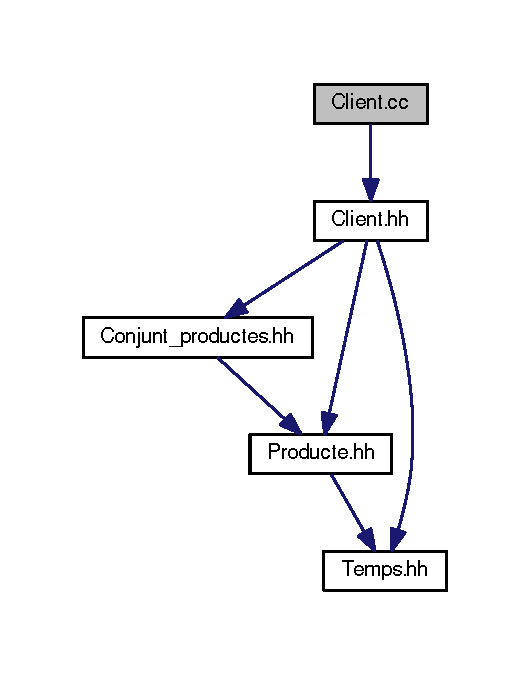
\includegraphics[width=254pt]{_client_8cc__incl}
\end{center}
\end{figure}
\subsection*{Funcions}
\begin{DoxyCompactItemize}
\item 
int \hyperlink{_client_8cc_a242d0f8a1d76d9990a9757ea9d5045a5}{calcula\-\_\-cami} (const vector$<$ \hyperlink{structseccio}{seccio} $>$ \&productes, int i, const int columnes)
\item 
void \hyperlink{_client_8cc_a863e18eda8214bd7b937afca28203350}{canvi} (vector$<$ \hyperlink{structseccio}{seccio} $>$ \&v, int a, int b)
\item 
bool \hyperlink{_client_8cc_a0ee569d71274691654f93b828db05bc4}{ordre\-\_\-lexicografic} (const vector$<$ \hyperlink{structseccio}{seccio} $>$ \&a, const vector$<$ \hyperlink{structseccio}{seccio} $>$ \&b)
\item 
void \hyperlink{_client_8cc_a46dcbde0b35706040fdc7644269132be}{consultar\-\_\-millor\-\_\-cami\-\_\-aux} (vector$<$ \hyperlink{structseccio}{seccio} $>$ \&productes, int i, vector$<$ \hyperlink{structseccio}{seccio} $>$ \&vector\-\_\-aux, int \&min, const int columnes, int actual)
\item 
pair$<$ int, int $>$ \hyperlink{_client_8cc_aa1c79131574379b4cd989a7ef172990d}{cas\-\_\-extrem} (const vector$<$ \hyperlink{structseccio}{seccio} $>$ \&productes, const int columnes)
\end{DoxyCompactItemize}


\subsection{Documentació de les Funcions}
\hypertarget{_client_8cc_a242d0f8a1d76d9990a9757ea9d5045a5}{\index{Client.\-cc@{Client.\-cc}!calcula\-\_\-cami@{calcula\-\_\-cami}}
\index{calcula\-\_\-cami@{calcula\-\_\-cami}!Client.cc@{Client.\-cc}}
\subsubsection[{calcula\-\_\-cami}]{\setlength{\rightskip}{0pt plus 5cm}int calcula\-\_\-cami (
\begin{DoxyParamCaption}
\item[{const vector$<$ {\bf seccio} $>$ \&}]{productes, }
\item[{int}]{i, }
\item[{const int}]{columnes}
\end{DoxyParamCaption}
)}}\label{_client_8cc_a242d0f8a1d76d9990a9757ea9d5045a5}


Definició a la línia 128 del fitxer Client.\-cc.


\begin{DoxyCode}
128                                                                             \{
129     \textcolor{keywordtype}{int} res = 0;
130     \textcolor{keywordflow}{if} (i == 0) res += (abs(productes[i].x - \textcolor{charliteral}{'A'}) + abs(productes[i].y - 1));
131     \textcolor{keywordflow}{else} \textcolor{keywordflow}{if} (i == productes.size()) res += (abs(productes[i-1].x - \textcolor{charliteral}{'A'}) + abs(productes[i-1].y - columnes))
      ;
132     \textcolor{keywordflow}{else} res += (abs(productes[i-1].x - productes[i].x) + abs(productes[i-1].y - productes[i].y));
133     \textcolor{keywordflow}{return} res;
134 \}
\end{DoxyCode}
\hypertarget{_client_8cc_a863e18eda8214bd7b937afca28203350}{\index{Client.\-cc@{Client.\-cc}!canvi@{canvi}}
\index{canvi@{canvi}!Client.cc@{Client.\-cc}}
\subsubsection[{canvi}]{\setlength{\rightskip}{0pt plus 5cm}void canvi (
\begin{DoxyParamCaption}
\item[{vector$<$ {\bf seccio} $>$ \&}]{v, }
\item[{int}]{a, }
\item[{int}]{b}
\end{DoxyParamCaption}
)}}\label{_client_8cc_a863e18eda8214bd7b937afca28203350}


Definició a la línia 136 del fitxer Client.\-cc.


\begin{DoxyCode}
136                                             \{
137     \hyperlink{structseccio}{seccio} aux;
138     aux = v[a];
139     v[a] = v[b];
140     v[b] = aux;
141 \}
\end{DoxyCode}
\hypertarget{_client_8cc_a0ee569d71274691654f93b828db05bc4}{\index{Client.\-cc@{Client.\-cc}!ordre\-\_\-lexicografic@{ordre\-\_\-lexicografic}}
\index{ordre\-\_\-lexicografic@{ordre\-\_\-lexicografic}!Client.cc@{Client.\-cc}}
\subsubsection[{ordre\-\_\-lexicografic}]{\setlength{\rightskip}{0pt plus 5cm}bool ordre\-\_\-lexicografic (
\begin{DoxyParamCaption}
\item[{const vector$<$ {\bf seccio} $>$ \&}]{a, }
\item[{const vector$<$ {\bf seccio} $>$ \&}]{b}
\end{DoxyParamCaption}
)}}\label{_client_8cc_a0ee569d71274691654f93b828db05bc4}


Definició a la línia 144 del fitxer Client.\-cc.


\begin{DoxyCode}
144                                                                           \{
145     \textcolor{keywordtype}{int} i = 0;
146     \textcolor{keywordflow}{while} (i != a.size()) \{
147         \textcolor{keywordflow}{if} (a[i].x < b[i].x) \textcolor{keywordflow}{return} \textcolor{keyword}{true};
148         \textcolor{keywordflow}{else} \textcolor{keywordflow}{if} (a[i].x > b[i].x) \textcolor{keywordflow}{return} \textcolor{keyword}{false};
149   \textcolor{keywordflow}{else} \textcolor{keywordflow}{if} (a[i].y < b[i].y) \textcolor{keywordflow}{return} \textcolor{keyword}{true};
150   \textcolor{keywordflow}{else} \textcolor{keywordflow}{if} (a[i].y > b[i].y) \textcolor{keywordflow}{return} \textcolor{keyword}{false};
151         \textcolor{keywordflow}{else} i++;
152     \}
153     \textcolor{comment}{//Cas que siguin iguals (que mai es donara)}
154     \textcolor{keywordflow}{return} \textcolor{keyword}{true};
155 \}
\end{DoxyCode}
\hypertarget{_client_8cc_a46dcbde0b35706040fdc7644269132be}{\index{Client.\-cc@{Client.\-cc}!consultar\-\_\-millor\-\_\-cami\-\_\-aux@{consultar\-\_\-millor\-\_\-cami\-\_\-aux}}
\index{consultar\-\_\-millor\-\_\-cami\-\_\-aux@{consultar\-\_\-millor\-\_\-cami\-\_\-aux}!Client.cc@{Client.\-cc}}
\subsubsection[{consultar\-\_\-millor\-\_\-cami\-\_\-aux}]{\setlength{\rightskip}{0pt plus 5cm}void consultar\-\_\-millor\-\_\-cami\-\_\-aux (
\begin{DoxyParamCaption}
\item[{vector$<$ {\bf seccio} $>$ \&}]{productes, }
\item[{int}]{i, }
\item[{vector$<$ {\bf seccio} $>$ \&}]{vector\-\_\-aux, }
\item[{int \&}]{min, }
\item[{const int}]{columnes, }
\item[{int}]{actual}
\end{DoxyParamCaption}
)}}\label{_client_8cc_a46dcbde0b35706040fdc7644269132be}


Definició a la línia 157 del fitxer Client.\-cc.


\begin{DoxyCode}
157                                                                                                            
                                  \{
158     \textcolor{keywordflow}{if} (i != productes.size()) \{
159         \textcolor{keywordflow}{for} (\textcolor{keywordtype}{int} j = i; j < productes.size(); j++) \{
160             \hyperlink{_client_8cc_a863e18eda8214bd7b937afca28203350}{canvi}(productes, i, j);
161             \textcolor{keywordtype}{int} aux = \hyperlink{_client_8cc_a242d0f8a1d76d9990a9757ea9d5045a5}{calcula\_cami}(productes,i,columnes);
162             actual += aux;
163             \textcolor{keywordflow}{if} (min >=actual) \hyperlink{_client_8cc_a46dcbde0b35706040fdc7644269132be}{consultar\_millor\_cami\_aux}(productes, i+1, vector\_aux
      , min, columnes, actual);
164             actual -= aux;
165             \hyperlink{_client_8cc_a863e18eda8214bd7b937afca28203350}{canvi}(productes,i,j);
166         \}
167     \}
168     \textcolor{keywordflow}{else} \{
169         \textcolor{keywordtype}{int} aux = \hyperlink{_client_8cc_a242d0f8a1d76d9990a9757ea9d5045a5}{calcula\_cami}(productes,productes.size(),columnes);
170         actual += aux;
171         \textcolor{keywordflow}{if} (min > actual) \{
172             min = actual;
173             \textcolor{keywordflow}{for} (\textcolor{keywordtype}{int} i = 0; i < productes.size(); i++) vector\_aux[i] = productes[i];
174         \}
175         \textcolor{keywordflow}{else} \textcolor{keywordflow}{if} (min == actual) \{
176             \textcolor{keywordflow}{if} (\hyperlink{_client_8cc_a0ee569d71274691654f93b828db05bc4}{ordre\_lexicografic}(productes, vector\_aux)) \{
177                 \textcolor{keywordflow}{for} (\textcolor{keywordtype}{int} i = 0; i < productes.size(); i++) vector\_aux[i] = productes[i];
178             \}
179         \}
180         actual -= aux;
181     \}
182 \}
\end{DoxyCode}
\hypertarget{_client_8cc_aa1c79131574379b4cd989a7ef172990d}{\index{Client.\-cc@{Client.\-cc}!cas\-\_\-extrem@{cas\-\_\-extrem}}
\index{cas\-\_\-extrem@{cas\-\_\-extrem}!Client.cc@{Client.\-cc}}
\subsubsection[{cas\-\_\-extrem}]{\setlength{\rightskip}{0pt plus 5cm}pair$<$int,int$>$ cas\-\_\-extrem (
\begin{DoxyParamCaption}
\item[{const vector$<$ {\bf seccio} $>$ \&}]{productes, }
\item[{const int}]{columnes}
\end{DoxyParamCaption}
)}}\label{_client_8cc_aa1c79131574379b4cd989a7ef172990d}


Definició a la línia 185 del fitxer Client.\-cc.


\begin{DoxyCode}
185                                                                              \{
186     \textcolor{comment}{//Funció auxiliar per mirar si tenim productes a A1 o Acolumnes}
187     \textcolor{keywordtype}{int} j = 0;
188     \textcolor{keywordtype}{int} i = productes.size();
189     \textcolor{keywordflow}{if} (productes[0].x == \textcolor{charliteral}{'A'} and productes[0].y == 1) j++;
190     \textcolor{keywordflow}{if} (productes[i-1].x == \textcolor{charliteral}{'A'} and productes[i-1].y == columnes) i--;
191     \textcolor{keywordflow}{return} make\_pair(j,i);
192 \}
\end{DoxyCode}

\hypertarget{_client_8hh}{\section{Referència del Fitxer Client.\-hh}
\label{_client_8hh}\index{Client.\-hh@{Client.\-hh}}
}


Classe \hyperlink{class_client}{Client}.  


Inclou el graf de dependències per a Client.\-hh\-:\nopagebreak
\begin{figure}[H]
\begin{center}
\leavevmode
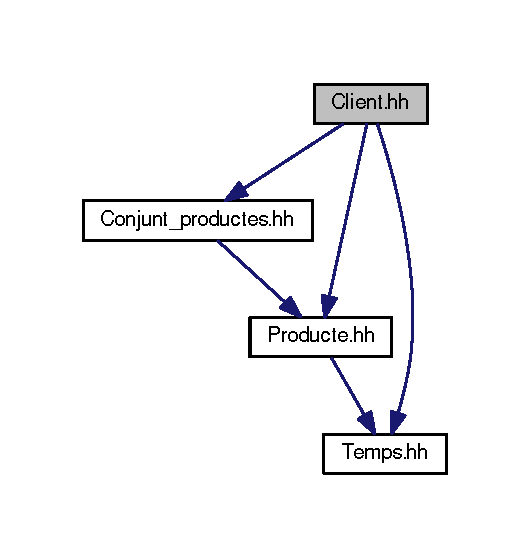
\includegraphics[width=254pt]{_client_8hh__incl}
\end{center}
\end{figure}
\subsection*{Classes}
\begin{DoxyCompactItemize}
\item 
struct \hyperlink{structseccio}{seccio}
\item 
class \hyperlink{class_client}{Client}
\begin{DoxyCompactList}\small\item\em Respresenta un \hyperlink{class_client}{Client} com a contenidor de Seccions i \hyperlink{class_temps}{Temps}. \end{DoxyCompactList}\end{DoxyCompactItemize}


\subsection{Descripció Detallada}
Classe \hyperlink{class_client}{Client}. 

Definició al fitxer \hyperlink{_client_8hh_source}{Client.\-hh}.


\hypertarget{_conjunt__clients_8cc}{\section{Referència del Fitxer Conjunt\-\_\-clients.\-cc}
\label{_conjunt__clients_8cc}\index{Conjunt\-\_\-clients.\-cc@{Conjunt\-\_\-clients.\-cc}}
}
Inclou el graf de dependències per a Conjunt\-\_\-clients.\-cc\-:\nopagebreak
\begin{figure}[H]
\begin{center}
\leavevmode
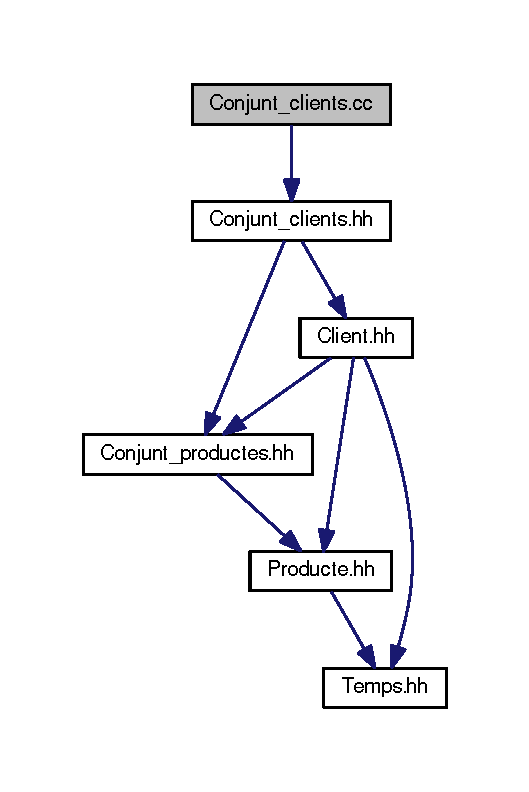
\includegraphics[width=254pt]{_conjunt__clients_8cc__incl}
\end{center}
\end{figure}

\hypertarget{_conjunt__clients_8hh}{\section{Referència del Fitxer Conjunt\-\_\-clients.\-hh}
\label{_conjunt__clients_8hh}\index{Conjunt\-\_\-clients.\-hh@{Conjunt\-\_\-clients.\-hh}}
}


Classe \hyperlink{class_conjunt__clients}{Conjunt\-\_\-clients}.  


Inclou el graf de dependències per a Conjunt\-\_\-clients.\-hh\-:\nopagebreak
\begin{figure}[H]
\begin{center}
\leavevmode
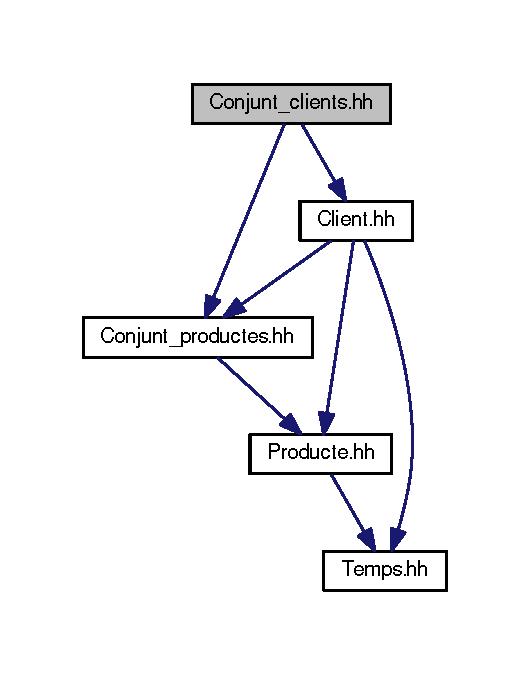
\includegraphics[width=254pt]{_conjunt__clients_8hh__incl}
\end{center}
\end{figure}
\subsection*{Classes}
\begin{DoxyCompactItemize}
\item 
class \hyperlink{class_conjunt__clients}{Conjunt\-\_\-clients}
\begin{DoxyCompactList}\small\item\em Respresenta un Conjunt de clients com a contenidor de Clients. \end{DoxyCompactList}\end{DoxyCompactItemize}


\subsection{Descripció Detallada}
Classe \hyperlink{class_conjunt__clients}{Conjunt\-\_\-clients}. 

Definició al fitxer \hyperlink{_conjunt__clients_8hh_source}{Conjunt\-\_\-clients.\-hh}.


\hypertarget{_conjunt__productes_8cc}{\section{Referència del Fitxer Conjunt\-\_\-productes.\-cc}
\label{_conjunt__productes_8cc}\index{Conjunt\-\_\-productes.\-cc@{Conjunt\-\_\-productes.\-cc}}
}
Inclou el graf de dependències per a Conjunt\-\_\-productes.\-cc\-:\nopagebreak
\begin{figure}[H]
\begin{center}
\leavevmode
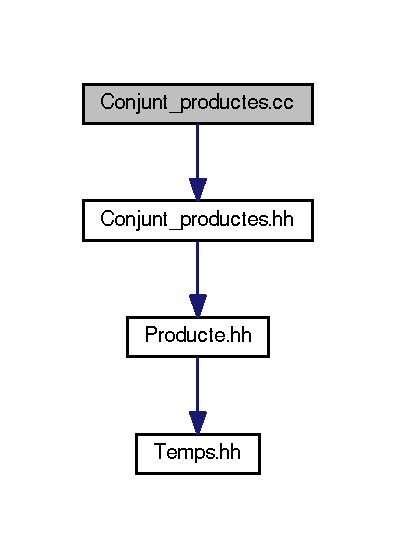
\includegraphics[width=190pt]{_conjunt__productes_8cc__incl}
\end{center}
\end{figure}

\hypertarget{_conjunt__productes_8hh}{\section{Referència del Fitxer Conjunt\-\_\-productes.\-hh}
\label{_conjunt__productes_8hh}\index{Conjunt\-\_\-productes.\-hh@{Conjunt\-\_\-productes.\-hh}}
}


Classe \hyperlink{class_conjunt__productes}{Conjunt\-\_\-productes}.  


Inclou el graf de dependències per a Conjunt\-\_\-productes.\-hh\-:\nopagebreak
\begin{figure}[H]
\begin{center}
\leavevmode
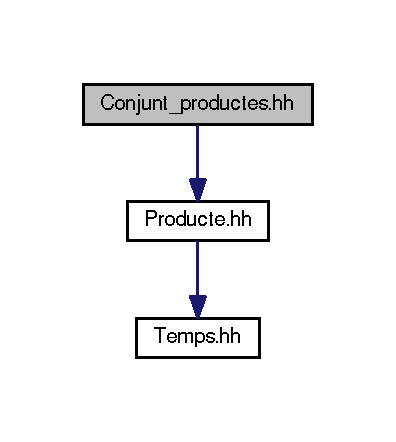
\includegraphics[width=190pt]{_conjunt__productes_8hh__incl}
\end{center}
\end{figure}
\subsection*{Classes}
\begin{DoxyCompactItemize}
\item 
class \hyperlink{class_conjunt__productes}{Conjunt\-\_\-productes}
\begin{DoxyCompactList}\small\item\em Respresenta un Conjunt de productes con a contenidor de Productes. \end{DoxyCompactList}\end{DoxyCompactItemize}


\subsection{Descripció Detallada}
Classe \hyperlink{class_conjunt__productes}{Conjunt\-\_\-productes}. 

Definició al fitxer \hyperlink{_conjunt__productes_8hh_source}{Conjunt\-\_\-productes.\-hh}.


\hypertarget{_producte_8cc}{\section{Referència del Fitxer Producte.\-cc}
\label{_producte_8cc}\index{Producte.\-cc@{Producte.\-cc}}
}
Inclou el graf de dependències per a Producte.\-cc\-:\nopagebreak
\begin{figure}[H]
\begin{center}
\leavevmode
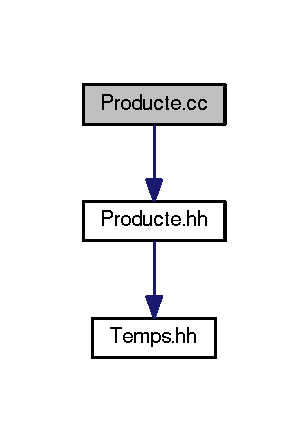
\includegraphics[width=148pt]{_producte_8cc__incl}
\end{center}
\end{figure}

\hypertarget{_producte_8hh}{\section{Referència del Fitxer Producte.\-hh}
\label{_producte_8hh}\index{Producte.\-hh@{Producte.\-hh}}
}


Classe \hyperlink{class_producte}{Producte}.  


Inclou el graf de dependències per a Producte.\-hh\-:\nopagebreak
\begin{figure}[H]
\begin{center}
\leavevmode
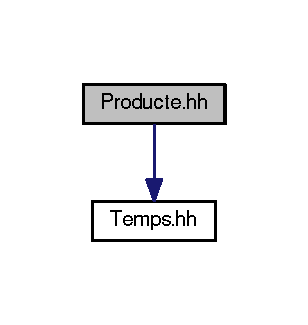
\includegraphics[width=148pt]{_producte_8hh__incl}
\end{center}
\end{figure}
\subsection*{Classes}
\begin{DoxyCompactItemize}
\item 
class \hyperlink{class_producte}{Producte}
\begin{DoxyCompactList}\small\item\em Respresenta un \hyperlink{class_producte}{Producte} com a contenidor d'un id, la seva posició a la graella, un temps de cobrament i un preu. \end{DoxyCompactList}\end{DoxyCompactItemize}


\subsection{Descripció Detallada}
Classe \hyperlink{class_producte}{Producte}. 

Definició al fitxer \hyperlink{_producte_8hh_source}{Producte.\-hh}.


\hypertarget{program_8cc}{\section{Referència del Fitxer program.\-cc}
\label{program_8cc}\index{program.\-cc@{program.\-cc}}
}
Inclou el graf de dependències per a program.\-cc\-:\nopagebreak
\begin{figure}[H]
\begin{center}
\leavevmode
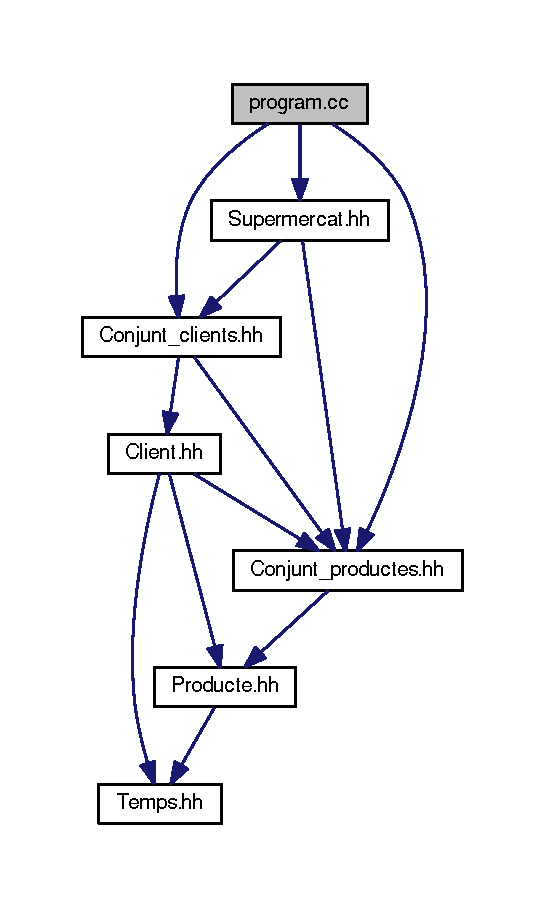
\includegraphics[width=262pt]{program_8cc__incl}
\end{center}
\end{figure}
\subsection*{Funcions}
\begin{DoxyCompactItemize}
\item 
int \hyperlink{program_8cc_ae66f6b31b5ad750f1fe042a706a4e3d4}{main} ()
\end{DoxyCompactItemize}


\subsection{Documentació de les Funcions}
\hypertarget{program_8cc_ae66f6b31b5ad750f1fe042a706a4e3d4}{\index{program.\-cc@{program.\-cc}!main@{main}}
\index{main@{main}!program.cc@{program.\-cc}}
\subsubsection[{main}]{\setlength{\rightskip}{0pt plus 5cm}int main (
\begin{DoxyParamCaption}
{}
\end{DoxyParamCaption}
)}}\label{program_8cc_ae66f6b31b5ad750f1fe042a706a4e3d4}


Definició a la línia 5 del fitxer program.\-cc.


\begin{DoxyCode}
5            \{
6     \textcolor{keywordtype}{string} p;
7     \hyperlink{class_supermercat}{Supermercat} s;
8     \hyperlink{class_conjunt__productes}{Conjunt\_productes} cp;
9     \hyperlink{class_conjunt__productes}{Conjunt\_productes} cp\_aux;   \textcolor{comment}{//sempre buit}
10     \hyperlink{class_conjunt__clients}{Conjunt\_clients} cc;
11     \hyperlink{class_conjunt__clients}{Conjunt\_clients} cc\_aux;     \textcolor{comment}{//sempre buit}
12     \textcolor{keywordtype}{int} col,rengles, caixes, n;
13     cin >> p;
14     \textcolor{keywordtype}{bool} ini\_supermercat, ini\_clients;
15     ini\_supermercat = ini\_clients = \textcolor{keyword}{false};
16     \textcolor{keywordflow}{while} (p != \textcolor{stringliteral}{"sortir"}) \{
17         \textcolor{keywordflow}{if} (p == \textcolor{stringliteral}{"inicialitzar"}) \{
18             ini\_supermercat = \textcolor{keyword}{true};
19             ini\_clients = \textcolor{keyword}{false};
20             cin >> rengles >> col >> caixes >> n;
21             s.\hyperlink{class_supermercat_ad983ec7f34920bbbd56225b6c21af2b3}{afegir\_parametres\_supermercat}(rengles,col,caixes,n);
22             cp = cp\_aux;
23             s.\hyperlink{class_supermercat_abe76363df7d0d1a759a4539d70187204}{afegir\_n\_productes}(n,cp);  
24         \}
25         \textcolor{keywordflow}{else} \textcolor{keywordflow}{if} (p == \textcolor{stringliteral}{"carregar"}) \{
26             \textcolor{keywordtype}{int} n\_clients;
27             cin >> n\_clients;
28             cc = cc\_aux;
29             \textcolor{keywordflow}{if} (ini\_supermercat)
30             \{
31                 ini\_clients = \textcolor{keyword}{true};
32                 cc.\hyperlink{class_conjunt__clients_adb51222eb8d58efbf90a6229409d88d2}{afegir\_n\_clients}(n\_clients, cp);
33             \}
34             \textcolor{keywordflow}{else}
35                 cout << \textcolor{stringliteral}{"error"} << endl;
36         \}
37         \textcolor{keywordflow}{else} \textcolor{keywordflow}{if} (p == \textcolor{stringliteral}{"informacio"}) \{
38             \textcolor{keywordtype}{string} id;
39             cin >> id;
40             cout << \textcolor{stringliteral}{"informacio "} << \textcolor{keywordtype}{id} << \textcolor{stringliteral}{":"} << endl;
41             \textcolor{keywordflow}{if} (ini\_supermercat)
42                 cp.\hyperlink{class_conjunt__productes_a881cfe5494d2fac0354fdc82636fc5ff}{informacio\_producte}(\textcolor{keywordtype}{id});
43             \textcolor{keywordflow}{else}
44                 cout << \textcolor{stringliteral}{"error"} << endl << endl;
45         \}
46         \textcolor{keywordflow}{else} \textcolor{keywordflow}{if} (p == \textcolor{stringliteral}{"productes"}) \{
47             \textcolor{keywordtype}{string} \hyperlink{structseccio}{seccio};
48             cin >> seccio;
49             cout << \textcolor{stringliteral}{"productes "} << seccio << \textcolor{stringliteral}{":"} << endl;
50             \textcolor{keywordflow}{if} (ini\_supermercat)
51             \{
52                 \textcolor{keywordflow}{if} ((seccio[0] - \textcolor{charliteral}{'A'} > rengles) or (col - \textcolor{keywordtype}{int}(seccio[1]-\textcolor{charliteral}{'0'}) < 0)) \{
53                     cout << \textcolor{stringliteral}{"error"} << endl << endl;
54                 \}
55                 \textcolor{keywordflow}{else}
56                     s.\hyperlink{class_supermercat_add121e2ed13fa94e85accf3dc60cfa44}{productes\_seccio}(seccio);
57             \}
58             \textcolor{keywordflow}{else}
59                 cout << \textcolor{stringliteral}{"error"} << endl << endl;
60         \}
61         \textcolor{keywordflow}{else} \textcolor{keywordflow}{if} (p == \textcolor{stringliteral}{"millor"}) \{
62             cin >> p;
63             \textcolor{keywordflow}{if} (p == \textcolor{stringliteral}{"cami"}) \{
64                 \textcolor{keywordtype}{int} comprador\_id;
65                 cin >> comprador\_id;
66                 cout << \textcolor{stringliteral}{"millor cami "} << comprador\_id << \textcolor{stringliteral}{":"} << endl;
67                 \textcolor{keywordflow}{if} (ini\_supermercat and ini\_clients)
68                     cc.\hyperlink{class_conjunt__clients_a1ee4708cf975dc683f15f7cfb60cb146}{consultar\_millor\_cami\_client}(comprador\_id,col);
69                 \textcolor{keywordflow}{else}
70                 \{
71                     \textcolor{comment}{//cout << "Supermercat: " << ini\_supermercat << " - Clients: " << ini\_clients << endl;}
72                     cout << \textcolor{stringliteral}{"error"} << endl << endl;
73                 \}
74             \}
75             \textcolor{keywordflow}{else} cout << \textcolor{stringliteral}{"error"} << endl << endl;
76         \}
77         \textcolor{keywordflow}{else} \textcolor{keywordflow}{if} (p == \textcolor{stringliteral}{"simular"}) \{
78             cin >> p;
79             \textcolor{keywordflow}{if} (p == \textcolor{stringliteral}{"pagament"}) \{
80                 cout << \textcolor{stringliteral}{"simular pagament:"} << endl;
81                 \textcolor{keywordflow}{if}(ini\_supermercat and ini\_clients)
82                 \{
83                     \textcolor{keywordtype}{int} n\_simulacions;
84                     cin >> n\_simulacions;
85                     s.\hyperlink{class_supermercat_aac66c4aa58a3d095f4baa10a3ea05f1b}{simulacio}(n\_simulacions,cc);
86                     
87                 \}
88                 \textcolor{keywordflow}{else}
89                     cout << \textcolor{stringliteral}{"error"} << endl << endl;
90             \}
91             \textcolor{keywordflow}{else} cout << \textcolor{stringliteral}{"error"} << endl << endl;
92         \}
93         
94         \textcolor{keywordflow}{else} cout << \textcolor{stringliteral}{"error"} << endl << endl;
95         cin >> p;
96   \}
97 
98 \}
\end{DoxyCode}

\hypertarget{_supermercat_8cc}{\section{Referència del Fitxer Supermercat.\-cc}
\label{_supermercat_8cc}\index{Supermercat.\-cc@{Supermercat.\-cc}}
}
Inclou el graf de dependències per a Supermercat.\-cc\-:\nopagebreak
\begin{figure}[H]
\begin{center}
\leavevmode
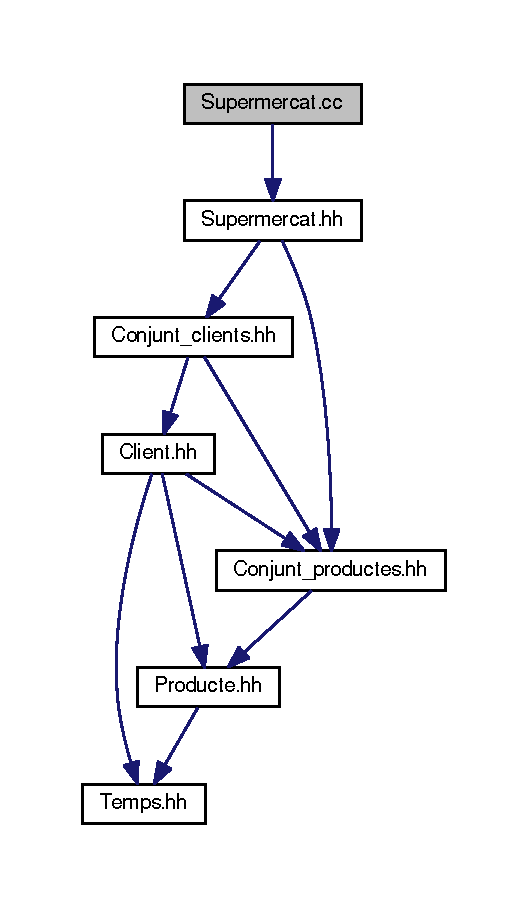
\includegraphics[width=254pt]{_supermercat_8cc__incl}
\end{center}
\end{figure}
\subsection*{Funcions}
\begin{DoxyCompactItemize}
\item 
void \hyperlink{_supermercat_8cc_a40c9e72e542bee4460d1a786adfb6eeb}{afegir\-\_\-producte\-\_\-supermercat} (string producte\-\_\-id, string \hyperlink{structseccio}{seccio}, vector$<$ vector$<$ set$<$ string $>$ $>$ $>$ \&seccions)
\item 
\hyperlink{class_temps}{Temps} \hyperlink{_supermercat_8cc_a8cd29707c0a2d6f7207858b0f98573e4}{temps\-\_\-espera\-\_\-aux} (\hyperlink{class_temps}{Temps} t1, \hyperlink{class_temps}{Temps} t2)
\end{DoxyCompactItemize}


\subsection{Documentació de les Funcions}
\hypertarget{_supermercat_8cc_a40c9e72e542bee4460d1a786adfb6eeb}{\index{Supermercat.\-cc@{Supermercat.\-cc}!afegir\-\_\-producte\-\_\-supermercat@{afegir\-\_\-producte\-\_\-supermercat}}
\index{afegir\-\_\-producte\-\_\-supermercat@{afegir\-\_\-producte\-\_\-supermercat}!Supermercat.cc@{Supermercat.\-cc}}
\subsubsection[{afegir\-\_\-producte\-\_\-supermercat}]{\setlength{\rightskip}{0pt plus 5cm}void afegir\-\_\-producte\-\_\-supermercat (
\begin{DoxyParamCaption}
\item[{string}]{producte\-\_\-id, }
\item[{string}]{seccio, }
\item[{vector$<$ vector$<$ set$<$ string $>$ $>$ $>$ \&}]{seccions}
\end{DoxyParamCaption}
)}}\label{_supermercat_8cc_a40c9e72e542bee4460d1a786adfb6eeb}


Definició a la línia 59 del fitxer Supermercat.\-cc.


\begin{DoxyCode}
60 \{
61     \textcolor{keywordtype}{int} x, y;
62     x = \hyperlink{structseccio}{seccio}[0] - \textcolor{charliteral}{'A'};
63     y = \hyperlink{structseccio}{seccio}[1] - \textcolor{charliteral}{'0'} - 1;
64     seccions[x][y].insert(producte\_id);
65 \}
\end{DoxyCode}
\hypertarget{_supermercat_8cc_a8cd29707c0a2d6f7207858b0f98573e4}{\index{Supermercat.\-cc@{Supermercat.\-cc}!temps\-\_\-espera\-\_\-aux@{temps\-\_\-espera\-\_\-aux}}
\index{temps\-\_\-espera\-\_\-aux@{temps\-\_\-espera\-\_\-aux}!Supermercat.cc@{Supermercat.\-cc}}
\subsubsection[{temps\-\_\-espera\-\_\-aux}]{\setlength{\rightskip}{0pt plus 5cm}{\bf Temps} temps\-\_\-espera\-\_\-aux (
\begin{DoxyParamCaption}
\item[{{\bf Temps}}]{t1, }
\item[{{\bf Temps}}]{t2}
\end{DoxyParamCaption}
)}}\label{_supermercat_8cc_a8cd29707c0a2d6f7207858b0f98573e4}


Definició a la línia 97 del fitxer Supermercat.\-cc.


\begin{DoxyCode}
98 \{                                           \textcolor{comment}{//t2: instant de pagar del següent client}
99     \hyperlink{class_temps}{Temps} t\_out(0,0,0);
100     \textcolor{keywordflow}{if} (t1.\hyperlink{class_temps_ad7dfb62dadfa4f00adf58936d9cba7ed}{compara\_temps}(t2) <= 0)
101     \{
102         \textcolor{keywordtype}{double} t1\_aux = t1.\hyperlink{class_temps_a766b7d3c06cd8320b13854d31bac4251}{consultar\_segons}();
103         t1\_aux += (t1.\hyperlink{class_temps_a8af21ff997b0893f9a2f2f8eccf8dc8c}{consultar\_minuts}())*60;
104         t1\_aux += (t1.\hyperlink{class_temps_ae9f07c4548a30807e3056f217e837eb3}{consultar\_hores}())*3600;
105         
106         \textcolor{keywordtype}{double} t2\_aux = t2.\hyperlink{class_temps_a766b7d3c06cd8320b13854d31bac4251}{consultar\_segons}();
107         t2\_aux += (t2.\hyperlink{class_temps_a8af21ff997b0893f9a2f2f8eccf8dc8c}{consultar\_minuts}())*60;
108         t2\_aux += (t2.\hyperlink{class_temps_ae9f07c4548a30807e3056f217e837eb3}{consultar\_hores}())*3600;
109         
110         \textcolor{keywordtype}{double} out = t2\_aux - t1\_aux;
111         t\_out.modificar\_segons(out);
112         t\_out.actualitza\_temps();
113     \}
114     
115     \textcolor{keywordflow}{return} t\_out;
116 \}
\end{DoxyCode}

\hypertarget{_supermercat_8hh}{\section{Referència del Fitxer Supermercat.\-hh}
\label{_supermercat_8hh}\index{Supermercat.\-hh@{Supermercat.\-hh}}
}


Classe \hyperlink{class_supermercat}{Supermercat}.  


Inclou el graf de dependències per a Supermercat.\-hh\-:\nopagebreak
\begin{figure}[H]
\begin{center}
\leavevmode
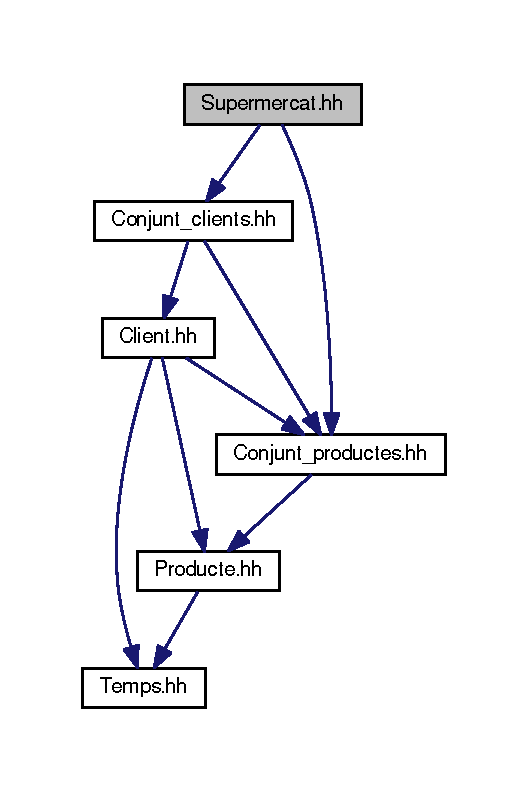
\includegraphics[width=254pt]{_supermercat_8hh__incl}
\end{center}
\end{figure}
\subsection*{Classes}
\begin{DoxyCompactItemize}
\item 
struct \hyperlink{struct_caixa}{Caixa}
\item 
class \hyperlink{class_supermercat}{Supermercat}
\begin{DoxyCompactList}\small\item\em Respresenta un \hyperlink{class_supermercat}{Supermercat} com a contenidor de Matriu de sets i un vector de Caixes. \end{DoxyCompactList}\end{DoxyCompactItemize}


\subsection{Descripció Detallada}
Classe \hyperlink{class_supermercat}{Supermercat}. 

Definició al fitxer \hyperlink{_supermercat_8hh_source}{Supermercat.\-hh}.


\hypertarget{_temps_8cc}{\section{Referència del Fitxer Temps.\-cc}
\label{_temps_8cc}\index{Temps.\-cc@{Temps.\-cc}}
}
Inclou el graf de dependències per a Temps.\-cc\-:\nopagebreak
\begin{figure}[H]
\begin{center}
\leavevmode
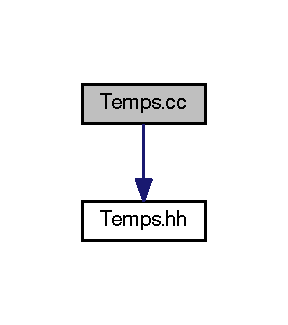
\includegraphics[width=138pt]{_temps_8cc__incl}
\end{center}
\end{figure}

\hypertarget{_temps_8hh}{\section{Referència del Fitxer Temps.\-hh}
\label{_temps_8hh}\index{Temps.\-hh@{Temps.\-hh}}
}


Classe \hyperlink{class_temps}{Temps}.  


\subsection*{Classes}
\begin{DoxyCompactItemize}
\item 
class \hyperlink{class_temps}{Temps}
\begin{DoxyCompactList}\small\item\em Respresentacio del temps en hores,minuts i segons. \end{DoxyCompactList}\end{DoxyCompactItemize}


\subsection{Descripció Detallada}
Classe \hyperlink{class_temps}{Temps}. 

Definició al fitxer \hyperlink{_temps_8hh_source}{Temps.\-hh}.


%--- End generated contents ---

% Index
\newpage
\phantomsection
\addcontentsline{toc}{chapter}{Índex}
\printindex

\end{document}
